\documentclass[11pt]{article}
\usepackage{graphics,graphicx}
%\usepackage[dvips]{graphics,graphicx}
\DeclareGraphicsExtensions{.ps,.jpg,.eps,.pdf,.png}
\usepackage{boxedminipage,amsmath,amsfonts}
\usepackage{url}
%\usepackage{secdot}
%\usepackage{natbib}
\usepackage{verbatim}
%\usepackage{moreverb}
\usepackage{enumerate}
\usepackage{makeidx}
\usepackage{own}
\bibliographystyle{plain}
\makeindex

%%%%%
% some other macros
\newcommand{\figurepath}{./figures}
\newcommand{\bibpath}{/Users/kmartin/Documents/files/misc}
\newcommand{\figfiletype}{pdf}

%Brad Bell Macros

% Latex macros defined for all the CppAD documentation:
\newcommand{\T}{ {\rm T} }
\newcommand{\R}{ {\bf R} }
\newcommand{\C}{ {\bf C} }
\newcommand{\D}[2]{ \frac{\partial #1}{\partial #2} }
\newcommand{\DD}[3]{ \frac{\partial^2 #1}{\partial #2 \partial #3} }
\newcommand{\Dpow}[2]{ \frac{\partial^{#1}}{\partial  {#2}^{#1}} }
\newcommand{\dpow}[2]{ \frac{ {\rm d}^{#1}}{{\rm d}\, {#2}^{#1}} }

% Define the hangref environment used for the References list:
\newenvironment{hangref}
  {\begin{list}{}{\setlength{\itemsep}{4pt}
  \setlength{\parsep}{0pt}\setlength{\leftmargin}{+\parindent}
  \setlength{\itemindent}{-\parindent}}}{\end{list}}

% Set the page margins to 1 inch all around:
\marginparwidth 0pt\marginparsep 0pt \topskip 0pt\headsep
0pt\headheight 0pt \oddsidemargin 0pt\evensidemargin 0pt
\textwidth 6.5in \topmargin 0pt\textheight 9.0in
\newtheorem{theorem}{Theorem}

   
%%%%Added by Leo%%%%
\newcounter{Fig}
\renewcommand{\theFig}{\arabic{Fig}}
\newcommand{\Fig}[2]{\refstepcounter{Fig} \label{#1}
                     {\small\bf Figure \theFig.} {\small\sl #2 \par}}

\setcounter{topnumber}{3}
\renewcommand{\topfraction}{.9}
\setcounter{bottomnumber}{3}
\renewcommand{\bottomfraction}{.9}
\setcounter{totalnumber}{4}
\renewcommand{\textfraction}{.1}
\setlength{\floatsep}{.25in}
\setlength{\intextsep}{.25in}

\setlength{\fboxrule}{2\fboxrule} \setlength{\fboxsep}{3\fboxsep}

\newcommand{\Sa}{8pt}
\newcommand{\Sb}{0pt}

\renewcommand{\_}{{\char"5F}}
\renewcommand{\{}{{\char"7B}}
\renewcommand{\}}{{\char"7D}}
\renewcommand{\^}{{\char"0D}}

\let\accute= \'
\renewcommand{\'}{{\char"0D}}

\newcommand{\bfit}{\bfseries\itshape}

\newlength{\extopskip} \newlength{\exbottomskip}
\setlength{\exbottomskip}{1\baselineskip}
\addtolength{\exbottomskip}{-5.0pt}
\setlength{\extopskip}{1\exbottomskip}
\addtolength{\extopskip}{-1\parskip}

\newenvironment{Example}{\vspace{1\extopskip}\noindent\hspace*{2em}
                         \frenchspacing\small
                         \tt\begin{tabular}{@{}l@{}}}{
                         \end{tabular}\\[1\exbottomskip]}

\newcommand{\Titem}{\item[$\triangleright$]}
\newcommand{\Ditem}{\item[$\diamond$]}

\newenvironment{Itemize}{\begin{quote}\normalsize
   \baselineskip 20pt plus .3pt minus .1pt \begin{itemize}}
   {\end{itemize}\end{quote}}
   % Set path to folder containing figures
\newcommand{\FigureFolder}{figures}

\newif\ifknitro \knitrofalse    % change to \knitrotrue once we get knitro connected again
\newif\ifipopt  \ipopttrue      % change to \ipopttrue  once we get the build problems sorted out


% We use a number of URLs that point to software downloads. These locations are forever changing,
% and maintaining them is a nightmare. All the URLs are gathered here, so that we can at least
% get away with making changes only once...
\newcommand{\UrlAmpl}{http://www.ampl.com}
\newcommand{\UrlAmplSandia}{http://netlib.sandia.gov/ampl/}
\newcommand{\UrlAmplSolvers}{http://netlib.sandia.gov/cgi-bin/netlib/netlibfiles.tar?filename=netlib/ampl/solvers}
\newcommand{\UrlApacheFileupload}{http://jakarta.apache.org/commons/fileupload/}
\newcommand{\UrlBlas}{ftp://www.netlib.org/blas/blas.tgz}
\newcommand{\UrlBonmin}{http://projects.coin-or.org/Bonmin}
\newcommand{\UrlBuildtools}{http://projects.coin-or.org/BuildTools}
\newcommand{\UrlCbc}{http://projects.coin-or.org/Cbc}
\newcommand{\UrlCgl}{http://projects.coin-or.org/Cgl}
\newcommand{\UrlCl}{http://www.microsoft.com/express/download/\#webInstall}
\newcommand{\UrlClp}{http://projects.coin-or.org/Clp}
\newcommand{\UrlCoinConfig}{https://projects.coin-or.org/BuildTools/wiki/user-configure\#PreparingtheCompilation}
\newcommand{\UrlCoinConfigure}{http://projects.coin-or.org/BuildTools/wiki/user-configure\#CommandLineArgumentsforconfigure}
\newcommand{\UrlCoinCygwin}{http://projects.coin-or.org/BuildTools/wiki/current-issues}
\newcommand{\UrlCoinDownload}{http://projects.coin-or.org/BuildTools/wiki/user-download\#DownloadingtheSourceCode}
\newcommand{\UrlCoinNames}{https://projects.coin-or.org/CoinBinary/wiki/ArchiveNamingConventions}
\newcommand{\UrlCoinProjects}{http://www.coin-or.org/projects/}
\newcommand{\UrlCoinUtils}{http://projects.coin-or.org/CoinUtils}
\newcommand{\UrlCouenne}{http://projects.coin-or.org/Couenne}
\newcommand{\UrlCplex}{http://www.ilog.com/products/cplex/}
\newcommand{\UrlCppad}{http://projects.coin-or.org/CppAD}
\newcommand{\UrlCygwinMake}{http://www.cmake.org/files/cygwin/make.exe}
\newcommand{\UrlCygwinSetup}{http://www.cygwin.com/setup.exe}
\newcommand{\UrlDoxygen}{http://www.doxygen.org}
\newcommand{\UrlDylp}{http://projects.coin-or.org/DyLP}
\newcommand{\UrlEpl}{http://www.eclipse.org/legal/epl-v10.html}
\newcommand{\UrlFToC}{http://www.netlib.org/f2c}
\newcommand{\UrlFToCBin}{http://www.netlib.org/f2c/mswin/}
\newcommand{\UrlFToCZip}{http://www.netlib.org/f2c/libf2c.zip}
\newcommand{\UrlGgs}{http://www.g95.org}
\newcommand{\UrlGamslinks}{https://projects.coin-or.org/svn/GAMSlinks/trunk}
\newcommand{\UrlGcc}{http://gcc.gnu.org}
\newcommand{\UrlGfortran}{http://gcc.gnu.org/fortran/}
\newcommand{\UrlGlpk}{http://www.gnu.org/software/glpk/}
\newcommand{\UrlGlpkDownload}{ftp://ftp.gnu.org/gnu/glpk/glpk-4.42.tar.gz}
\newcommand{\UrlHsl}{http://www.cse.scitech.ac.uk/nag/hsl/}
\newcommand{\UrlIpopt}{http://projects.coin-or.org/Ipopt}
\newcommand{\UrlIpoptDoc}{https://projects.coin-or.org/Ipopt/browser/stable/3.5/Ipopt/doc/documentation.pdf?format=raw}
\newcommand{\UrlIpoptDocxiii}{http://www.coin-or.org/Ipopt/documentation/node13.html}
\newcommand{\UrlKippFileupload}{http://gsbkip.chicagogsb.edu/os/fileupload.html}
\newcommand{\UrlKnitro}{http://www.ziena.com/}
\newcommand{\UrlKnitroMan}{http://www.ziena.com/docs/knitroman.pdf}
\newcommand{\UrlLapack}{ftp://www.netlib.org/lapack/lapack-lite-3.1.0.tgz}
\newcommand{\UrlMingw}{http://downloads.sourceforge.net/mingw/MSYS-1.0.11.exe?modtime=1079444447\&big\_mirror=1}
\newcommand{\UrlMsys}{http://sourceforge.net/project/showfiles.php?group\_id=2435}
\newcommand{\UrlMsysBinary}{http://downloads.sourceforge.net/mingw/bash-3.1-MSYS-1.0.11-1.tar.bz2?modtime=1195140582\&big\_mirror=1}
\newcommand{\UrlMsysAddIns}{http://sourceforge.net/project/showfiles.php?group\_id=2435\&package\_id=67879}
\newcommand{\UrlMsysBison}{bison-2.3-MSYS-1.0.11-1.tar.bz2}
\newcommand{\UrlMsysFlex}{flex-2.5.33-MSYS-1.0.11-1.tar.bz2}
\newcommand{\UrlMsysRegex}{regex-0.12-MSYS-1.0.11-1.tar.bz2}
\newcommand{\UrlNewticket}{http://projects.coin-or.org/OS/newticket}
\newcommand{\UrlNightlyBuild}{https://projects.coin-or.org/TestTools/wiki/NightlyBuildInAction}
\newcommand{\UrlOs}{http://www.optimizationservices.org}
\newcommand{\UrlOsBinaries}{http://www.coin-or.org/download/binary/OS/}
\newcommand{\UrlOsCommon}{https://projects.coin-or.org/svn/OS/branches/OScpp/OSCommon}
\newcommand{\UrlOsDoxygen}{http://www.coin-or.org/OS/doxydoc/html/index.html}
\newcommand{\UrlOsi}{http://projects.coin-or.org/Osi}
\newcommand{\UrlOsJava}{https://projects.coin-or.org/svn/OS/branches/OSjava}
\newcommand{\UrlOsRelease}{https://projects.coin-or.org/svn/OS/releases/2.3.0}
\newcommand{\UrlOsStable}{https://projects.coin-or.org/svn/OS/stable/2.3}
\newcommand{\UrlOsTarball}{http://www.coin-or.org/download/source/OS/}
\newcommand{\UrlOsWiki}{http://projects.coin-or.org/OS/}
\newcommand{\UrlOsWin}{https://projects.coin-or.org/CoinBinary/browser/binary/OS}
\newcommand{\UrlParinclinear}{http://www.coin-or.org/OS/parincLinear.osil}
\newcommand{\UrlSdk}{http://www.microsoft.com/downloads/details.aspx?FamilyID=E6E1C3DF-A74F-4207-8586-711EBE331CDC\&displaylang=en}
\newcommand{\UrlSvn}{http://subversion.tigris.org}
\newcommand{\UrlSymphony}{http://projects.coin-or.org/SYMPHONY}
\newcommand{\UrlTomcat}{http://tomcat.apache.org/}
\newcommand{\UrlTortoiseSvn}{http://tortoisesvn.tigris.org}
\newcommand{\UrlTrac}{http://projects.coin-or.org/OS}
\newcommand{\UrlUsingTrac}{http://www.coin-or.org/usingTrac.html}
\newcommand{\UrlVol}{http://projects.coin-or.org/Vol}
\newcommand{\UrlWget}{http://www.christopherlewis.com/WGet/WGetFiles.htm}
\newcommand{\UrlWgetBinary}{http://www.christopherlewis.com/WGet/wget-1.11.4b.zip}

% Current software versions
\newcommand{\GlpkVer}{4.42}
\newcommand{\OSstable}{2.4}
\newcommand{\OSrelease}{2.4.0}
\newcommand{\OStrunk}{4340}
\newcommand{\MsysVer}{1.0.11}
\newcommand{\MsysFile}{bash-3.1-MSYS-1.0.11}

% Three logicals for allowing the build of three different configurations of the material with slightly different content  
\newif\ifruncode   % to build a manual for folks who only want to run the executables
\newif\ifuselibs   % to build a manual for folks who want to build against the libraries
\newif\ifdevelop   % to build a manual for folks who want to actively develop code

   


\begin{document}

%Some cross-referencing index entries (to be expanded as needed)
\index{AMPL Solver Library |see{Third-party software, ASL}}
\index{ASL|see{Third-party software, ASL}}
\index{Blas|see{Third-party software, Blas}}
\index{Harwell Subroutine Library|see{Third-party software, HSL}}
\index{HSL|see{Third-party software, HSL}}
\index{Lapack|see{Third-party software, Lapack}}
\index{Mumps|see{Third-party software, Mumps}}

\index{Bonmin@{\tt Bonmin}|see{COIN-OR projects, {\tt Bonmin}}}
\index{BuildTools@{\tt BuildTools}|see{COIN-OR projects, {\tt BuildTools}}}
\index{Cbc@{\tt Cbc}|see{COIN-OR projects, {\tt Cbc}}}
\index{Cgl@{\tt Cgl}|see{COIN-OR projects, {\tt Cgl}}}
\index{Clp@{\tt Clp}|see{COIN-OR projects, {\tt Clp}}}
%\index{Configuration Manager|see{Microsoft Visual Studio, Configuration Manager}}
\index{Couenne@{\tt Couenne}|see{COIN-OR projects, {\tt Couenne}}}
\index{CppAD@{\tt CppAD}|see{COIN-OR projects, {\tt CppAD}}}
\index{CoinUtils@{\tt CoinUtils}|see{COIN-OR projects, {\tt CoinUtils}}}
%\index{Debug configuration|see{Microsoft Visual Studio, {\tt Debug} configuration}}
\index{DyLP@{\tt DyLP}|see{COIN-OR projects, {\tt DyLP}}}
\index{GLPK@{\tt GLPK}|see{Third-party software, {\tt GLPK}}}
\index{Ipopt@{\tt Ipopt}|see{COIN-OR projects, {\tt Ipopt}}}
\index{nl files|see{AMPL nl format}}
\index{Osi@{\tt Osi}|see{COIN-OR projects, {\tt Osi}}}
%\index{Release configuration|see{Microsoft Visual Studio, {\tt Release} configuration}}
%\index{Release-plus configuration|see{Microsoft Visual Studio, {\tt Release-plus} configuration}}
\index{SYMPHONY@{\tt SYMPHONY}|see{COIN-OR projects, {\tt SYMPHONY}}}
\index{Vol@{\tt Vol}|see{COIN-OR projects, {\tt Vol}}}

\title{Using the CoinAll Software}
\vskip 2in
\author{Horand Gassmann, Jun Ma,  Kipp Martin}
\maketitle

\begin{abstract}
This is the User's Manual for the CoinAll project.  It is part of the documentation for the CoinEasy project which is designed to help new users of COIN-OR get up and running.   The CoinAll project is actually a meta-project consisting of most of the COIN-OR solvers and supporting utility projects.   We recommend that users download the binary of CoinAll.  This manual describes how to use this binary.
\iffalse
provide a
general framework consisting of a set of standards for representing optimization instances, results,
solver options, and communication between clients and solvers in a distributed environment using Web Services.
This COIN-OR\index{COIN-OR} project provides C++ and Java source code for libraries and executable programs that 
implement OS standards.   The OS library includes a robust solver and modeling language interface (API) for linear,
nonlinear and other types of optimization problems.   Also included is the C++ source code for a  command line
executable {\tt OSSolverService}\index{OSSolverService@{\tt OSSolverService}}  for reading problem instances 
(OSiL format\index{OSiL}, nl format\index{AMPL nl format}, MPS format\index{MPS format}) and
calling a solver either locally or on a remote server.  Finally,  both Java\index{Java} source code and a Java {\tt war} 
file are provided for users who wish to set up a solver service on a server running Apache Tomcat\index{Apache Tomcat}.
See the Optimization Services home page {\tt\UrlOs} and the COIN-OR Trac page\index{Trac system} {\tt\UrlTrac} for 
more information.
\fi
\end{abstract}


\newpage
\tableofcontents
\listoffigures
\listoftables
\hyphenation{com-plex-Type}
\hyphenation{GAMS-links}

\runcodefalse   % we do not build a manual for folks who only want to run the executables
\uselibstrue   % we build a manual for folks who want to build against the libraries
\developfalse   % we do not build a manual for folks who want to actively develop code


%\noindent\hrulefill
\newpage


\section{The Optimization Services (OS) Project}

The objective of Optimization Services (OS) is to provide a general framework consisting of a set of standards
for representing optimization instances, results, solver options, and communication between clients and solvers
in a distributed environment using Web Services. This COIN-OR project provides source code for libraries and
executable programs that implement OS standards.  See the COIN-OR Trac page {\tt\UrlTrac}\index{Trac system}
or the Optimization Services Home Page {\tt\UrlOs}\index{Optimization Services} for more information.

Like other COIN-OR projects, OS has a versioning system that ensures end users some degree of stability 
and a stable upgrade path as project development continues. The current stable version of OS is \OSstable, 
and the current stable release is \OSrelease\index{OS project!stable release}, based on trunk version~\OStrunk.

\ifruncode
This document provides descriptions for the following components of the OS project:
\else
The OS project provides the following:
\fi

\begin{enumerate}
\item{}  A set of XML\index{XML} based standards for representing optimization instances (OSiL)\index{OSiL}, 
optimization results (OSrL)\index{OSrL}, and optimization solver options (OSoL)\index{OSoL}. 
There are other standards, but these are the main ones. 
The schemas for these standards are described in Section~\ref{section:schemadescriptions}.

\ifruncode\else
\item{}  Open source libraries  that support and implement many of the standards.

\item{}  A robust solver and modeling language interface (API) for linear and nonlinear optimization problems.
Corresponding to the OSiL problem instance representation there is an in-memory object,
{\tt OSInstance}\index{OSInstance@{\tt OSInstance}},
along with a collection of  {\tt get()},   {\tt set()}, and {\tt calculate()} methods for accessing and creating
problem instances. This is a very general API for linear, integer, and nonlinear programs.
Extensions for other major types of optimization problems are also in the works. Any modeling language that can
produce OSiL can easily communicate with any solver that uses the OSInstance API.   
The {\tt OSInstance}\index{OSInstance@{\tt OSInstance}} object
is described in more detail in Section~\ref{section:osinstanceAPI}. The nonlinear part of the API is based on the
COIN-OR project CppAD\index{COIN-OR projects!CppAD@{\tt CppAD}} by Brad Bell ({\tt\UrlCppad}) but is written 
in a very general manner and could be used with other algorithmic differentiation packages. More detail on 
algorithmic differentiation is provided in Section~\ref{section:ad}.
\fi

\item{}  A  command line executable {\tt OSSolverService}\index{OSSolverService@{\tt OSSolverService}}  for reading
problem instances (OSiL format\index{OSiL}, AMPL  nl format\index{AMPL nl format},  
MPS format\index{MPS format}) and calling a solver either locally or on a remote server.
This is described in Section~\ref{section:ossolverservice}.


\item{} Utilities that convert AMPL nl files  and MPS files into the OSiL XML format.
This is described in Section~\ref{section:osmodelinterfaces}.


\item{}  Standards that facilitate the communication between clients and optimization solvers using Web Services.
\ifruncode\else
In  Section~\ref{section:osagent} we describe the {\tt OSAgent}\index{OSAgent@{\tt OSAgent}} part of the OS library
that is used to create Web Services SOAP\index{SOAP protocol} packages with OSiL instances and contact a server for 
solution.
\fi

\item{}  An executable program {\tt OSAmplClient}\index{OSAmplClient@{\tt OSAmplClient}} that is designed to work with 
the AMPL\index{AMPL} modeling language. The {\tt OSAmplClient} appears as a ``solver'' to AMPL and, based on options 
given in AMPL, contacts solvers either remotely or locally to solve instances created in AMPL. This is described in
Section~\ref{section:amplclient}.

\ifruncode\else
\item{}  Server software that works with Apache Tomcat\index{Apache Tomcat} and Apache Axis\index{Apache Axis}.
This software uses Web Services technology and acts as middleware between the client that creates the instance
and the  solver on the server that optimizes the instance and returns the result. This is illustrated in
Section~\ref{section:tomcat}.

\item{}  A lightweight version of the project, {\tt OSCommon},\index{OSCommon@{\tt OSCommon}} for modeling language and 
solver developers who want to use OS API, readers and writers, without the overhead of other COIN-OR projects or any 
third-party software. For information on how to download {\tt OSCommon} see Section~\ref{section:oslite}.
\fi
\end{enumerate}



\section{Quick Roadmap}\label{section:roadmap}

If you want to:

\begin{itemize}
\item Download the OS binaries  (executables and libraries) -- see Section~\ref{section:obtainingbinaries}.

\ifdevelop
\item Download the OS source code -- see Section~\ref{section:downloadsource}.

\item Download just the OS API, readers and writers -- see Section~\ref{section:oslite}.
\fi

\item Use the OSSolverService to read files in nl\index{AMPL nl format}, OSiL\index{OSiL}, 
or MPS format\index{MPS format} and call a solver locally or remotely -- see Section~\ref{section:ossolverservice}.

\item Use modeling languages to generate model instances in OSiL format -- see Section \ref{section:modellang}.

\item Use AMPL\index{AMPL} to solve problems either locally or remotely
with a COIN-OR solver, Cplex\index{cplex@{\tt cplex}},
GLPK\index{Third-party software, {\tt GLPK}}, \ifknitro Knitro\index{knitro}, \fi
or LINDO\index{LINDO} -- see Section~\ref{section:amplclient}.

\item Use GAMS\index{GAMS} to solve problems either locally or remotely -- see Section~\ref{section:gamslinks}.

\ifruncode\else
\item Use MATLAB\index{MATLAB} to generate problem instances in OSiL format 
and call a solver either remotely or locally -- see Section~\ref{section:usingmatlab}.

\item Create your own applications by linking against the binaries -- see Sections \ref{section:examples} and~\ref{section:OSDip}.

\item Use the OS library to build model instances or use solver APIs -- see Sections \ref{section:osmodelinterfaces},
\ref{section:ossolverinterfaces} and~\ref{section:osinstanceAPI}.

\item Use the OS library for algorithmic differentiation\index{Algorithmic differentiation} (in conjunction with 
COIN-OR CppAD)\index{COIN-OR projects!CppAD@{\tt CppAD}} -- see Section~\ref{section:ad}.

\item Build the OS project from the source code -- see Section~\ref{section:build}.
\fi

\ifdevelop
\item Build a remote solver service using Apache Tomcat\index{Apache Tomcat} -- see Section~\ref{section:tomcat}.
\fi
\end{itemize}



\division{Downloading the \ifdevelop OS\else CoinAll\fi  Binaries}\label{section:obtainingbinaries}

\ifdevelop
The OS project is an open-source project  with source code under the Eclipse Public License~(EPL)%
\index{Eclipse Public License (EPL)}.
See~{\tt\UrlEpl}.  This project was initially created by Robert Fourer, Jun Ma, and Kipp Martin.
The code has been written primarily by  Horand Gassmann,   Jun Ma,  and Kipp Martin.    
Horand Gassmann,  Jun Ma,  and Kipp Martin are the COIN-OR project leaders and active developers for the OS project.
\else
The CoinAll project is actually a meta-project consisting of most of the COIN-OR solvers and supporting utility projects.  We describe how to download this project. 
\fi

%Below we describe different methods for obtaining the binaries and C++ source code.
Most users will only be interested in obtaining the binaries, which we describe  next.
%in Section~\ref{section:obtainingbinaries}. The remaining sections of this chapter deal with obtaining %the source code for the project, which will be of interest mostly to developers.
It is also possible to obtain the source code for the project, which will be of interest mostly to developers. 
\ifdevelop
Details can be found in  Section~\ref{section:downloadsource}.
\else
If binaries are not provided for a particular operating system, it may be possible to build them from the source.
For details it is best to start reading the OS web page at~{\tt\UrlOsWiki}.
\fi



%If the user does not wish to compile source code, the OS library, OSSolverService executable
%and Tomcat server software configuration are available in binary format for some operating systems.     
The repository of the binaries is at {\tt\UrlOsBinaries}\index{Downloading!binaries}.
%
\ifdevelop
 Unlike the source code described in Section~\ref{section:downloadwithsvn}, the binary files 
are not subject to version control and can be downloaded using an ordinary browser. 
%If binaries are not provided for a particular operating system,
%it may be possible to build them from the source code. Since the source is under version control, 
%this requires svn. (See Sections \ref{section:svn}, \ref{section:downloadwithsvn} and~\ref{section:build}.)
\fi

The binary distribution for the OS library and executables follows the following naming convention:


\begin{verbatim}
OS-version_number-platform-compiler-build_options.tgz (zip)
\end{verbatim}
For example, OS  Release 2.1.0 compiled with the Intel 9.1 compiler on an Intel 32-bit Linux system is:
\begin{verbatim}
OS-2.1.0-linux-x86-icc9.1.tgz
\end{verbatim}

For more detail on the naming convention and examples see:

\medskip
\noindent{\tt\UrlCoinNames}
\medskip

After unpacking the {\tt tgz} or {\tt zip} archives, the following folders are available.
\begin{itemize}

\item[] {\bf bin --} this directory has the executables {\tt OSSolverService}\index{OSSolverService@{\tt OSSolverService}} 
and {\tt OSAmplClient}\index{OSAmplClient@{\tt OSAmplClient}}.

\item[]  {\bf include --} the header files that are necessary in order to link against the OS library.

\item[] {\bf lib --} the libraries that are necessary for creating applications that use the OS library.

\item[] {\bf  share --} license and author information for all the projects used by the OS project.
\end{itemize}



Files are also provided for an Apache Tomcat\index{Apache Tomcat} Web server along with the associated Web service
that can
read SOAP \index{SOAP protocol} envelopes with model instances in OSiL\index{OSiL} format and/or options in 
OSoL\index{OSoL} format, call the {\tt OSSolverService}\index{OSSolverService@{\tt OSSolverService}},
and return the optimization result in OSrL\index{OSrL} format.
The naming convention\index{file naming conventions} for the server binary is
\begin{verbatim}
OS-server-version_number.tgz (.zip)
\end{verbatim}
For example, the files associated with  OS server release 2.0.0 are in the binary distribution
\begin{verbatim}
OS-server-2.0.0.tgz
\end{verbatim}
There is no platform information given since the server and related binaries were written in Java\index{Java}.
\ifdevelop
The details and use of this distribution are described in Section~\ref{section:tomcat}.
\fi


Finally for Windows users we provide Visual Studio \index{Microsoft Visual Studio} project files 
(and supporting libraries and header files) for building projects based on the OS library and libraries 
used by the OS project. The binary for this is named
\begin{verbatim}
OS-version_number-VisualStudio.zip
\end{verbatim}
For example, the necessary files associated with  OS  stable\index{OS project!stable release} 2.4 
are in the binary distribution
\begin{verbatim}
OS-2.4-VisualStudio.zip
\end{verbatim}
The binaries provided are based on Visual Studio Express 2008.  
\ifdevelop See Section \ref{section:vsexamples} for more detail.\fi


\input{chapters/ossolverservice.tex}

\ifdevelop
\division{OS Support for Modeling Languages, MPS format, Spreadsheets and Numerical Computing Software}\label{section:modellang}
\else
\division{OS Support for AMPL, GAMS and MPS formats}\label{section:modellang}
\fi

Algebraic modeling languages can be used to generate model instances as input to an OS compliant solver.
We describe two such hook-ups, {\tt OSAmplClient} for AMPL\index{AMPL}, and {\tt CoinOS} for
GAMS\index{GAMS} (version 23.8 and above). In addition, we describe the particular version of the 
MPS file format that is supported in {\tt OS}.


\subdivision{AMPL Client:  Hooking AMPL to Solvers}\label{section:amplclient}

\index{OSAmplClient@{\tt OSAmplClient}|(}
\index{AMPL|(}




%This section is based on the assumption that the user has installed  AMPL  on his or her machine.   
It is possible to call all of the COIN-OR solvers 
\ifdevelop
listed in %Section~\ref{section:overview} 
Table~\ref{table:configurations}~(p.\pageref{table:configurations})
\else
that are contained in the CoinAll distribution
\fi
directly from the  AMPL (see {\tt http://www.ampl.com}) modeling language.  In this discussion we assume 
the user has already obtained and installed AMPL.
\ifdevelop  
Both the binary download described in Section~\ref{section:obtainingbinaries}
and the unix and Windows builds (Section \ref{section:unixbuilds}
and~\ref{section:windowsinstall}, respectively) contain
\else
The binary download described in Section~\ref{section:obtainingbinaries}
contains
\fi
%In  the download described in Section~\ref{section:binary} there is 
an executable, {\tt OSAmplClient.exe},
that is linked to all of the COIN-OR solvers 
\ifdevelop
all of the COIN-OR solvers listed in Table~\ref{table:configurations}. %Section~\ref{section:overview}.   
\else
the same solvers as {\tt OSSolverService} described in Section~\ref{section:ossolverservice}.
\fi
From the  perspective of AMPL, the   {\tt OSAmplClient} acts like an AMPL ``solver''.    
The {\tt OSAmplClient.exe}   can be used to solve problems either locally or remotely.   


\subsubdivision{Using OSAmplClient for a Local Solver}\label{section:localampl}

In the following discussion we assume that the AMPL executable {\tt ampl.exe}, the {\tt OSAmplClient},  
and the test problem {\tt  eastborne.mod}\index{eastborne.mod@{\tt eastborne.mod}|(}
 are all in the same directory.  

The  problem instance {\tt eastborne.mod} is an AMPL model file included in the OS distribution 
in the {\tt amplFiles}\index{amplFiles@{\tt amplFiles}} directory.  To solve this problem locally 
by calling {\tt OSAmplClient.exe} from AMPL, first start AMPL and then open the {\tt eastborne.mod} file 
inside AMPL.  The test model {\tt eastborne.mod} is a linear integer program. 


%\begin{verbatim}
%# take in sample integer linear problem
%# assume the problem is in the AMPL directory
\begin{verbatim}
model eastborne.mod;
\end{verbatim}

The next step is to tell AMPL that the solver it is going to use is {\tt OSAmplClient.exe}. 
Do this by issuing the following command inside AMPL.

%\begin{verbatim}
%# tell AMPL that the solver is OSAmplClient
\begin{verbatim}
option solver OSAmplClient;
\end{verbatim}
\ifbible
%
This form of the command assumes that the {\tt OSAmplClient} executable is on the search path. 
If this is not the case, an explicit path to the executable can be given instead, for instance

\begin{verbatim}
option solver "./OSAmplClient";
\end{verbatim}
\fi

It is not necessary to provide the  {\tt OSAmplclient.exe} solver with any options. 
You can just issue the {\tt solve} command in AMPL as illustrated below.  

%\begin{verbatim}
%# solve the problem
\begin{verbatim}
solve;
\end{verbatim}

Of the six methods described in Section~\ref{section:ossolverservice} only the {\tt solve} method 
has been implemented to date.

If no options are specified, the default solver is used, depending on the problem characteristics 
(see Table~\ref{table:defaultsolvers} on p.\pageref{table:defaultsolvers}).\index{default solver}
%is to use {\tt Clp}\index{Clp@{\tt Clp}} for linear programs. 
%For continuous nonlinear models {\tt Ipopt}\index{Ipopt@{\tt Ipopt}} is used. 
%For mixed-integer linear models, {\tt Cbc}\index{Cbc@{\tt Cbc}} is used. 
%For mixed-integer nonlinear models  {\tt Bonmin}\index{Bonmin@{\tt Bonmin}} is used.  
If you wish to specify a specific solver, use the {\tt solver} option.   For example,  
since the test problem {\tt eastborne.mod} is a linear integer program, {\tt Cbc} is used by default. 
If instead you want to  use {\tt SYMPHONY}\index{COIN-OR projects!SYMPHONY@{\tt SYMPHONY}|(},
then you would pass a {\tt solver} option to the {\tt OSAmplclient.exe} solver as follows.%
\index{eastborne.mod@{\tt eastborne.mod}|)}

%\begin{verbatim}
%# tell OSAmplClient to use SYMPHONY instead of Cbc
\begin{verbatim}
option OSAmplClient_options "solver symphony";
\end{verbatim}
\index{COIN-OR projects!SYMPHONY@{\tt SYMPHONY}|)}

Valid values for the {\tt solver} option are installation-dependent.
%{\tt bonmin}, {\tt cbc}, {\tt clp}, {\tt couenne}, {\tt dylp}, {\tt symphony}, and {\tt vol}.   
The solver name in the {\tt solver} option is case insensitive.  

\ifbible
\medskip
It is possible to run {\tt OSAmplClient} in stand-alone mode directly from the command line. In this case, the first command line argument should be the name of a file in .nl format, e.g.,

\begin{verbatim}
OSAmplClient parincQuadratic
\end{verbatim}

\noindent (note that the file extension ({\tt .nl}) is omitted; this information is added by the ASL interface.)
\fi

\subsubdivision{Using OSAmplClient to Invoke an OS Solver Server remotely}\label{section:remoteampl}

Next, assume that you have a large problem you want to solve on a remote solver. It is necessary 
to specify the location of the server solver as an option to OSAmplClient. 
The {\tt serviceLocation} option is used to specify the location of a solver server. 
In this case, the string of options for {\tt OSAmplClient\_options} is:

\begin{verbatim}
serviceLocation  http://xxx/OSServer/services/OSSolverService
\end{verbatim}
where {\tt xxx} is the IP Address for the server. (For instance, Kipp Martin maintains a server that is reachable  at {\tt 74.94.100.129:8080} This string is used to replace the string `{\tt solver symphony}' in the previous example. 
The {\tt serviceLocation} option will send the problem to the %solver server at 
location {\tt http://xxx} and, assuming the remote executable is indeed found 
in the indicated folder, will start the executable.  


\medskip


However, each call 
\begin{verbatim}
option OSAmplClient_options
\end{verbatim}
is memoryless. That is, the options set in the last call will overwrite any options set in previous calls
and cause them to be discarded.  For instance, the sequence of option calls
\begin{verbatim}
option OSAmplClient_options "solver symphony";
option OSAmplClient_options "serviceLocation  
    http://xxx/OSServer/services/OSSolverService";
solve;
\end{verbatim}
will result in the default solver being called. 
If the intent is to use the SYMPHONY solver at the remote location, the option must be declared
as follows:

\begin{verbatim}
option OSAmplClient_options "solver symphony                             \
    serviceLocation http://xxx/OSServer/services/OSSolverService";
solve;
\end{verbatim}


For brevity we will omit the AMPL instruction
\begin{verbatim}
option OSAmplClient_options
\end{verbatim}
the double quotes and the trailing semicolon in the remaining examples.  

\medskip

Finally, the user may wish to pass options to the individual solver. This is done by specifying an options file.
(A sample options file, {\tt solveroptions.osol}\index{solveroptions.osol@{\tt solveroptions.osol}} is 
provided with this distribution).  The name of the options file is the value of the {\tt osol} option.
The string of options to {\tt OSAmplClient\_options} is now
\begin{verbatim}
serviceLocation http://xxx/OSServer/services/OSSolverService              \
    osol solveroptions.osol
\end{verbatim}
This   {\tt solveroptions.osol}  file contains four solver options; two for {\tt Cbc}, one for {\tt Ipopt}, 
and one for {\tt SYMPHONY}\index{COIN-OR projects!SYMPHONY@{\tt SYMPHONY}}.
You can have any number of options. Note the format for specifying an option:
\begin{verbatim}
    <solverOption name="maxN" solver="cbc" value="5" />
\end{verbatim}
The attribute {\tt name} specifies that the option name is {\tt maxN} which is the maximum number of nodes 
allowed in the branch-and-bound tree, the {\tt solver} attribute specifies the name of the solver that the 
option should be applied to, and the {\tt value} attribute specifies the value of the option. 
As a second example, consider the specification
\begin{verbatim}
    <solverOption name="max_iter" solver="ipopt" type="integer" value="2000"/> 
\end{verbatim}
In this example we are specifying an iteration limit for {\tt Ipopt}.  Note the additional attribute 
{\tt type} that has value  {\tt integer}. The Ipopt solver requires specifying the data type 
(string, integer, or numeric) for its options.   Different solvers have different options, 
and we recommend that the user look at the documentation for the solver of interest in order to see 
which options are available.  
A good summary of options for COIN-OR solvers is 
%\url{http://www.coin-or.org/GAMSlinks/gamscoin.pdf}.
\url{http://www.gams.com/dd/docs/solvers/coin.pdf}.

If you examine the file {\tt solveroptions.osol} you will see that there is an XML tag  with the name
{\tt <solverToInvoke>} and that the solver given is {\tt symphony}.   
{\bf This has no effect on a local solve!} However, if this option file is paired with 

\begin{verbatim}
serviceLocation http://xxx/OSServer/services/OSSolverService
osol solveroptions.osol
\end{verbatim}
then in our reference implementation the remote solver service will parse the file {\tt solveroptions.osol}, find the {\tt <solverToInvoke>} tag and then pass the {\tt symphony} solver option to the {\tt OSSolverService} on the remote server.


\ifbible

\subsubdivision{Using OSAmplClient for asynchronous operations}\label{section:amplclient_async}

It is possible to use {\tt OSAmplClient} for asynchronous calls to a remote server, but some additional cautionary remarks are necessary. First, AMPL implements the

\begin{verbatim}
solve;
\end{verbatim}

\noindent command as a sequence of simpler commands, as follows:

\begin{verbatim}
write ('b' & $TMPDIR & '/foo');
shell 'foobar foo -AMPL';
solution foo.sol;
remove foo.nl, foo.sol;
\end{verbatim}

\noindent where {\tt foo} is substituted for a unique name and {\tt foobar} is the name of the solver. The solver options declared in

\begin{verbatim}
option OSAmplClient_options "..."
\end{verbatim}

\noindent are written to an environment variable of the operating system and can be read by the solver program by calling appropriate system routines.

This allows the user to access asynchronous methods as follows.

For an asynchronous {\tt send} command one would specify

\begin{verbatim}
option OSAmplClient_options "-serviceMethod send -serviceLocation ..."
write bfoo; # or gfoo if a text version of the .nl file is desired
shell 'OSAmplClient foo -AMPL';
\end{verbatim}

\noindent omitting the {\tt solution} command, which would cause an AMPL error, since no solution file is returned on a {\tt send} command.

A {\tt retrieve} command could then be invoked by

\begin{verbatim}
option OSAmplClient_options "-serviceMethod retrieve -serviceLocation ..."
shell 'OSAmplClient foo -AMPL';
solution foo.sol;
\end{verbatim}
 

According to David Gay~\cite{dmg-25Sep2012}, ``[f]or the {\tt solution} command to succeed,
such conditions as the numbers of unfixed variables and undropped constraints
and objectives must be the same as when the .nl file behind the .sol file
was written.''
\fi

\subsubdivision{AMPL Summary}

\begin{enumerate}
\item Tell  AMPL to use the OSAmplClient as the solver:

\begin{verbatim}
option solver OSAmplClient;
\end{verbatim}

\item Specify options to the OSAmplClient solver by using the AMPL command 

\begin{verbatim}
option OSAmplClient_options "(option string)";
\end{verbatim}

\item There are three possible options to specify:

\begin{itemize}
\item the location of the options file using  the {\tt osol} option;

\item the location of the remote server using   the {\tt serviceLocation} option;

\item the name of the solver using the  {\tt solver} option; valid values for this option  are 
%{\tt clp}, {\tt cbc},  {\tt dylp},  {\tt ipopt}, {\tt bonmin},   {\tt couenne},  and  {\tt symphony}
installation-dependent. 
For details, see Table~\ref{table:configurations} on page~\pageref{table:configurations} 
and the discussion in Section~\ref{section:OSSolverServiceInputParameters}. 

\end{itemize}

These three options behave {\it exactly like} the {\tt solver}, {\tt serviceLocation}, and {\tt osol} options used by the {\tt OSSolverService} described in  Section \ref{section:commandlineparser}.
Note that the {\tt solver} option only has an effect with a local solve; 
if the user wants to invoke a specific solver with a remote solve, then this must be done in the OSoL file using the {\tt <solverToInvoke>} element.

\item  The options given to {\tt OSAmplClient\_options}  can be given in any order.

\item If no solver is specified using {\tt OSAmplClient\_options},  the default solver is used.
(For details see Table~\ref{table:defaultsolvers}).\index{default solver}

\item A remote solver is called if and only if the {\tt serviceLocation} option is specified.

\end{enumerate}

\index{OSAmplClient@{\tt OSAmplClient}|)}
\index{AMPL|)}



\subdivision{GAMS and Optimization Services}\label{section:gamslinks}

\index{GAMS|(}

This section pertains to GAMS version 23.8 (and above) that now includes support for OS.  
Here we describe the GAMS  implementation of Optimization Services.  We assume that the user has installed GAMS.

In GAMS, OS is implemented through the {\tt CoinOS} solver that is packaged with GAMS.      
The GAMS {\tt CoinOS} solver is really a {\it solver interface} that links to the OS library.
At present the GAMS  {\tt CoinOS} solver does not support local calls, but it can be used to make
remote calls to an {\tt OSSolverService} executable on a remote server. How this is done is the topic of the next section.



\subsubdivision{Using GAMS  to Invoke a Remote OS Solver Service}\label{section:gamsremote}

We now describe how to call  a remote OS   solver service using the GAMS {\tt CoinOS}.  Before proceeding, 
it is important to emphasize that when calling a remote OS solver service, different sets of solvers may be supported, even for the same version of the OS solver service. 
For example, the remote 
implementation may provide access to solvers such as {\tt SYMPHONY}, {\tt Couenne}, {\tt Glpk} and {\tt DyLP}.  
There are several reason why you might wish to use a remote OS solver service. 

\begin{itemize}
\item Have access to a faster machine.

\item  Be able to  submit jobs to run in asynchronous mode -- submit your job,  turn off your laptop,  
and check later to see if the job ran.

\item Call several additional solvers (e.g., {\tt SYMPHONY}, {\tt Couenne}, {\tt Glpk} and {\tt DyLP}).
Note, however, that not all solvers may be available available locally (especially Glpk) may not be available for a remote call.

\end{itemize}

We will illustrate several possible calls with the sample GAMS file {\tt eastborne.gms} which found in the
{\tt  data/gamsFiles} directory. We assume that this file exists in the current directory and that the GAMS executable is found in the search path. The command to execute at the command line would then be

\begin{verbatim} 
gams eastborne.gms MIP=CoinOS optfile=1
\end{verbatim}

The server name ({\tt CoinOS}) is case-insensitive and could equally well have been written as 
``{\tt MIP=coinos}'' or ``{\tt MIP=COINOS}''. Moreover, the file {\tt eastborne.gms} contains the directive

\begin{verbatim}
Option MIP = CoinOS;
\end{verbatim}

\noindent and hence the option {\tt MIP=CoinOS} could have been omitted from the command line.

Since the solver is named {\tt CoinOS}, the options file pointed to by the last part of the command
({\tt optfile=1}) should be named {\tt CoinOS.opt}. In general multiple option files are possible, and the GAMS convention is as follows:

{\tt optfile=1} corresponds to {\tt CoinOS.opt}

{\tt optfile=2} corresponds to {\tt CoinOS.op2}

{\ldots}

{\tt optfile=99} corresponds to {\tt CoinOS.o99}

\medskip
It is important to distinguish between the option files for GAMS just mentioned and the  option file (in OSoL format) passed to the OS solver server (see below).
We now explain the valid options that can go into a GAMS option file when using the CoinOS solver. 
The options are

\vskip 8pt
\noindent{\tt service (string)}: Specifies the URL of  the COIN-OR solver service. 
This option is required in order to direct the remote call appropriately.
\vskip 8pt
Use the following value for this option.
\begin{verbatim}
service http://74.94.100.129:8080/OSServer/services/OSSolverService
\end{verbatim}


\iffalse
\vskip 8pt
\noindent {\tt solver  (string)}:   Specifies the solver that is used to solve an instance. 
Valid values are {\tt clp},  {\tt cbc}, {\tt glpk}, {\tt ipopt},  and {\tt bonmin}.  
If a solver name is specified that is not recognized, the default solver for the problem type is used.  
The value for the solver option is case insensitive. 
For example, if the file {\tt CoinOS.opt} contains the two lines
\begin{verbatim}
service http://74.94.100.129:8080/OSServer/services/OSSolverService
solver glpk
\end{verbatim}
then executing
\begin{verbatim}
gams.exe eastborne.gms optfile 1
\end{verbatim}
will result in  using {\tt Glpk}  to solve the problem.   
\fi

\vskip 8pt
\noindent {\tt writeosil  (string)}:  If this option is used, GAMS will write the optimization instance 
to file {\tt (string)} in    OSiL   format.
\vskip 8pt

\vskip 8pt
\noindent {\tt writeosrl  (string)}:  If this option is used, GAMS will write the result of the optimization 
to file {\tt (string)} in OSrL  format.
\vskip 8pt

The options just described are options for the GAMS modeling language.  
It is also possible to pass options directly to the COIN-OR solvers by using the {\tt OS} interface.
This is done by passing the name of an options file that conforms to the  OSoL  standard.  
%See \url{http://projects.coin-or.org/OS}  for information on Optimization Services.  
The option

\vskip 8pt
\noindent {\tt readosol  (string)}  specifies the name of an OS option  file in OSoL format that is 
given to the solver.  {\bf Note well:} The file  {\tt CoinOS.opt} is an option  file for GAMS but the GAMS option 
{\tt readosol} in the GAMS options file  is specifying the name of an OS options file. 
\vskip 8pt
The file {\tt solveroptions.osol} is contained in the OS distribution in the {\tt osolFiles} directory   
in the {\tt data} directory. This file contains four solver options; two for {\tt Cbc}, one for {\tt Ipopt},
and one for {\tt SYMPHONY} (which is available for remote server calls, but not locally).  
You can have any number of options. Note the format for specifying an option:
\begin{verbatim}
    <solverOption name="maxN" solver="cbc" value="5" />
\end{verbatim}
The attribute {\tt name} specifies that the option name is {\tt maxN} which is the maximum number of nodes 
allowed in the branch-and-bound tree, the {\tt solver} attribute specifies the name of the solver to which
the option should be applied, and the {\tt value} attribute specifies the value of the option. 

Default solver values are present, depending on the problem characteristics. For more details, consult 
Table~\ref{table:defaultsolvers} (p.\pageref{table:defaultsolvers}).
In order to control the solver used, it is necessary to specify the name of the solver
inside the XML tag {\tt <solverToInvoke>}. The example  {\tt solveroptions.osol} file contains the XML tag
\begin{verbatim}
    <solverToInvoke>symphony</solverToInvoke>
\end{verbatim}

\iffalse
If, for example,  the {\tt CoinOS.opt} file is
\begin{verbatim}
solver ipopt
service http://74.94.100.129:8080/OSServer/services/OSSolverService
readosol  solveroptions.osol
writeosrl temp.osrl
\end{verbatim}
then {\tt Ipopt} is ignored as a solver option and the remote server uses the {\tt  SYMPHONY} solver.
\fi  
Valid values for the remote solver service specified in the {\tt <solverToInvoke>} tag are 
installation dependent; the solver service at 
{\tt http://74.94.100.129:8080/OSServer/services/OSSolverService} accepts
{\tt clp},  
{\tt cbc},  {\tt dylp}, {\tt glpk}, {\tt ipopt}, {\tt bonmin},   {\tt couenne},  {\tt symphony}, and 
{\tt vol}.  

%If the problem is solved using a remote solver service the value specified by the 
%GAMS {\tt solver} option is irrelevant and ignored. 

\medskip



By default, the call to the server is a {\it synchronous} call. The GAMS process will wait for the result 
and then display the result. This may not be desirable when solving large optimization models.  
The user may wish to submit a job, turn off his or her computer,  and then check at a later date to see 
if the job is finished.  In order to use the remote solver service in this fashion, i.e., 
{\it asynchronously}, it  is necessary to use the  {\tt service\_method} option.

\vskip 8pt
\noindent {\tt service\_method (string)} specifies the method to execute on a server.  
Valid values for this option are {\tt solve}, {\tt getJobID}, {\tt send}, {\tt knock}, {\tt retrieve}, 
and {\tt kill}. We explain how to use each of these.
\vskip 8pt
The default value of {\tt service\_method} is {\tt solve.} A {\tt solve} invokes the remote service 
in synchronous mode. When using the {\tt solve} method you can optionally specify a set of solver options 
in an OSoL file  by using the {\tt readosol} option. The  remaining values for the {\tt service\_method} 
option are used for an asynchronous call.  We illustrate them in the order in which they would most 
logically be executed. 

\vskip 8pt
\noindent {\tt service\_method getJobID}: When working in asynchronous mode, the server needs to 
uniquely identify each job. The {\tt getJobID} service method will result in the server returning 
a unique job ID. For example if the following {\tt CoinOS.opt} file is used
\vskip 8pt
\begin{verbatim}
service http://74.94.100.129:8080/OSServer/services/OSSolverService
service_method getJobID
\end{verbatim}
with the command
\begin{verbatim}
gams.exe eastborne.gms optfile=1
\end{verbatim}
the user will see a rather long job ID returned to the screen as output. Assume that the job id returned 
is {\tt coinor12345xyz}. This job ID is used to submit a job to the server with the {\tt send} method.
Any job ID can be sent to the server as long as it has not been used before.  

\vskip 8pt
\noindent {\tt service\_method send}: When working in asynchronous mode, use the {\tt send} service method 
to submit a job. When using  the {\tt send} service method a job ID is required. An options file
must be present and must specify a  job ID that has not been used before.  Assume that in the file {\tt CoinOS.opt}  we specify 
the options:
\vskip 8pt
\begin{verbatim}
service http://74.94.100.129:8080/OSServer/services/OSSolverService
service_method send
readosol sendWithJobID.osol
\end{verbatim}
The {\tt sendWithJobID.osol} options file is identical to the {\tt solveroptions.osol} options file except 
that it has an additional XML tag:
\begin{verbatim}
    <jobID>coinor12345xyz</jobID> 
\end{verbatim}
We then execute
\vskip 8pt
\begin{verbatim}
gams.exe eastborne.gms optfile=1
\end{verbatim}
If all goes well, the response to the above command should  be: 
``Problem instance successfully sent to OS service''. 
At this point the server will schedule the job and work on it. It is possible to turn off 
the user computer at this point. At some point the user will want to know if the job is finished. 
This is accomplished using the {\tt knock} service method.
\vskip 8pt
\noindent {\tt service\_method knock}: When working in asynchronous mode, this is used to check the status 
of a job.  Consider the following {\tt CoinOS.opt} file:
\vskip 8pt
\begin{verbatim}
service http://74.94.100.129:8080/OSServer/services/OSSolverService
service_method knock
readosol sendWithJobID.osol 
readospl knock.ospl
writeospl knockResult.ospl
\end{verbatim}
The {\tt knock} service method requires two  inputs. The first input is the name of an options file, 
in this case {\tt sendWithJobID.osol}, specified through the {\tt readosol} option. In addition, a file 
in OSpL format is required. You can use the {\tt knock.opsl} file provided in the binary distribution. 
This file name is specified using the {\tt readospl} option. If no job ID is specified in the OSoL file 
then the status of all jobs on the server will be returned in the file specified by the {\tt writeospl} 
option. If a job ID is specified in the OSoL file, then only information on the specified job ID is 
returned in the file specified by the {\tt writeospl} option.  In this case the file name is 
{\tt knockResult.ospl}. We then execute
\vskip 8pt
\begin{verbatim}
gams.exe eastborne.gms optfile=1
\end{verbatim}
The file {\tt knockResult.ospl} will contain information similar to the following:
\begin{verbatim}
    <job jobID="coinor12345xyz">
        <state>finished</state>
        <serviceURI>http://192.168.0.219:8443/os/OSSolverService.jws</serviceURI>
        <submitTime>2009-11-10T02:13:11.245-06:00</submitTime>
        <startTime>2009-11-10T02:13:11.245-06:00</startTime>
        <endTime>2009-11-10T02:13:12.605-06:00</endTime>
        <duration>1.36</duration>
    </job>
\end{verbatim}
Note that the job is complete as indicated in the {\tt <state>} tag. It is now time to actually retrieve 
the job solution.  This is done with the {\tt retrieve} method.
\vskip 8pt
\noindent {\tt service\_method retrieve}: When working in asynchronous mode, this method is used 
to retrieve the job solution. It is necessary when using {\tt retrieve} %{\tt knock} ???
to specify an options file and in that options file specify a job ID.   
Consider the following {\tt CoinOS.opt} file:
\vskip 8pt
\begin{verbatim}
service http://74.94.100.129:8080/OSServer/services/OSSolverService
service_method retrieve
readosol sendWithJobID.osol
writeosrl answer.osrl
\end{verbatim}
When we then execute
\vskip 8pt
\begin{verbatim}
gams.exe eastborne.gms optfile=1
\end{verbatim}
the result is written to the file {\tt answer.osrl}. 

Finally there is a {\tt kill} service method which is used to kill a job that was submitted by mistake 
or is running too long on the server. 
\vskip 8pt
\noindent {\tt service\_method kill:} When working in asynchronous mode, this method is used to terminate 
a job. You should specify an OSoL  file containing the job ID by using the {\tt readosol} option.
\vskip 8pt

\iffalse
\subsubdivision{Using GAMS to Invoke the Local OS Solver Service \tt CoinOS}\label{section:gamslocal}

   
The GAMS  {\tt CoinOS} solver is really a {\it solver interface} and is linked through the OS library to the 
following COIN-OR solvers: {\tt Bonmin}, {\tt Cbc}, {\tt Clp},  {\tt Glpk}, and {\tt Ipopt}. 
Think of {\tt CoinOS} as a {\it metasolver}.    As an example (we assume a Windows operating system 
and use the .exe extension), consider:

\begin{verbatim}
gams.exe eastborne.gms MIP=CoinOS
\end{verbatim}
The solver name {\tt CoinOS} is not case sensitive and 
\begin{verbatim}
gams.exe eastborne.gms MIP=coinos
\end{verbatim}
will also work.  In addition, if
\begin{verbatim}
Option MIP = CoinOS;
\end{verbatim}
is present in the GAMS file, then writing {\tt MIP=CoinOS} on the command line is unnecessary.
Since {\tt Option MIP = CoinOS;} is present in the GAMS model file {\tt eastborne.gms}, 
we will not specify it explicitly on the command line in the ensuing discussion. To summarize,
\begin{verbatim}
gams.exe eastborne.gms 
\end{verbatim}
is equivalent to the two versions of the command given previously.  Executing any of the commands will 
result in the model being solved on the local machine using the COIN-OR solver {\tt Cbc}, the default solver 
for 
%continuous linear models (LP and RMIP), {\tt CoinOS} chooses {\tt Clp}. For continuous nonlinear 
%models (NLP, DNLP, RMINLP, QCP, RMIQCP), {\tt Ipopt} is the default solver. For 
mixed-integer linear models (MIP).
%,  {\tt Cbc} is the default solver. For mixed-integer nonlinear models (MIQCP, MINLP), 
%{\tt Bonmin} is the default solver.

It is possible to control which solver is selected by {\tt CoinOS}.    This is done by providing an {\it options file}  to  GAMS.   
Since the solver is named {\tt  CoinOS}, the options file should  be named {\tt CoinOS.opt}  (the file name is not case sensitive)
and the command line call is 
\begin{verbatim}
gams.exe eastborne.gms optfile 1
\end{verbatim}
Calling multiple GAMS options files uses the convention

%\begin{verbatim}
{\tt optfile=1} corresponds to {\tt CoinOS.opt}  \\
{\tt optfile=2} corresponds to {\tt CoinOS.op2}  \\
{\tt ...} \\
{\tt optfile=99} corresponds to {\tt CoinOS.o99} \\
%\end{verbatim}

We now explain the valid options that can go into a GAMS option file when using the {\tt CoinOS} solver.  They are:

\vskip 8pt
\noindent {\tt solver  (string)}:   Specifies the solver that is used to solve an instance. 
Valid values are {\tt clp},  {\tt cbc}, {\tt glpk}, {\tt ipopt},  and {\tt bonmin}.  
If a solver name is specified that is not recognized, the default solver for the problem type is used.  
The value for the solver option is case insensitive. 
For example, if the file {\tt CoinOS.opt} contains a single line
\begin{verbatim}
solver glpk
\end{verbatim}
then executing
\begin{verbatim}
gams.exe eastborne.gms optfile 1
\end{verbatim}
will result in  using {\tt Glpk}  to solve the problem.   


\vskip 8pt
\noindent {\tt writeosil  (string)}:  If this option is used, GAMS will write the optimization instance 
to file {\tt (string)} in    OSiL   format.
\vskip 8pt

\vskip 8pt
\noindent {\tt writeosrl  (string)}:  If this option is used, GAMS will write the result of the optimization 
to file {\tt (string)} in OSrL  format.
\vskip 8pt

The options just described are options for the GAMS modeling language.  
It is also possible to pass options directly to the COIN-OR solvers by using the {\tt OS} interface.
This is done by passing the name of an options file that conforms to the  OSoL  standard.  
%See \url{http://projects.coin-or.org/OS}  for information on Optimization Services.  
The option

\vskip 8pt
\noindent {\tt readosol  (string)}  specifies the name of an OS option  file in OSoL format that is 
given to the solver.  Note: The file  {\tt CoinOS.opt} is an option  file for GAMS but the GAMS option 
{\tt readosol} in the GAMS options file  is specifying the name of an OS options file. 
\vskip 8pt
The file {\tt solveroptions.osol} is contained in the OS distribution in the {\tt osolFiles} directory   
in the {\tt data} directory. This file contains four solver options; two for {\tt Cbc}, one for {\tt Ipopt},
and one for {\tt SYMPHONY} (which is available for remote server calls, but not locally).  
You can have any number of options. Note the format for specifying an option:
\begin{verbatim}
    <solverOption name="maxN" solver="cbc" value="5" />
\end{verbatim}
The attribute {\tt name} specifies that the option name is {\tt maxN} which is the maximum number of nodes 
allowed in the branch-and-bound tree, the {\tt solver} attribute specifies the name of the solver to which
the option should be applied, and the {\tt value} attribute specifies the value of the option. 

As a second example, consider the specification
\begin{verbatim}
    <solverOption name="max_iter" solver="ipopt" type="integer" value="2000"/> 
\end{verbatim}
In this example we are specifying an iteration limit for {\tt Ipopt}.  Note the additional attribute 
{\tt type} that has value  {\tt integer}. The Ipopt solver requires specifying the data type 
(string, integer, or numeric) for its options.   For a list of options that solvers take, 
see the file
\begin{verbatim}
docs/solvers/coin.pdf
\end{verbatim}
inside the GAMS directory. 
An up-to-date online version of this list is available at \url{http://www.coin-or.org/GAMSlinks/gamscoin.pdf}.

\fi

\subsubdivision{GAMS Summary:}\label{section:gamssummary}


\begin{enumerate}

\item[1.]   In order to use OS with GAMS you can either specify {\tt CoinOS} as an option to GAMS 
at the command line,
\begin{verbatim}
gams eastborne.gms MIP=CoinOS
\end{verbatim}
or you can  place the statement {\tt Option ProblemType = CoinOS;} somewhere in the model {\it before} 
the {\tt Solve} statement in the GAMS file.


\item[2.]   If no options are given, then the model will be solved locally using the default solver 
(see Table~\ref{table:defaultsolvers} on p.\pageref{table:defaultsolvers}).
%and {\tt Clp} will be used for 
%linear programs, {\tt Cbc} for integer linear programs, {\tt Ipopt} for continuous nonlinear programs, 
%and {\tt Bonmin} for nonlinear integer programs.

\item[3.] In order to control behavior (for example, whether a local or remote solver is used)  an options
 file,  {\tt CoinOS.opt}, must be used as follows

\begin{verbatim}
gams.exe  eastborne.gms optfile=1
\end{verbatim}

\item[4.]  The  {\tt CoinOS.opt} file is used to specify {\it eight potential options}:


\begin{itemize}
\item {\tt service (string)}: using the COIN-OR solver server; this is done by giving the option

\begin{verbatim}
service  http://74.94.100.129:8080/OSServer/services/OSSolverService
\end{verbatim}


\item  {\tt readosol (string)}: whether or not to send the solver an options file; this is done by 
giving the option
\begin{verbatim}
readosol  solveroptions.osol
\end{verbatim}


\item   {\tt solver (string)}: if a local solve is being done,  a specific solver is specified by 
the option
\begin{verbatim}
solver solver_name
\end{verbatim}

Valid values are {\tt clp},  {\tt cbc}, {\tt glpk}, {\tt ipopt} and {\tt bonmin}. %  and {\tt couenne}.  
When the COIN-OR solver service is being used, the only way to specify the solver to use is through 
the {\tt <solverToInvoke>} tag in an OSoL file. In this case the valid values for the solver are  
{\tt clp}, {\tt cbc}, {\tt dylp}, {\tt glpk}, {\tt ipopt}, {\tt bonmin}, {\tt couenne}, {\tt symphony}
and {\tt vol}.



\item  {\tt writeosrl (string)}:  the solution result can be put into an OSrL file by specifying the option

\begin{verbatim}
writeosrl  osrl_file_name
\end{verbatim}



\item    {\tt writeosil (string)}:   the optimization instance  can be put into an OSiL file by specifying 
the option



\begin{verbatim}
writeosil  osil_file_name
\end{verbatim}


\item {\tt writeospl (string):} Specifies the name of an OSpL  file in which the answer from the 
{\tt knock} or {\tt kill} method is written, e.g.,

\begin{verbatim}
writeospl  write_ospl_file_name
\end{verbatim}


\item {\tt readospl (string):} Specifies the name of an OSpL  file that the {\tt knock} method 
sends to  the server

\begin{verbatim}
readospl  read_ospl_file_name
\end{verbatim}

\item {\tt service\_method (string)}: Specifies the method to execute on a server.  Valid values 
for this option are {\tt solve}, {\tt getJobID}, {\tt send}, {\tt knock}, {\tt retrieve}, and {\tt kill}.

\end{itemize}

\item[5.]  If an OS options file is passed to the GAMS {\tt CoinOS} solver using the GAMS  {\tt CoinOS} option      {\tt readosol}, then GAMS does not interpret  or act on any options in this file. The options in the OS options file are passed directly to either: i) the default local solver, ii) the local solver specified by the  GAMS {\tt CoinOS}  option {\tt solver}, or iii)  to the remote OS solver service if one is specified by the GAMS  {\tt CoinOS} option {\tt service.}

\end{enumerate}

\index{GAMS|)}


\subdivision{MPS format}\label{section:MPS}

The MPS format was originally designed for use with IBM's MPS system for solving linear programs%
~\cite{Perrin-MPS}.
In the near half-century since then, extensions, sometimes incompatible, were devised to allow the expression of integer linear programs, special ordered sets, quadratic objectives, etc.

The particular flavor of MPS supported by OS uses the {\tt CoinUtils} library and is described briefly in this section. 

The MPS file is line or record oriented and has three different types of lines:
\begin{enumerate}
\item Header lines, containing a non-blank alphanumeric character in the first position from the left,
\item data lines, which contain a blank character in the first position, and
\item comment lines, which contain an asterisk in the first position.
\end{enumerate}

Header lines separate different sections of the MPS file. Headers that describe portions of the underlying linear programming problem must follow each other in a specific sequence, namely

\begin{verbatim}
NAME
ROWS
COLUMNS
RHS
RANGES
BOUNDS
ENDATA
\end{verbatim}

Only the {\tt NAME}, {\tt ROWS}, {\tt COLUMNS} and {\tt ENDATA} sections are required; the other sections are optional.
Following the {\tt BOUNDS} section and prior to the {\tt ENDATA} record additional optional 
sections can appear, namely

\begin{verbatim}
SOS
QUADOBJ
CSECTION
\end{verbatim}
%BASIS           (Make sure to check with Matt Saltzman before implementing this...)
%\end{verbatim}
  
The order among these three %four 
sections is immaterial. For a description of these sections as well as the content and structure of data records, see~\cite{MPS-MOSEK}. There is also a sample MPS files 
showing all the possibilities in {\tt }

\ifruncode\else    % the matlab interface requires the user to compile stuff

\subdivision{MATLAB:  Using MATLAB to Build and Run OSiL Model Instances}\label{section:usingmatlab}

\index{MATLAB|(}
MATLAB has powerful matrix generation and manipulation routines. This section is for users who wish to use MATLAB to generate the matrix coefficients for linear or quadratic programs and use the OS library to call a solver and get the result back. Using MATLAB with OS requires the user to compile a file {\tt OSMatlabSolverMex.cpp} into a MATLAB executable file (these files will have a {\tt .mex} extension) after compilation. This executable file is linked to the OS library and works through the MATLAB API to communicate with the OS library. 



The OS MATLAB application differs from the other applications in the {\tt OS/applications} folder in that makefiles are not used.  The file 
\begin{verbatim}
OS/applications/matlab/OSMatlabSolverMex.cpp
\end{verbatim}
must be compiled inside the MATLAB command window.  Building the OS MATLAB application requires the following steps. 


\begin{enumerate}[{\bf Step 1:}]



\item{}   The MATLAB installation contains a file {\tt mexopts.sh} (UNIX) or {\tt mexopts.bat}  (Windows) that must be edited.   This file typically resides  in the {\tt bin} directory of the MATLAB application.    This file  contains compile and link options that must be properly set.   Appropriate paths to header files and libraries must be set.  This discussion is based on the assumption that the user has either done a  {\tt make install} for the OS project or has downloaded a binary archive of the OS project. In either case there will be an {\tt include} directory with the necessary header files and a {\tt lib} directory with the necessary libraries for linking. 

First edit   the {\tt CXXFLAGS} option  to point to  the header files in the {\tt cppad} directory and the {\tt include} directory in the project root. For example, it  should look like:
\begin{verbatim}
CXXFLAGS='-fno-common -no-cpp-precomp -fexceptions
    -I/Users/kmartin/Documents/files/code/cpp/OScpp/COIN-OS/
    -I/Users/kmartin/Documents/files/code/cpp/OScpp/COIN-OS/include'
\end{verbatim}

Next edit the {\tt CXXLIBS} flag so that the OS and supporting libraries are included. For example, it should look like the following\footnote{The libraries to include in CXXLIBS depends upon which projects were compiled with OS.} on a MacIntosh:

\begin{verbatim}
CXXLIBS="$MLIBS -lstdc++ -L/Users/kmartin/coin/os-trunk/vpath/lib 
-lOS -lbonmin -lIpopt -lOsiCbc -lOsiClp -lOsiSym -lOsiVol
-lOsiDylp -lCbc -lCgl -lOsi -lClp  -lSym -lVol -lDylp 
-lCoinUtils -lCbcSolver  -lcoinmumps -ldl -lpthread 
/usr/local/lib/libgfortran.dylib -lgcc_s.10.5 -lgcc_ext.10.5 -lSystem -lm 
\end{verbatim}

{\bf Important:} It has been the authors' experience that setting the necessary MATLAB compiler and linker options to build the {\tt mex} can be tricky.  We include in
\begin{verbatim}
OS/applications/matlab/macOSXscript.txt
\end{verbatim}
the exact options that work on a 64 bit Mac with MATLAB release R2009b.

\item{}  Build the MATLAB executable file. Start MATLAB and in the MATLAB command window connect to the directory {\tt OS/applications/matlab} which  contains the file 

\begin{verbatim}
OSMatlabSolverMex.cpp
\end{verbatim}

\item{} Execute the command:

\begin{verbatim}
mex -v OSMatlabSolverMex.cpp
\end{verbatim}

On a 64 bit machine the command should be

\begin{verbatim}
mex -v -largeArrayDims OSMatlabSolverMex.cpp
\end{verbatim}

The name of the resulting executable is system dependent. 
On an Intel MAC OS X 64 bit chip the name will be  {\tt OSMatlabSolver.mexmaci64}, 
on a Windows system it is {\tt OSMatlabSolver.mexw32}.  



\item{}  Set the MATLAB path to include the directory {\tt  OS/applications/matlab}  (or more generally, the directory with the {\tt mex} executable).


\item{}   In the MATLAB command window, connect to the directory {\tt OS/data/matlabFiles}. Run either of the MATLAB
files {\tt markowitz.m} or {\tt parincLinear.m}.  The result should be displayed in the MATLAB browser window.

\end{enumerate}


To use the {\tt OSMatlabSolver} it is necessary to put the coefficients  from a linear, integer, or quadratic problem into MATLAB arrays.   We illustrate for the linear program:

\begin{alignat}{2}
& \mbox{Minimize} & \quad
10 x_{1} + 9 x_{2}\label{eq:parinobj}\\
& \mbox{Subject to} & \quad .7x_{1} + x_{2}  &\le 630  \label{eq:parinccon1}\\
& & .5x_{1} + (5/6) x_{2} &\le 600 \label{eq:parinccon2}\\
& &  x_{1} + (2/3) x_{2} &\le 708 \label{eq:parinccon3}\\
& & .1x_{1} + .25 x_{2} &\le 135 \label{eq:parinccon4}\\
& & x_{1}, x_{2} &\ge 0 \label{eq:parincnonneg}
\end{alignat}

The MATLAB representation of this problem in MATLAB arrays is
\begin{verbatim}
% the number of constraints
numCon = 4;
% the number of variables
numVar = 2;
% variable types
VarType='CC';
% constraint types
A = [.7  1; .5  5/6; 1   2/3; .1   .25];
BU = [630 600  708  135];
BL = [];
OBJ = [10  9];
VL = [-inf -inf];
VU = [];
ObjType = 1;
% leave Q empty if there are no quadratic terms
Q = [];
prob_name = 'ParInc Example'
password = '';
%
%
%the solver
solverName = 'ipopt';
%the remote service address
%if left empty we solve locally -- must solve locally for now
serviceLocation='';
% now solve
callMatlabSolver( numVar, numCon, A, BL, BU, OBJ, VL, VU, ObjType, ...
    VarType, Q, prob_name, password, solverName, serviceLocation)
\end{verbatim}
This example m-file is in the {\tt data} directory and is file {\tt parincLinear.m}. Note that in addition to the problem formulation
we can specify which solver to use through the {\tt solverName} variable.  If solution with a remote solver is desired
this can be specified with the {\tt serviceLocation} variable.  If the {\tt serviceLocation} is left empty, i.e.,
\begin{verbatim}
serviceLocation='';
\end{verbatim}
then a local solver is used. In this case  it is crucial that the appropriate solver is linked in with the {\tt matlabSolver}
executable using the {\tt CXXLIBS} option.


The data directory  also contains the m-file  {\tt template.m} which contains extensive comments about how to formulate
the problems in MATLAB.   The user can edit {\tt template.m} as necessary and create a new instance.




 A second example which is a quadratic problem is given in Section~\ref{section:usingmatlab}.
The appropriate MATLAB m-file is {\tt markowitz.m} in the {data/matlabFiles} directory.
The problem consists in investing  in a number of stocks. The expected returns and risks
(covariances) of the stocks are known. Assume that the decision variables $x_i$
represent the fraction of wealth invested in stock~$i$ and that no stock can have
more than 75\% of the total wealth. The problem then is to minimize the total risk
subject to a budget constraint and a lower bound on the expected portfolio return.

Assume that there are three stocks (variables) and two constraints (not counting the upper limit  %investment
of .75 on the investment variables).


\begin{verbatim}
% the number of constraints
numCon = 2;
% the number of variables
numVar = 3;
\end{verbatim}



All the variables are continuous:


\begin{verbatim}
VarType='CCC';
\end{verbatim}


Next define the constraint upper and lower bounds. There are two constraints, an equality  constraint (an $=$) and a lower bound on portfolio return of .15 (a $\ge$). These two constraints are expressed as



\begin{verbatim}
BL = [1   .15];
BU = [1  inf];
\end{verbatim}



The variables are nonnegative and have upper limits of .75 (no stock can comprise more than 75\% of the portfolio).  This is written as




\begin{verbatim}
VL = [];
VU = [.75 .75 .75];
\end{verbatim}



There are no nonzero linear coefficients in the objective function, but the objective function vector must always be defined and the number of components of this vector is the number of variables.



\begin{verbatim}
OBJ = [0 0 0 ]
\end{verbatim}


 Now the linear constraints.   In the model the two linear constraints are
 \begin{eqnarray*}
 x_{1} + x_{2} + x_{3} &=& 1 \\
 0.3221 x_{1} +   0.0963x_{2} +    0.1187x_{3}  &\ge& .15
 \end{eqnarray*}



 These are expressed as



 \begin{verbatim}
 A = [ 1 1 1  ;
  0.3221   0.0963   0.1187 ];
 \end{verbatim}


Now for the quadratic terms. The only quadratic terms are in the objective function. The objective function is


\begin{eqnarray*}
\min  0.425349694 x_{1}^{2} +  0.445784443 x_{2}^{2} + 0.231430983 x_{3}^{2} + 2 \times 0.185218694 x_{1} x_{2} \\
+ 2 \times 0.139312545 x_{1} x_{3} + 2 \times 0.13881692 x_{2} x_{3}
\end{eqnarray*}


To represent quadratic terms MATLAB uses an array, here denoted $Q$, which has four rows, and a column for each quadratic term. 
In this example there are six quadratic terms. The first row of $Q$ is the row index where the terms appear. By convention, 
the objective function has index -1, and constraints are counted starting at 0.  The first row of $Q$ is


 \begin{verbatim}
 -1 -1 -1 -1 -1 -1
 \end{verbatim}

The second row of $Q$ is the index of the first variable in the quadratic term. We use zero based counting.  
Variable $x_{1}$ has index 0, variable  $x_{2}$ has index 1, and variable $x_{3}$ has index 2.  
Therefore, the second row of $Q$ is



\begin{verbatim}
0 1 2 0 0 1
\end{verbatim}



The third row of $Q$ is the index of the second variable in the quadratic term.   Therefore, the third row of $Q$ is



\begin{verbatim}
0 1 2 1 2 2
\end{verbatim}

Note that terms such as $x_1^2$ are treated as $x_1*x_1$ and that mixed terms such as $x_2x_3$ could be given in either order.

The last (fourth) row is the coefficient. Therefore, the fourth row reads





\begin{verbatim}
.425349654  .445784443  .231430983   .370437388  .27862509   .27763384
\end{verbatim}


The full array is



\begin{verbatim}
Q = [ -1 -1 -1 -1 -1 -1;
      0 1 2 0 0 1 ;
      0 1 2 1 2 2;
      .425349654  .445784443  .231430983   .370437388  .27862509   .27763384
    ];
\end{verbatim}


Finally, name the problem, specify the solver (in this case {\tt ipopt}), the service address (and password if required by the service), and call the solver.



\begin{verbatim}
% replace Template with the name of your  problem
prob_name = 'Markowitz Example from Anderson, Sweeney, Williams, and Martin';
password = '';
%
%the solver
solverName = 'ipopt';
%the remote service service address
%if left empty we solve locally -- must solve locally for now
serviceLocation='';
% now solve
OSCallMatlabSolver( numVar, numCon, A, BL, BU, OBJ, VL, VU, ObjType, VarType, ...
     Q, prob_name, password, solverName, serviceLocation)
\end{verbatim}
\index{MATLAB|)}

\fi






\division{OS Protocols}\label{section:schemadescriptions}

The objective of OS is to provide a set of standards for representing optimization instances, results, solver options,
and communication between clients and solvers in a distributed environment using Web Services.  These standards are
specified by W3C XSD schemas. The schemas for the OS project are contained in the {\tt schemas} folder under the
{\tt OS} root. There are numerous schemas in this directory that are part of the OS standard.
For a full description of all the schemas see  Ma \cite{junma2005}.  We briefly discuss the standards most relevant
to the current version of the OS project.


\subdivision{OSiL (Optimization Services instance Language)} \label{section:osilschema}
OSiL\index{OSiL|(} is
an XML-based language for representing instances of large-scale
optimization problems including linear programs, mixed-integer programs,
quadratic programs, and very general nonlinear programs.

OSiL stores optimization problem instances as XML files.  Consider the following problem instance, which is a
modification of an example of Rosenbrock\index{Rosenbrock, H.H.@{\it Rosenbrock, H.H.}}~\cite{rosenbrock1960}:
%
\begin{alignat}{2}
& \mbox{Minimize} & \quad (1 - x_{0})^{2} + 100(x_{1} - x_{0}^{2})^{2} + 9x_{1} \label{eq:roobj}\\
& \mbox{s.t.} & \quad x_{0} + 10.5 x_{0}^{2} + 11.7 x_{1}^{2} + 3x_{0}x_{1}  &\le 25  \label{eq:ro1}\\
& & \ln(x_{0} x_{1}) + 7.5 x_{0} + 5.25 x_{1} &\ge 10 \label{eq:ro2}\\
& & x_{0}, x_{1} &\ge 0 \label{eq:ro3}
\end{alignat}


There are two continuous variables, $x_{0}$ and $x_{1}$, in this instance, each with a lower bound of 0.
Figure~\ref{figure:variableselement} shows how we represent this information in an XML-based OSiL file.
Like all XML files, this is a text file that contains both {\it markup} and {\it data}. In this case there
are two types of markup, {\it elements} (or {\it tags}\/) and {\it attributes} that describe the elements.
Specifically, there are a {\tt <variables>} element and two {\tt <var>} elements. Each {\tt <var>}
element has attributes {\tt lb}, {\tt name}, and {\tt type} that
describe properties of a decision variable: its lower bound, ``name'', and
domain type (continuous, binary, general integer).


\begin{figure}[b]
\centering
   \small {\obeyspaces\let =\
\fbox{\tt\begin{tabular}{@{}l@{}}
<variables numberOfVariables="2">\\[\Sb]
    <var lb="0" name="x0" type="C"/>\\[\Sb]
    <var lb="0" name="x1" type="C"/>\\[\Sb]
</variables>\\[\Sb]
\end{tabular} }} \medskip
\caption{The {\tt <variables>} element for the example (1)--(4).}\label{figure:variableselement}
\end{figure}


     To be useful for communication between solvers and modeling
languages, OSiL instance files must conform to a standard.
An XML-based representation standard is imposed
through the use of a {\em W3C XML Schema.} The W3C, or World Wide
Web Consortium (\url{www.w3.org}), promotes standards for
the evolution of the web and for interoperability between web
products.  XML Schema (\url{www.w3.org/XML/Schema}) is one
such standard.  A schema specifies the elements and attributes that
define a specific XML vocabulary. The W3C XML Schema is thus a schema
for schemas; it specifies the elements and attributes for a schema
that in turn specifies elements and attributes for an XML
vocabulary such as OSiL. An XML file that conforms to a
schema is called {\it valid} for that schema.

     By analogy to object-oriented programming, a schema is akin to a header file in C++ that defines the members and methods in a class.  Just as a class in C++ very explicitly describes member and method names and properties, a
schema explicitly describes element and attribute names and properties.

{\small
\begin{figure}[b]
   \small {\obeyspaces\let =\
\makebox[0in][t]{\fbox{\tt\begin{tabular}{@{}l@{}}
<xs:complexType name="Variables">\\[\Sb]
    <xs:sequence>\\[\Sb]
        <xs:element name="var" type="Variable" maxOccurs="unbounded"/>\\[\Sb]
    </xs:sequence>\\[\Sb]
    <xs:attribute name="numberOfVariables"\\[\Sb]
            type="xs:positiveInteger" use="required"/>\\[\Sb]
</xs:complexType>\\[\Sb]
\end{tabular} }}} \medskip
\caption{The {\tt  Variables} complexType  in the OSiL
schema.}\label{figure:osilvariables}
\end{figure}
}%end small


{\small
\begin{figure}[b]
   \small {\obeyspaces\let =\
\makebox[0in][t]{\fbox{\tt\begin{tabular}{@{}l@{}}
<xs:complexType name="Variable">\\[\Sb]
    <xs:attribute name="name" type="xs:string" use="optional"/>\\[\Sb]
    <xs:attribute name="init" type="xs:string" use="optional"/>\\[\Sb]
    <xs:attribute name="type" use="optional" default="C">\\[\Sb]
        <xs:simpleType>\\[\Sb]
            <xs:restriction base="xs:string">\\[\Sb]
                <xs:enumeration value="C"/>\\[\Sb]
                <xs:enumeration value="B"/>\\[\Sb]
                <xs:enumeration value="I"/>\\[\Sb]
                <xs:enumeration value="S"/>\\[\Sb]
            </xs:restriction>\\[\Sb]
        </xs:simpleType>\\[\Sb]
    </xs:attribute>\\[\Sb]
    <xs:attribute name="lb" type="xs:double" use="optional" default="0"/>\\[\Sb]
    <xs:attribute name="ub" type="xs:double" use="optional" default="INF"/>\\[\Sb]
</xs:complexType>\\[\Sb]
\end{tabular} }}} \medskip
\caption{The {\tt  Variable} complexType in the OSiL
schema.}\label{figure:osilvar}
\end{figure}
} %end small



Figure~\ref{figure:osilvariables} is a piece of our schema for OSiL. In W3C XML Schema jargon, it defines a {\it complexType,}  whose purpose is to specify elements and attributes that are allowed to appear in a valid XML instance file such as the one excerpted in Figure~\ref{figure:variableselement}. In particular, Figure~\ref{figure:osilvariables} defines the complexType named {\tt Variables}, which
comprises an element named {\tt <var>} and an attribute named {\tt
numberOfVariables}. The {\tt numberOfVariables} attribute is of a
standard type {\tt positiveInteger}, whereas the {\tt <var>} element is
a user-defined complexType named {\tt Variable}. Thus the complexType {\tt
Variables} contains a sequence of {\tt <var>} elements that
are of complexType {\tt Variable}. OSiL's schema must also provide a
specification for the {\tt Variable} complexType, which is shown in
Figure~\ref{figure:osilvar}.

In OSiL the linear part of the problem is stored in the  {\tt
<linearConstraintCoefficients>} element, which stores the coefficient
matrix using three arrays as proposed in the earlier LPFML schema
\cite{fourer2005a}.  There is a child element of {\tt <linearConstraintCoefficients>} 
to represent each array: {\tt <value>} for an array of nonzero coefficients, 
{\tt <rowIdx>} or {\tt <colIdx>} for a corresponding array of row indices or column indices, 
and {\tt <start>} for an array that indicates where each row or column begins in the previous two arrays.
This is shown in Figure~\ref{figure:rowlistMatrix}.


\begin{figure}[ht]
\centering
   \small {\obeyspaces\let =\
\fbox{\tt\begin{tabular}{@{}l@{}}
<linearConstraintCoefficients numberOfValues="3">\\[\Sb]
    <start>\\[\Sb]
        <el>0</el><el>2</el><el>3</el>\\[\Sb]
    </start>\\[\Sb]
    <rowIdx>\\[\Sb]
        <el>0</el><el>1</el><el>1</el>\\[\Sb]
    </rowIdx>\\[\Sb]
    <value>\\[\Sb]
        <el>1.</el><el>7.5</el><el>5.25</el>\\[\Sb]
    </value>\\[\Sb]
</linearConstraintCoefficients>\\[\Sb]
\end{tabular} }} \medskip\\[\Sb]
\caption{The {\tt <linearConstraintCoefficients>} element for constraints
(\ref{eq:ro1}) and (\ref{eq:ro2}).}\label{figure:rowlistMatrix}
\end{figure}

The quadratic part of the problem is represented  in Figure~\ref{figure:qterms}.

\begin{figure}[ht]
\centering
   \small {\obeyspaces\let =\
\fbox{\tt\begin{tabular}{@{}l@{}}
<quadraticCoefficients numberOfQuadraticTerms="3">\\[\Sb]
     <qTerm idx="0" idxOne="0" idxTwo="0" coef="10.5"/>\\[\Sb]
     <qTerm idx="0" idxOne="1" idxTwo="1" coef="11.7"/>\\[\Sb]
     <qTerm idx="0" idxOne="0" idxTwo="1" coef="3."/>\\[\Sb]
</quadraticCoefficients>\\[\Sb]
\end{tabular} }} \medskip
\caption{The {\tt <quadraticCoefficients>} element for constraint (\ref{eq:ro1}).}
\label{figure:qterms}
\end{figure}

The nonlinear part of the problem is given in Figure~\ref{figure:roobjnlnode}.



{\small
\begin{figure}[t]
\centering
   \small {\obeyspaces\let =\
\fbox{\tt\begin{tabular}{@{}l@{}}
<nl idx="-1">\\[\Sb]
     <plus>\\[\Sb]
          <power>\\[\Sb]
               <minus>\\[\Sb]
                    <number value="1.0"/>\\[\Sb]
                    <variable coef="1.0" idx="0"/>\\[\Sb]
               </minus>\\[\Sb]
               <number value="2.0"/>\\[\Sb]
          </power>\\[\Sb]
          <times>\\[\Sb]
               <power>\\[\Sb]
                    <minus>\\[\Sb]
                         <variable coef="1.0" idx="0"/>\\[\Sb]
                         <power>\\[\Sb]
                              <variable coef="1.0" idx="1"/>\\[\Sb]
                              <number value="2.0"/>\\[\Sb]
                         </power>\\[\Sb]
                    </minus>\\[\Sb]
                    <number value="2.0"/>\\[\Sb]
               </power>\\[\Sb]
               <number value="100"/>\\[\Sb]
          </times>\\[\Sb]
     </plus>\\[\Sb]
</nl>\\[\Sb]
\end{tabular} }} \medskip\\[\Sb]
\caption{The {\tt <nl>} element for the nonlinear part of the objective (\ref{eq:roobj}).}\label{figure:roobjnlnode}
\end{figure}
}

The complete OSiL representation can be found in the Appendix (Section~\ref{section:rosenbrockXML}).%
\index{OSiL|)}

\subdivision{OSnL (Optimization Services nonlinear Language)} \label{section:osnlschema}
The OSnL\index{OSnL|(} schema is imported by the OSiL\index{OSiL} schema and is used 
to represent the nonlinear part of an optimization instance. 
This is explained in greater detail in \ifruncode the OS User's Manual\else Section~\ref{section:osexpressiontreeclass}\fi. Also refer to
Figure~\ref{figure:roobjnlnode} for an illustration of elements from the OSnL standard. This figure represents
the nonlinear part of the objective in equation~(\ref{eq:roobj}), that is,
%
$$
(1-x_0)^2 + 100 (x_1-x_0^2)^2.
$$
\index{OSnL|)}


\subdivision{OSrL (Optimization Services result Language)} \label{section:osrlschema}
OSrL\index{OSrL|(} is an XML-based language for representing the solution of large-scale
optimization problems including linear programs, mixed-integer programs,
quadratic programs, and very general nonlinear programs.  An example solution (for the problem given in
 (\ref{eq:roobj})--(\ref{eq:ro3}) ) in OSrL format is given below.

{\small
\begin{verbatim}
<?xml version="1.0" encoding="UTF-8"?>
<?xml-stylesheet type = "text/xsl"
  href = "/Users/kmartin/Documents/files/code/cpp/OScpp/COIN-OSX/OS/stylesheets/OSrL.xslt"?>
<osrl xmlns="os.optimizationservices.org"
      xmlns:xsi="http://www.w3.org/2001/XMLSchema-instance"
      xsi:schemaLocation="os.optimizationservices.org
      http://www.optimizationservices.org/schemas/2.0/OSiL.xsd">
    <general>
        <generalStatus type="normal"/>
        <serviceName>Solved using a LINDO service</serviceName>
        <instanceName>Modified Rosenbrock</instanceName>
    </general>
    <optimization numberOfSolutions="1" numberOfVariables="2" numberOfConstraints="2"
        numberOfObjectives="1">
        <solution targetObjectiveIdx="-1">
            <status type="optimal"/>
            <variables>
                <values numberOfVar="2">
                    <var idx="0">0.87243</var>
                    <var idx="1">0.741417</var>
                </values>
                <other numberOfVar="2" name="reduced_costs" description="the variable reduced costs">
                    <var idx="0">-4.06909e-08</var>
                    <var idx="1">0</var>
                </other>
            </variables>
            <objectives>
                <values numberOfObj="1">
                    <obj idx="-1">6.7279</obj>
                </values>
            </objectives>
            <constraints>
                <dualValues numberOfCon="2">
                    <con idx="0">0</con>
                    <con idx="1">0.766294</con>
                </dualValues>
            </constraints>
        </solution>
    </optimization>
\end{verbatim}
}
% Hide this stuff for now...
% The OSrL schema is also used to return timer and system statistics that are sometimes 
% gathered by the solvers themselves or generated as a result of using the {\tt knock} 
% method. (See the example given in Section~\ref{section:knock}.)
\index{OSrL|)}



\subdivision{OSoL (Optimization Services option Language)} \label{section:osolschema}
OSoL\index{OSoL|(} is
an XML-based language for representing options that get passed to an optimization solver or a hosted optimization
solver Web service. It contains both standard options for generic services and extendable option tags for
solver-specific directives.
Several examples of files in OSoL format are presented in Section~\ref{section:servicemethods}.%
\index{OSoL|)}

\subdivision{OSpL (Optimization Services process Language)} \label{section:osplschema}
\index{OSpL|(}This is a standard used to enquire about dynamic process information that 
is kept by the Optimization Services registry. The string passed to the {\tt knock} 
method is in the OSpL format. See the example given in Section~\ref{section:knock}.\index{OSpL|)}



\division{The  OSInstance API}\label{section:osinstanceAPI}

The OSInstance API can be used to:

\begin{itemize}

\item  get information about model parameters, or convert the {\tt OSExpressionTree} into a prefix or postfix
representation through a collection  of {\tt get()} methods,

\item modify, or even create an instance from scratch, using a number of {\tt set()} methods,

\item provide information to solvers that require function evaluations, Jacobian and Hessian sparsity patters,  
function gradient evaluations, and Hessian evaluations.

\end{itemize}



\subdivision{Get Methods}

The {\tt get()} methods are used by other classes to access data in an existing {\tt OSInstance} object or get 
an expression tree representation of an instance in postfix or prefix format.   Assume {\tt osinstance} is an 
object in the {\tt OSInstance} class created as illustrated in Figure~\ref{figure:creatingosinstanceobject}. 
Then, for example,
\begin{verbatim}
osinstance->getVariableNumber();
\end{verbatim}
will return an integer which is the number of variables in the problem,
\begin{verbatim}
osinstance->getVariableTypes();
\end{verbatim}
will return a {\tt char} pointer to the variable types ({\tt C} for continuous, {\tt B} for binary, 
and {\tt I} for general integer),
\begin{verbatim}
getVariableLowerBounds();
\end{verbatim}
will  return a {\tt double} pointer to the lower bound on each variable. There are similar {\tt get()} methods 
for the constraints. There are numerous {\tt get()} methods for the data in the {\tt <linearConstraintCoefficients>} 
 element, the {\tt <quadraticCoefficients>} element, and the {\tt <nonlinearExpressions>} element.

When an {\tt osinstance} object is created, it is stored as an expression tree in an {\tt OSExpressionTree} object. 
However, some solver APIs (e.g., LINDO) may take the data in a different format such as postfix and prefix. 
There are methods to return the data in either postfix or prefix format.

First define a {\tt vector} of pointers to {\tt OSnLNode} objects.
\begin{verbatim}
std::vector<OSnLNode*> postfixVec;
\end{verbatim}
then get the expression tree for the objective function (index = -1) as a postfix vector of nodes.
\begin{verbatim}
postfixVec = osinstance->getNonlinearExpressionTreeInPostfix( -1);
\end{verbatim}
If, for example, the {\tt osinstance} object was the in-memory representation of   the instance illustrated 
in  Section~\ref{section:rosenbrockXML} and Figure~\ref{figure:expressiontree} then the code
\begin{verbatim}
for (i = 0 ; i < n; i++){
    cout << postfixVec[i]->snodeName << endl;
}
\end{verbatim}
will produce
\begin{verbatim}
number
variable
minus
number
power
number
variable
variable
number
power
minus
number
power
times
plus
\end{verbatim}

This postfix traversal of the expression tree in Figure~\ref{figure:expressiontree} lists all the nodes
by recursively processing all subtrees, followed by the root node.
The method {\tt processNonlinearExpressions()} in the {\tt LindoSolver} class in the {\tt OSSolverInterfaces} 
library component illustrates the use of a postfix vector of {\tt OSnLNode} objects to build a Lindo model instance.


\subdivision{Set Methods}

The {\tt set()} methods can be used to build an in-memory {\tt OSInstance}
 object. A code example of how to do this is in Section~\ref{section:exampleOSInstanceGeneration}.

\subdivision{Calculate Methods}

The {\tt calculate()} methods are described in Section~\ref{section:ad}.


\subdivision{Modifying an   {\tt OSInstance} Object}\label{section:osinstanceMod}

The OSInstance API is designed to be used to either build an in-memory {\tt OSInstance} object 
or provide information about the in-memory object (e.g., the number of variables).   
This interface is not designed for problem modification.  We plan on later providing an {\tt OSModification} 
object for this task. However, by directly accessing an {\tt OSInstance} object it is possible 
to modify parameters in the following classes:

\begin{itemize}
\item {\tt Variables}

\item {\tt Objectives}

\item {\tt Constraints}

\item {\tt LinearConstraintCoefficients}
\end{itemize}

For example, to modify the first nonzero objective function coefficient of the first objective  function to 10.7 the user would write,

\begin{verbatim}
osinstance->instanceData->objectives->obj[0]->coef[0]->value = 10.7;
\end{verbatim}
If the user wanted to modify the actual number of nonzero coefficients as declared by 
\begin{verbatim}
osinstance->instanceData->objectives->obj[0]->numberOfObjCoef;
\end{verbatim}
then the only safe course of action would be to delete the current {\tt OSInstance} object 
and build a new one  with the modified coefficients. It is strongly recommend that no changes 
are made involving allocated memory -- i.e., any kind of {\tt numberOf***}.  
Modifying an objective function coefficient is illustrated in the OSModDemo example. 
See Section \ref{section:exampleOSModDemo}.

After modifying an {\tt OSInstance} object, it is necessary to set certain boolean variables 
to true in order for these changes to get reflected in the OS solver interfaces.

\begin{itemize}
\item {\tt Variables} -- if any changes are made to a parameter in this class set

\begin{verbatim}
osinstance->bVariablesModified = true;
\end{verbatim}

\item {\tt Objectives} -- if any changes are made to a parameter in this class set

\begin{verbatim}
osinstance->bObjectivesModified = true;
\end{verbatim}

\item {\tt Constraints} -- if any changes are made to a parameter in this class set

\begin{verbatim}
osinstance->bConstraintsModified = true;
\end{verbatim}

\item {\tt LinearConstraintCoefficients} -- if any changes are made to a parameter in this class set

\begin{verbatim}
osinstance->bAMatrixModified = true;
\end{verbatim}
\end{itemize}

At this point, if the user desires to modify an {\tt OSInstance} object that contains nonlinear terms, 
the only safe strategy is to delete the object and build a new object that contains the modifications. 



\subdivision{Printing a Model for Debugging}\label{section:printModel}

The OSiL representation for the test problem {\tt rosenbrockmod.osil} is given in 
Appendix~\ref{section:rosenbrockXML}.  Many users will not find the OSiL representation 
useful for model debugging purposes.  For users who wish to see a model in a standard infix 
representation we provide a method {\tt printModel()}.  Assume that we have an {\tt osinstance} 
object in the {\tt OSInstance} class that represents the model of interest.  The call
\begin{verbatim}
osinstance->printModel( -1)
\end{verbatim}
will result in printing the (first) objective function indexed by -1.  In order to print 
constraint~$k$ use
\begin{verbatim}
osinstance->printModel( k)
\end{verbatim}
In order to print the entire model use
\begin{verbatim}
osinstance->printModel( )
\end{verbatim}

 
Below we give the result of {\tt osintance->printModel( )} for the problem {\tt rosenbrockmod.osil}.
\begin{verbatim}
Objectives:
min 9*x_1 + (((1 - x_0) ^ 2) + (100*((x_1 - (x_0 ^ 2)) ^ 2)))

Constraints:
(((((10.5*x_0)*x_0) + ((11.7*x_1)*x_1)) + ((3*x_0)*x_1)) + x_0) <= 25  
10 <= ((ln( (x_0*x_1)) + (7.5*x_0)) + (5.25*x_1))

Variables:
x_0 Type = C  Lower Bound =  0  Upper Bound =  1.7976931348623157e308
x_1 Type = C  Lower Bound =  0  Upper Bound =  1.7976931348623157e308
\end{verbatim}
 


\division{Code samples to illustrate the OS Project}\label{section:examples}

This chapter describes some sample applications distributed with the OS project. These applications 
are stand-alone developments, but they can be linked against the OS libraries and are intended to show
experienced users how to harness the OS API to build their own interfaces with the OSxL schemas, their private solvers, front ends, or other projects.

\ifdevelop
The example executable files described in this chapter are not part of the regular {\tt configure\rm/\tt make} cycle and are not built by running {\tt configure} and {\tt make}. However, in order to build them, the OS libraries must be installed and available. Each application comes with its own makefile  
and needs to be built separately.

\subdivision{Building the sample applications}\label{section:buildSamples}

Some of these examples (particularly the OSSolverdemo in Section~\ref{section:ossolverdemo}) 
make use of {\tt Ipopt}\index{COIN-OR projects!Ipopt@{\tt Ipopt}}, which relies on a Fortran compiler\index{Fortran}.
{\bf Windows users} may therefore wish to download a binary distribution and use the solution file {\tt examples.sln} provided there in the 
\begin{verbatim}
examples\MSVisualStudio
\end{verbatim}
directory to build the examples under MS VisualStudio.

\medskip

In order to build the examples in a {\bf unix environment}\index{unix} the user must first run
%
\index{make install@{\tt make install}}
\begin{verbatim}
make install
\end{verbatim}
in the COIN-OS project root directory. (The discussion in this section assumes that the project root directory is
{\tt COIN-OS}.)  Running {\tt make install}  will  place all the header files required by the examples in the directory
\begin{verbatim}
COIN-OS/include
\end{verbatim}
and all of the libraries required by the examples in the directory
\begin{verbatim}
COIN-OS/lib
\end{verbatim}
In addition the folder {\tt pkgconfig} is placed in the {\tt lib} directory as well. Unix must then be informed of the location of this folder as follows:
\begin{verbatim}
export PKG_CONFIG_PATH=<path to pkgconfig directory>
\end{verbatim}
The source code for the examples is in the {\tt COIN-OS/examples} hierarchy.  For instance, the {\tt osModificationDemo}
example of section~\ref{section:exampleOSModDemo} is in the directory
\begin{verbatim}
COIN-OS/examples/osModificationDemo
\end{verbatim}

Next, the user should connect to the appropriate example directory and run {\tt make}.
If the user has done a VPATH\index{VPATH} build, the makefiles\index{makefile|(} will be in each respective example directory under
\begin{verbatim}
vpath_root/examples
\end{verbatim}
otherwise, the makefiles will be in each respective example directory under
\begin{verbatim}
COIN-OS/examples
\end{verbatim}
\else
The binary distribution contains a number of sample applications that illustrate the use of the
OS libraries and other aspects of the OS project. The sample code is found in the {\tt examples}
folder. Each application contains a makefile for unix users; there are also MS Visual Studio project files 
for Windows users. At present only MS Visual Studio 2008 is supported.

Under Windows, connect to the {\tt MSVisualStudio-v9} directory and open {\tt examples.sln} in Visual Studio. All examples can then be built simply by pushing F7 (Build solution). To build only selected examples it is necessary to open the Configuration Manager from the Build menu and select the projects desired to be built.

To build any of the examples under unix, it is at present necessary to set the environment variable
{\tt PKG\_CONFIG\_PATH} to point to the folder {\tt lib/pkgconfig}. Unless some directories were
moved after installing the download, the following unix command will suffice:

\begin{verbatim}
export PKG_CONFIG_PATH=../../lib/pkgconfig
\end{verbatim}

After that, connect to the appropriate directory for the desired project and run {\tt make}. 
For instance, the code and makefile for the {\tt osModDemo}
example of section~\ref{section:exampleOSModDemo} is in the directory
\begin{verbatim}
examples/osModDemo
\end{verbatim}

 
\fi

The {\tt Makefile} in each example directory is fairly simple and is designed to be easily modified 
by the user if necessary.  The part of the {\tt Makefile} to be adjusted, if necessary, is

\begin{verbatim}
##########################################################################
#    You can modify this example makefile to fit for your own program.   #
#    Usually, you only need to change the five CHANGEME entries below.   #
##########################################################################

# CHANGEME: This should be the name of your executable
EXE = OSModDemo
# CHANGEME: Here is the name of all object files corresponding to the source
#           code that you wrote in order to define the problem statement
OBJS =  OSModDemo.o
# CHANGEME: Additional libraries
ADDLIBS =
# CHANGEME: Additional flags for compilation (e.g., include flags)
ADDINCFLAGS =  -I${prefix}/include
# CHANGEME: SRCDIR is the path to the source code; VPATH is the path to
# the executable. It is assumed that the lib directory is in prefix/lib
# and the header files are in prefix/include
SRCDIR = /Users/kmartin/Documents/files/code/cpp/OScpp/COIN-OS/OS/examples/osModDemo
VPATH = /Users/kmartin/Documents/files/code/cpp/OScpp/COIN-OS/OS/examples/osModDemo
prefix = /Users/kmartin/Documents/files/code/cpp/OScpp/vpath
\end{verbatim}


Developers can use the {\tt Makefile}s as a starting point for building applications that use the 
OS project libraries\index{makefile|)}.




\subdivision{Algorithmic Differentiation:  Using the OS Algorithmic Differentiation Methods}\label{section:cppad}

\index{Algorithmic differentiation|(}
In the {\tt examples/algorithmicDiff} folder is test code {\tt OSAlgorithmicDiffTest.cpp}. This code
illustrates the key methods in the {\tt OSInstance}\index{OSInstance@{\tt OSInstance}} API that are used for
algorithmic differentiation.   These methods are described in Section~\ref{section:ad}.



\subdivision{Instance Generator: Using the OSInstance API to Generate Instances}\label{section:exampleOSInstanceGeneration}

This example is found in the {\tt instanceGenerator} folder in the {\tt examples} folder. This example illustrates
how to build a complete in-memory model instance using the {\tt OSInstance}\index{OSInstance@{\tt OSInstance}} API.
See the code {\tt OSInstanceGenerator.cpp} for the complete example. Here we provide a few highlights to illustrate
the power of the API.

The first step is to create an {\tt OSInstance} object.
\begin{verbatim}
OSInstance *osinstance;
osinstance = new OSInstance();
\end{verbatim}

The instance has two variables, $x_{0}$ and $x_{1}$. Variable $x_{0}$ is a continuous variable with lower bound of $-100$ and upper bound of $100$. Variable $x_{1}$ is a binary variable. First declare the instance to have two variables.
\begin{verbatim}
osinstance->setVariableNumber( 2);
\end{verbatim}
Next, add each variable. There is an {\tt addVariable} method with the signature
\begin{verbatim}
addVariable(int index, string name, double lowerBound, double upperBound, char type);
\end{verbatim}
Then the calls for these two variables are
\begin{verbatim}
osinstance->addVariable(0, "x0", -100, 100, 'C');
osinstance->addVariable(1, "x1", 0, 1, 'B');
\end{verbatim}
There is also a method {\tt setVariables} for adding more than one variable simultaneously.  The objective function(s) and constraints are added through similar calls.

Nonlinear terms are also easily added.  The following code illustrates how to add the nonlinear term
$x_{0}*x_{1}$ in the {\tt <nonlinearExpressions>} section of  OSiL. This term is part of constraint~1
and is the second of six expressions contained in the instance.
\begin{verbatim}
osinstance->instanceData->nonlinearExpressions->numberOfNonlinearExpressions = 6;
osinstance->instanceData->nonlinearExpressions->nl = new Nl*[ 6 ];
osinstance->instanceData->nonlinearExpressions->nl[ 1] = new Nl();
osinstance->instanceData->nonlinearExpressions->nl[ 1]->idx = 1;
osinstance->instanceData->nonlinearExpressions->nl[ 1]->osExpressionTree =
new OSExpressionTree();
// the nonlinear expression is stored as a vector of nodes in postfix format
// create a variable nl node for x0
nlNodeVariablePoint = new OSnLNodeVariable();
nlNodeVariablePoint->idx=0;
nlNodeVec.push_back( nlNodeVariablePoint);
// create the nl node for x1
nlNodeVariablePoint = new OSnLNodeVariable();
nlNodeVariablePoint->idx=1;
nlNodeVec.push_back( nlNodeVariablePoint);
// create the nl node for *
nlNodePoint = new OSnLNodeTimes();
nlNodeVec.push_back( nlNodePoint);
// now the expression tree
osinstance->instanceData->nonlinearExpressions->nl[ 1]->osExpressionTree->m_treeRoot =
nlNodeVec[ 0]->createExpressionTreeFromPostfix( nlNodeVec);
\end{verbatim}
\index{Algorithmic differentiation|)}

%\subdivision{Excel:  Using VBA To Generate OSiL}\label{section:exampleExcel}

%\subdivision{Matlab:  Using  MATLAB To Generate OSiL}\label{section:exampleMatlab}

\subdivision{OSModificationDemo: Modifying an In-Memory {\tt OSInstance} Object}\label{section:exampleOSModDemo}

The {\tt osModificationDemo} folder holds the file {\tt OSModificationDemo.cpp}.
This is similar to the {\tt instanceGenerator} example. In this case, a simple
linear program is generated. However, this example also illustrates how to
modify an in-memory OSInstance object. In particular, we illustrate how to
modify an objective function coeffient. Note the repeated occurrence of the code

\begin{verbatim}
solver->osinstance->bObjectivesModified = true;
\end{verbatim}

\noindent in the {\tt OSModificationDemo.cpp} file (lines 175 and 185).
These lines are critical, since otherwise changes made to the OSInstance object
will not be passed to the solver.

This example also illustrates calling a COIN-OR solver,
in this case {\tt Clp}\index{COIN-OR projects!Clp@{\tt Clp}}.

\vskip 8pt

{\bf Important:} the ability to modify a problem instance is still extremely limited in this release.
A better API for problem modification will come with a later release of OS.



\subdivision{OSSolverDemo: Building In-Memory Solver and Option Objects}\label{section:exampleOSSolverDemo}

The code in the  example file {\tt OSSolverDemo.cpp} in the folder {\tt osSolverDemo}  illustrates  how to build solver interfaces and  an in-memory {\tt OSOption} object. In this example we  illustrate building a solver interface and corresponding {\tt OSOption} object for the solvers {\tt Clp}, {\tt Cbc}, {\tt SYMPHONY}, {\tt Ipopt},   {\tt Bonmin}, and {\tt Couenne}.   Each solver class inherits from a virtual {\tt OSDefaultSolver} class. Each solver class has the string data members

\begin{itemize}
\item {\tt osil --} this string conforms to the OSiL standard and holds the model instance.

\item {\tt osol --} this string conforms to the OSoL standard and holds an instance with the 
solver options (if there are any); this string can be empty.

\item {\tt osrl --} this string conforms to the OSrL standard and holds the solution instance; 
each solver interface produces an osrl string.
\end{itemize}

Corresponding to each string there is an in-memory object data member, namely

\begin{itemize}
\item {\tt osinstance --}  an in-memory {\tt OSInstance} object containing the model instance
and {\tt get()} and {\tt set()} methods to access various parts of the model.


\item {\tt osoption --} an in-memory {\tt OSOption} object; solver options can be accessed or 
set using  {\tt get()} and {\tt set()} methods.


\item {\tt osresult --}  an in-memory {\tt OSResult} object; various parts of the model solution  
are accessible through  {\tt get()} and {\tt set()} methods.
\end{itemize}


For each solver we detail five steps:

\begin{itemize}
\item[Step 1:]  Read a model instance from a file  and create the corresponding {\tt OSInstance} object.
For four of the solvers we read a file with the model instance in OSiL format. For the Clp example 
we read an MPS file and convert to OSiL. For the Couenne example we read an AMPL nl file and convert 
to OSiL.

\item[Step 2:]  Create an {\tt OSOption} object and set options appropriate for the given solver.   
This is done by defining

\begin{verbatim}
OSOption* osoption = NULL;
osoption = new OSOption();
\end{verbatim}

A key method in the {\tt OSOption} interface is {\tt setAnotherSolverOption()}.  This method 
takes the following arguments in order.

\begin{itemize}
\item[] {\tt std::string name} -- the option name;
\item[] {\tt std::string value}  -- the value of the option;
\item[] {\tt std::string solver} -- the name of the solver to which the option applies;
\item[] {\tt std::string category} -- options may fall into categories. For example, consider the  
Couenne solver.  This solver is also linked to the Ipopt and Bonmin solvers and  it is possible 
to set options for these solvers through the Couenne API. In order to set an Ipopt option 
you would set the {\tt solver} argument to {\tt couenne} and set the {\tt category} option 
to {\tt ipopt}.

\item[] {\tt std::string type} -- many solvers require knowledge of the data type, so you can set 
the type to {\tt double}, {\tt integer}, {\tt boolean} or {\tt string}, depending on the solver 
requirements. Special types defined by the solver, such as the type {\tt numeric} used by the
Ipopt solver, can also be accommodated. It is the user's responsibility to verify the type
expected by the solver.


\item[] {\tt std::string  description} -- this argument is used to provide any detail or 
additional information about the option.

\item[] Only {\tt name} is mandatory in the OSiL schema. 
However, the API requires mention of all six arguments. 
If any of the remaining optional arguments are not needed, 
an empty string ({\tt""}) should be passed in its place.

\end{itemize}

For excellent documentation that details solver options for Bonmin, Cbc, and Ipopt  we recommend 

\begin{center}
\url{http://www.coin-or.org/GAMSlinks/gamscoin.pdf}
\end{center}


\item[Step 3:] Create the solver object. In the OS project there is a {\it virtual} solver that 
is declared by

\begin{verbatim}
DefaultSolver *solver  = NULL;
\end{verbatim}

The Cbc, Clp and SYMPHONY solvers as well as other solvers of linear and integer linear programs
--- including third-party solvers such as GLPK, Cplex and Gurobi ---  
are all invoked by creating a {\tt CoinSolver().} For example, the following is used to invoke Cbc.

\begin{verbatim}
solver = new CoinSolver();
solver->sSolverName ="cbc";
\end{verbatim}

%Then to declare a specific, for example, an {\tt Ipopt} solver, simply write
Other solvers, particularly Ipopt, Bonmin and Couenne, as well as Csdp where available, 
are implemented separately. So to declare,
for example, an Ipopt solver, one should write

\begin{verbatim}
solver = new IpoptSolver();
solver->sSolverName ="ipopt";
\end{verbatim}

The syntax is the same regardless of solver. 

\item[Step 4:] Import the {\tt OSOption} and {\tt OSInstance} into the solver and solve the model. 
This process is identical regardless of which solver is used. The syntax is:

\begin{verbatim}
solver->osinstance = osinstance;
solver->osoption = osoption;	
solver->solve();
\end{verbatim}

\item[Step 5:] After optimizing the instance,  each of the OS solver interfaces uses the underlying solver API to get the solution result and write the result to a string 
named {\tt osrl} which is a string representing the solution instance in the {\tt OSrL} XML standard.  
This string is accessed by

\begin{verbatim}
solver->osrl
\end{verbatim}


In the example code {\tt OSSolverDemo.cpp} we have written a method,  

\begin{verbatim}
void getOSResult(std::string osrl)
\end{verbatim}

that takes the {\tt osrl} string and creates an {\tt OSResult} object.   
We then illustrate several of the {\tt OSResult} API methods 

\begin{verbatim}
double getOptimalObjValue(int objIdx, int solIdx);
std::vector<IndexValuePair*>  getOptimalPrimalVariableValues(int solIdx);
\end{verbatim}
to get and write out the optimal objective function value, and optimal primal values.  See also Section \ref{section:exampleOSResultDemo}.

\end{itemize}

We now highlight some of the features illustrated by each of the solver examples.

\begin{itemize}
\item {\bf Clp --}  In this example we read in a problem instance in MPS format.  The class 
{\tt OSmps2OS}  has a method {\tt mps2OS} that is used to convert the MPS instance contained 
in a file into an in-memory {\tt OSInstance} object. This example also illustrates how to 
set options using the Osi interface. In particular we turn on intermediate output, which is 
turned off by default in the Coin Solver Interface. 

\item {\bf Cbc --}  In this example we read a problem instance that is in OSiL format and create 
an in-memory {\tt OSInstance} object.  This is quite trivial.  
A  plain-text XML file conforming to the OSiL schema is read into the string {\tt osil}, 
which is then  converted into an in-memory {\tt OSInstance} object by

\begin{verbatim}
OSiLReader *osilreader = NULL;
OSInstance *osinstance = NULL;
osilreader = new OSiLReader(); 
osinstance = osilreader->readOSiL( osil);
\end{verbatim}


We then create an {\tt OSOption} object.   We set the linear programming algorithm to be the primal simplex method and then set the option 
on the pivot selection to be Dantzig rule.  Finally, we set the print level to be 10.

\item {\bf SYMPHONY --}   In this example we also read a problem instance that is in OSiL format and 
create an in-memory {\tt OSInstance} object.  We then create an {\tt OSOption} object and 
illustrate setting the {\tt verbosity} option.

\item {\bf Ipopt --}   In this example we also read a problem instance that is in OSiL format.  
However, in this case we do  not create an {\tt OSInstance} object. We read the OSiL file into 
a string {\tt osil}.  We then feed the {\tt osil} string directly into the Ipopt solver by
\begin{verbatim}
solver->osil = osil;
\end{verbatim} 
The user always has the option of providing the problem instance to the solver 
as either an OSiL string or an in-memory object.

Next we create an {\tt OSOption} object. For Ipopt, we illustrate setting the maximum iteration limit 
and also provide the name of the output file. 
In addition, the {\tt OSOption} object can hold initial solution 
values. We illustrate how to initialize all of the variable to 1.0.

\begin{verbatim}
numVar = 2; //rosenbrock mod has two variables 
xinitial = new double[numVar];
for(i = 0; i < numVar; i++){
    xinitial[ i] = 1.0;
}
osoption->setInitVarValuesDense(numVar, xinitial);
\end{verbatim}



\item {\bf Bonmin --}  In this example we read a problem instance that is in OSiL format and create 
an in-memory {\tt OSInstance} object, just as was done in the Cbc and SYMPHONY examples.   
We then create an {\tt OSOption} object.  In setting the  {\tt OSOption} object we intentionally 
set an option that will cause the Bonmin solver to terminate early.  In particular we set the 
{\tt node\_limit} to zero. 

\begin{verbatim}
osoption->setAnotherSolverOption("node_limit","0","bonmin","","integer","");
\end{verbatim}

This results in early termination of the algorithm. The {\tt OSResult} class API has a method
\begin{verbatim}
std::string getSolutionStatusDescription(int solIdx);
\end{verbatim}

For this example, invoking
\begin{verbatim}
osresult->getSolutionStatusDescription( 0)
\end{verbatim}
gives the result:
\begin{verbatim}
LIMIT_EXCEEDED[BONMIN]: A resource limit was exceeded, we provide the current solution.
\end{verbatim}


\item {\bf Couenne --}   In this example we read in a problem instance in AMPL nl format.  
The class {\tt OSnl2OS}  has a method {\tt nl2OS} that is used to convert the nl instance 
contained in a file into an in-memory {\tt OSInstance} object. This is done as follows:

\begin{verbatim}
// convert to the OS native format
OSnl2OS *nl2osil = NULL;
nl2osil = new OSnl2OS( nlFileName);
// create the first in-memory OSInstance
nl2osil->createOSInstance() ;
osinstance =  nl2osil->osinstance;
\end{verbatim}
\end{itemize}

This part of the example also illustrates setting options in one solver from another. 
Couenne uses Bonmin which uses Ipopt.  So for example,

\begin{verbatim}
osoption->setAnotherSolverOption("max_iter","100","couenne","ipopt","integer","");
\end{verbatim}
identifies the solver as {\tt couenne}, but the value of the fourth argument ({\tt ipopt})  tells the solver 
interface to set the iteration limit on the Ipopt algorithm that is solving the continuous relaxation 
of the problem.  Likewise, the setting
\begin{verbatim}
osoption->setAnotherSolverOption("num_resolve_at_node","3","couenne","bonmin","integer","");
\end{verbatim}
identifies the solver as {\tt couenne}, but the value of the fourth argument ({\tt bonmin})  tells the solver 
interface to tell the Bonmin solver to try three starting points at each node. 

 

\subdivision{OSResultDemo: Building an In-Memory Result Object to Display Solver Results}\label{section:exampleOSResultDemo}

The OS protocol for representing an optimization result is {\tt OSrL}. Like the {\tt OSiL} and {\tt OSoL} protocols, this protocol has an associated in-memory {\tt OSResult} class with corresponding API.  The use of the API is demonstrated in the code {\tt OSResultDemo.cpp} in the folder {\tt OS/examples/OSResultDemo}.  In the code we solve a linear program with the {\tt Clp} solver.  The OS solver interface builds an {\tt OSrL} string that we read into the {\tt OSrLReader} class and create an {\tt OSResult} object. We then use the {\tt OSResult} API to get the optimal primal and dual solution. We also use the API to get the reduced cost values. 


\subdivision{branchCutPrice:  Using Bcp}\label{section:examplebranchCutPrice}

This example illustrates the use of the COIN-OR Bcp (Branch-cut-and-price) project.  
This project provides the user with the ability to have control over each node 
in the branch and bound process. 
This makes it possible to add user-defined cuts and/or user-defined variables. At each node in the tree, 
a call is made to the method {\tt process\_lp\_result()}. In the example problem we illustrate adding 
1)  COIN-OR Cgl cuts, 2) a user-defined cut, and 3) a user-defined variable. 


\subdivision{OSCglCuts: Using the OSInstance API to Generate Cutting Planes}\label{section:exampleOSAddCuts}

In this example, we show how to add cuts to tighten an LP using COIN-OR
{\tt Cgl} (Cut Generation Library)\index{COIN-OR projects!Cgl@{\tt Cgl}}.
A file ({\tt p0033.osil}) in OSiL format is used to create an OSInstance object. The linear programming relaxation
is solved. Then, Gomory, simple rounding, and knapsack cuts are added using {\tt Cgl}.  The model is then optimized
using {\tt Cbc}.

\subdivision{OSRemoteTest:  Calling a Remote Server}\label{section:exampleOSRemoteTest}

This example illustrates the API for the six service methods described in Section~\ref{section:servicemethods}.
The file {\tt osRemoteTest.cpp} in folder {\tt osRemoteTest} first builds a small linear
example, solves it remotely in synchronous mode and displays the solution.
The asynchronous mode is also tested by submitting the problem to a remote solver,
checking the status and either retrieving the answer or killing the process if it has not
yet finished.

{\bf Windows users should note}
that this project links to {\tt wsock32.lib}, which is not part of the Visual Studio  Express Package.  It is necessary
to also download and install the Windows Platform SDK\index{Windows Platform SDK}, which can be found at

\medskip
\noindent{\scriptsize\tt\UrlSdk}. 
\medskip

\ifdevelop
\noindent See also Section~\ref{section:msvs}.
\else
\noindent Further information is provided in the OS User's Manual.
\fi

\subdivision{OSJavaInstanceDemo:  Building an OSiL Instance in
Java}\label{section:exampleOSJavaDemo}
\index{Java|(}

In this example we demonstrate how to build an OSiL instance using the Java
OSInstance API.  The example code also  illustrates calling the {\tt
OSSolverService} executable from Java. In order to use this example, the user should do an svn
checkout:

\begin{verbatim}
svn co https://projects.coin-or.org/svn/OS/branches/OSjava OSjava
\end{verbatim}

The {\tt OSjava} folder contains the file {\tt INSTALL.txt}. Please follow the
instructions in {\tt  INSTALL.txt} under the heading:
\begin{verbatim}
== Install Without a Web Server==
\end{verbatim}

These instructions assume that the user has installed the Eclipse IDE. See
\url{http://www.eclipse.org/downloads/}. At this link we recommend that the 
user get {\tt Eclipse Classic}.  In addition, the user should also have a copy of the
{\tt OSSolverService} executable that is compatible with his or her platform.
The {\tt OSSolverService} executable for several different platforms is
available at \url{http://www.coin-or.org/download/binary/OS/OSSolverService/}. 
The user can also build the executable as described in this Manual.  See Section
\ref{section:build}. 

The code base for this example is in the folder:
\begin{verbatim}
OSjava/OSJavaExamples/src/OSJavaInstanceDemo.java
\end{verbatim}
The code in the file {\tt OSJavaInstanceDemo.java} demonstrates how the
Java OSInstance API that is in {\tt OSCommon} can be used to generate a linear
program and then call the C++ {\tt OSSolverService} executable 
to solve the problem.\index{Java|)}  Running this example in Eclipse will
generate in the folder
\begin{verbatim}
OSjava/OSJavaExamples
\end{verbatim}
two files. It will generate {\tt parincLinear.osil} which is a linear program in
the OSiL format, it will also call the {\tt OSSolverService} executable, which
generates the result file {\tt result.osrl} in the OSrL format. 




\division{Using Dip (Decomposition In Integer Programming)}\label{section:OSDip}

{\bf Important Note:}  This example uses COIN-OR projects that are not part of the OS distribution and
assumes you have downloaded the {\tt CoinAll }binary.

We follow the notation of Ralphs and Galati~\cite{ralphsgalatiMP}. The integer program of interest is:

\begin{eqnarray}
z_{IP} &=&  \min  \{c^{\top} x \, | \, A^{\prime} x \ge b^{\prime},  \,\, 
A^{\prime \prime} x \ge b^{\prime \prime}, \, \, x \in \mathbb{Z}^{n}  \}
\end{eqnarray}
The problem is divided into two constraint sets, $A^{\prime} x \ge b^{\prime}$
which we refer to as the {\it relaxed}, {\it coupling}, or {\it block constraints}, and the {\it core
constraints} $A^{\prime \prime} x \ge b^{\prime \prime}$.  We then define the
following polyhedron based on the relaxed constraints.
\begin{eqnarray}
{\cal P} &=&  {\rm conv} ( \{ x \in \mathbb{Z}^{n} \, | \, A^{\prime} x \ge
b^{\prime}
\})
\end{eqnarray}
 The LP relaxation of the original problem is:
\begin{eqnarray}
z_{LP} &=&  \min  \{c^{\top} x \, | \, A^{\prime} x \ge b^{\prime},  \,\, 
A^{\prime \prime} x \ge b^{\prime \prime}, \, \, x \in \mathbb{R}^{n} \}
\end{eqnarray}
We also make use of another, related problem $z_D$, defined by
\begin{eqnarray}
z_{D} &=&  \min \{c^{\top} x \, | \, A^{\prime} x \ge b^{\prime},  \,\, 
x \in {\cal P}, \, \, x \in \mathbb{R}^{n} \}.
\end{eqnarray}
Ideally,  the constraints $A^{\prime} x \ge b^{\prime}$
should be selected so that solving $Z_{D}$ is an easy {\it hard problem} and
provides better bounds than $Z_{LP}.$

A generic block-angular decomposition algorithm is now available. 
We employ an implementation that uses the Optimization Services (OS) project together with
another COIN-OR project, Decomposition in Integer Programming (Dip).
%It is 
%based on the Decomposition in Integer Programming (Dip) project jointly with the Optimization Services (OS) project. 
We call this the OS Dip solver.  It has the following features:

\begin{itemize}
\item[1.]  All subproblems are solved via an oracle; either the default oracle
contained in our distribution (see below) or one provided by the user.

\item[2.] The OS Dip Solver code is independent of the oracle used to optimize
the subproblems.

\item[3.] Variables are assigned to blocks using an OS option file; the block
definition and  assignment of variables to these blocks has no effect on the OS
Dip Solver code.

\item[4.] Different blocks can be assigned different solver oracles based on the
option values given in the OSoL file. 

\item[5.] There is a default oracle implemented (called OSDipBlockCoinSolver)
that currently uses Cbc.

\item[6.] Users can add their own oracles without altering the OS Dip Solver
code. This is done via polymorphic factories. The user creates a separate file containing
the oracle class. The user-provided Oracle class  inherits from the generic
OSDipBlockSolver class. The user need only: 1) add the object file name for the
new oracle to the Makefile, and 2) add the necessary line to
OSDipFactoryInitializer.h indicating that the new oracle is present. 

\end{itemize}

In particular, the  implementation of the OS Dip solver provides a virtual class
{\tt OSDipBlockSolver} with a pure virtual function {\tt solve()}.  The user is
expected to provide a class that inherits from {\tt OSDipBlockSolver} and
implements the method {\tt solve()}.  The {\tt solve()} method should optimize a
linear objective function over ${\cal P}.$ More details are provided in Section
\ref{section:osdipsolver}. The implementation is such  that the user only has to
provide a class with a solve method. The user does not have to edit or alter 
any of the OS Dip Solver code.
By using polymorphic factories the actual solver details are hidden from the OS
Solver.  A default solver, {\tt OSDipBlockCoinSolver}, is provided. This default
solver takes no advantage of special structure and simply calls the COIN-OR solver {\tt
Cbc}.
 

\subdivision{Building and Testing the OS-Dip Example}\label{section:build}

Currently, the Decomposition in Integer Programming ({\bf Dip}) package is not a
dependency of the Optimization Services ({\bf OS}) package -- {\bf Dip} is not
included in the {\bf OS} Externals file. In order to run the OS Dip solver it is
necessary to download both the {\bf OS} and {\bf  Dip} projects. Download order is irrelevant. 
In the discussion that follows we assume that for both 
{\bf OS} and {\bf Dip} the user has successfully completed a {\tt
configure}, {\tt make}, and {\tt make install}. We also assume
that the user is working with the trunk version of both {\bf OS} and {\bf Dip.}


The OS Dip solver C++ code is contained in {\tt TemplateApplication/osDip}.
 The {\tt configure}  will create a {\tt Makefile}  in the {\tt
 TemplateApplication/osDip} folder. The {\tt Makefile} must be edited to reflect
 the location of the {\bf Dip} project. The {\tt Makefile} contains the
 line

\begin{verbatim}
DIPPATH = /Users/kmartin/coin/dip-trunk/vpath-debug/
\end{verbatim}

This setting assumes that there is a {\bf lib} directory:

\begin{verbatim}
/Users/kmartin/coin/dip-trunk/vpath-debug/lib
\end{verbatim}
with the {\bf Dip} library that results from {\tt make install} and an {\tt
include} directory
\begin{verbatim}
/Users/kmartin/coin/dip-trunk/vpath/include
\end{verbatim}
with the {\bf Dip} header files generated by {\tt make install}.  The user
should adjust
\begin{verbatim}
/Users/kmartin/coin/dip-trunk/vpath/
\end{verbatim}
to a path containing the {\bf Dip} {\tt lib} and {\tt include} directories. 
After building the executable by executing the {\tt make} command,
 run the {\tt osdip} application using the command:

\begin{verbatim}
./osdip --param osdip.parm
\end{verbatim}

This should produce the following output.


\begin{verbatim}
FINISH SOLVE
Status= 0 BestLB= 16.00000   BestUB= 16.00000   Nodes= 1      
SetupCPU= 0.01 SolveCPU= 0.10 TotalCPU= 0.11 SetupReal= 0.08 
SetupReal= 0.12 TotalReal= 0.16
Optimal Solution
-------------------------
Quality = 16.00
0      1.00
1      1.00
12     1.00
13     1.00
14     1.00
15     1.00
17     1.00

\end{verbatim}

If you see this output,  things are working properly. 
%If this doesn't work, I almost certainly did something stupid and forget to fix it.  

The file
{\tt osdip.parm} is a parameter file. The use of the parameter file is 
explained in Section \ref{section:parameterfile}.


\subdivision{The OS Dip Solver -- Code Description and
Key Classes}\label{section:osdipsolver}

The OS Dip Solver uses {\bf Dip} to implement a Dantzig-Wofe decomposition
algorithm for block-angular integer programs. Here are some key classes.




\vskip 8pt
\noindent {\bf OSDipBlockSolver:}  This is a virtual class with a pure virtual
function: 

\begin{verbatim}
void solve(double *cost, std::vector<IndexValuePair*> *solIndexValPair,
double *optVal)
\end{verbatim}



\vskip 8pt
\noindent {\bf OSDipBlockSolverFactory:}  This is also virtual class with a pure
virtual function: 

\begin{verbatim}
OSDipBlockSolver* create()
\end{verbatim}

This class also has the static method

\begin{verbatim}
OSDipBlockSolver* createOSDipBlockSolver(const string &solverName)
\end{verbatim}

and a map

\begin{verbatim}
std::map<std::string, OSDipBlockSolverFactory*> factories;
\end{verbatim}


\vskip 8pt
\noindent {\bf Factory:}  This class inherits from the class {\bf
OSDipBlockSolverFactory}. Every sover class that inherits from the  {\bf
OSDipBlockSolver} class should have a {\bf Factory} class member and since
this {\bf Factory} class member inherits from the {\bf
OSDipBlockSolverFactory} class it should implement a {\tt create()} method that
creates an object in the class inheriting from {\bf
OSDipBlockSolver}.

\vskip 8pt
\noindent {\bf OSDipFactoryInitializer:}  This class initializes the static map

\begin{verbatim}
OSDipBlockSolverFactory::factories
\end{verbatim}
in the {\bf OSDipBlockSolverFactory} class. 

\vskip 8pt
\noindent {\bf OSDipApp:}  This class inherits from the {\bf Dip} class {\tt
DecompApp}. In {\bf OSDipApp} we implement methods for creating the core
(coupling) constraints, i.e., the constraints $A^{\prime \prime} x \ge
b^{\prime \prime}$.  This is done by implementing the  {\tt createModels()}
method. Regardless of the problem, none of the relaxed or block constraints in $A^{\prime } x \ge
b^{\prime}$ are created. These are treated implicitly in the solver class that
inherits from the class {\bf OSDipBlockSolver.}  This class also implements a
method that defines the variables that appear only in the blocks ({\bf
createModelMasterOnlys2}), and a method for generating an initial master (the
method {\bf generateInitVars()  }). 

Since the constraints $A^{\prime } x \ge
b^{\prime}$ are treated explicitly by the Dip solver the {\tt solveRelaxed()}
method must be implemented. In our implementation we have the {\bf OSDipApp} class data
member
\begin{verbatim}
std::vector<OSDipBlockSolver* > m_osDipBlockSolver;
\end{verbatim}
when the {\tt solveRelaxed()} method is called for block {\tt whichBlock} in
turn we make the call
\begin{verbatim}
m_osDipBlockSolver[whichBlock]->solve(cost, &solIndexValPair, &varRedCost);
\end{verbatim}
and the appropriate solver in class {\bf OSDipBlockSolver} is called. Finally,
the {\bf OSDipApp} class also  initiates the reading of the OS option and
instance files. How these files are used is discussed in Section \ref{section:defineinstance}. 
Based on option input
data this class also creates the appropriate solver object for each block, i.e.,
it populates the {\tt  m\_osDipBlockSolver} vector.

\vskip 8pt
\noindent {\bf OSDipInterface:} This class is used  as an interface between the
{\bf OSDipApp} class and classes in the {\bf OS} library. This provides a number
of get methods to provide information to {\bf OSDipApp} such as the coefficients
in the $A^{\prime \prime}$ matrix, objective function coefficients, number of
blocks etc. The {\bf OSDipInterface} class reads the input OSiL and OSoL files
and creates in-memory data structures based on these files. 


  
\vskip 8pt
\noindent {\bf OSDipBlockCoinSolver:}  This class inherits from the {\bf
OSDipBlockSolver} class. It is meant to illustrate how to create a solver class.
This class solves each block by calling {\bf Cbc}.  Use of this class provides a
generic block angular decomposition algorithm.



\vskip 8pt
There is also  {\bf OSDip\_Main.cpp:} which contains the {\tt main()} routine and is
the entry point for the executable. It first creates a new price-branch-and-cut
decomposition algorithm and then an {\tt Alps} solver for which the {\tt solve()}
method is called. 


\subdivision{User Requirements}\label{section:userreq}


The {\bf OSDipBlockCoinSolver} class provides a solve method for optimizing a
linear objective function over ${\cal P}$ given a linear objective function.
However, this takes no advantage of the special structure available in the
blocks. Therefore, the user may wish to implement his or her own solver class.
In this case the user is required to do the following:
 
 \begin{itemize}
   
   \item[1.] implement a class that inherits from the {\bf OSDipBlockSolver}
   class and implements the solve method,
   
   \item[2.] implement a class {\bf Factory} that inherits from the class {\bf
OSDipBlockSolverFactory} and implements the {\tt create()} method,

	\item[3.] edit the file {\bf OSDipFactoryInitializer.h} and add a line:
	
	\begin{verbatim}
	OSDipBlockSolverFactory::factories["MyBlockSolver"] = new
	MyBlockSolver::Factory;
	\end{verbatim}
   
   \item[4.] alter the Makefile to include the new source code.
 \end{itemize}
 
 \vskip 8pt
 
 {\bf Important -- Directory Structure:} In order to keep things clean, there is
 a directory {\bf solvers} in the {\bf osDip} folder. We suggest using the {\bf
 solvers} directory for all of the solvers that inherit from {\bf
 OSDipBlockSolver}.
 
 \subdivision{Simple Plant/Lockbox Location Example}


 The problem is to minimize
the sum of the cost of capital due to float  and the cost of operating the lock boxes.  

\noindent {\bf Parameters:}
\begin{itemize}
\item[]  $m -$ number of customers to be assigned a lock box

\item[]  $n -$ number of potential lock box sites

\item[]  $c_{ij} -$ annual cost of capital associated with serving customer $j$ from lock box $i$ 

\item[]  $f_{i} -$  annual fixed cost of operating a lock box at location $i$
\end{itemize}

\noindent {\bf Variables:}
\begin{itemize}

\item[]  $x_{ij} - $ a binary variable which is equal to 1 if customer $j$ is assigned to lock box $i$
and 0 if not

\item[]  $y_{i} - $ a binary variable which is equal to 1 if the lock box at location $i$ is opened and 0 if
not

\end{itemize}
The   integer linear program  for the lock box location problem is
$$
\eqnarrayx{
  & \min  &\sum_{i = 1}^{n} \sum_{j = 1}^{m} c_{ij} x_{ij}& + &\sum_{i = 1}^{n} f_{i} y_{i} &&&&&
\eq{eq:lockobj} \cr
(LB) &&x_{ij} - y_{i} &\le& 0, & i = 1, \ldots, n, & j = 1, \ldots, m
&&&\eq{eq:locksetup} \cr  &{\rm s.t.} & \sum_{i = 1}^{n} x_{ij} &=& 1, & j = 1, \ldots, m &&&&\eq{eq:lockdemand} \cr
&& x_{ij}, \, \, y_{i} &\in& \{ 0, 1 \}, & i = 1, \ldots, n, & j = 1, \ldots, m. &&&\eq{eq:lockbinary}
\cr
}
$$

The objective (\ref{eq:lockobj}) is to minimize the sum of the cost of capital plus the fixed cost of
operating the lock boxes.   Constraints (\ref{eq:locksetup})  are forcing 
constraints and require that a lock box be open if a customer is served by that
lock box. For now, we consider these the $A^{\prime} x \ge b^{\prime}$
constraints.  The requirement that every customer be assigned a lock box is
modeled by constraints (\ref{eq:lockdemand}).  For now, we consider these the
$A^{\prime \prime} x \ge b^{\prime \prime}$ constraints.

\vskip 12pt
{\bf Location Example 1:} A three plant, five customer model.

\vskip 8pt

\begin{table}[ht]
\centering
\vskip 8pt
\begin{tabular}{|cc|c|c|} \hline
       &    & CUSTOMER &         \\
      &     &\begin{tabular}{ccccc}
             1&2&3&4&5 \end{tabular} & FIXED COSTS  \\ \hline
     &   1   &\begin{tabular}{ccccc}
             2&3&4&5&7 \end{tabular} &   2  \\
 PLANT & 2   &\begin{tabular}{ccccc}
             4  &  3  &  1  &  2  &  6 \end{tabular} &  3  \\    
       & 3   &\begin{tabular}{ccccc}
            5   &  4  &  2  &  1  &  3 \end{tabular} &  3  \\   \hline
\end{tabular}  
\caption{Data for a 3 plant, 5 customer problem} 
\label{table:spl3by5data}  
\end{table}  
  

\vskip 10pt
\begin{eqnarray*}
\min  && 2x_{11} +3 x_{12} + 4x_{13} + 5x_{14}+ 7x_{15} + 2 y_{1} + \\
&& 4x_{21} +3 x_{22} + x_{23} + 2x_{24}+  6x_{25} + 3y_{2}+ \\
&& 5x_{31} +4 x_{32} + 2 x_{33} + x_{34}+  3x_{35} +   3y_{3} \\
\end{eqnarray*}


\begin{eqnarray*}
\begin{array}{lll}
x_{11}\leq y_{1}\leq 1 & &  \\
x_{12}\leq y_{1}\leq 1 & & \\
x_{13}\leq y_{1}\leq 1 & & \\
x_{14}\leq y_{1}\leq 1 & & \\
x_{15}\leq y_{1}\leq 1 & & \\
x_{21}\leq y_{2}\leq 1 & & \\
x_{22}\leq y_{2}\leq 1 & &   \\
x_{23}\leq y_{2}\leq 1 & & \\
x_{24}\leq y_{2}\leq 1 & & \\
x_{25}\leq y_{2}\leq 1 & & \\
x_{31}\leq y_{3}\leq 1 & & \\
x_{32}\leq y_{3}\leq 1 & &\\
x_{33}\leq y_{3}\leq 1 & &\\ 
x_{33}\leq y_{3}\leq 1 & &\\ 
x_{33}\leq y_{3}\leq 1 & &\\ 
\end{array}
 A^{\prime }x \ge b^{\prime} \,\, {\rm constraints} \\
x_{ij},y_{i}\ge 0 , \,\, i = 1, \ldots, n, \, \, j = 1, \ldots, m.   
\end{eqnarray*}

 
\[
\begin{array}{llll}
{\rm s.t.} &x_{11}+x_{21}+x_{31}  = 1 & & \\
&x_{12}+x_{22}+x_{32} = 1 & &   \\
&x_{13}+x_{23}+x_{33} = 1 & &  \\
&x_{14}+x_{24}+x_{34} = 1 & &  \\
&x_{15}+x_{25}+x_{35} = 1 & &  
\end{array}   A^{\prime \prime}   x \ge b^{\prime \prime} \,\, {\rm
constraints}
\]
  
  


                      


\vskip 12pt

{\bf Location Example 2 (SPL2):} A three plant, three customer model.

\vskip 8pt


\begin{table}[ht]
\centering
\begin{tabular}{|cc|c|c|} \hline
       &    & CUSTOMER &         \\
      &     &\begin{tabular}{ccc}
             1&2&3 
             \end{tabular} & FIXED COSTS  \\ \hline
     &   1   &\begin{tabular}{ccc}
             2&1&1 
             \end{tabular} &   1  \\
 PLANT & 2   &\begin{tabular}{ccc}
             1  &  2  &  1   
             \end{tabular} &  1  \\    
       & 3   &\begin{tabular}{ccc}
            1   &  1  &  2   
            \end{tabular} &  1  \\   \hline
\end{tabular} 
\caption{Data for a three plant, three customer problem} 
\label{table:spl3by3data}   
\end{table}  

  
\vskip 8pt
\begin{eqnarray*}
\min  && 2x_{11} + x_{12} + x_{13}  +  y_{1} + \\
&& x_{21} +2 x_{22} + x_{23} +       y_{2}+ \\
&& x_{31} + x_{32} + 1 x_{33} +  +       y_{3} \\
\end{eqnarray*}


  
\begin{eqnarray*}
\begin{array}{lll}
x_{11}\leq y_{1}\leq 1 & &  \\
x_{12}\leq y_{1}\leq 1 & & \\
x_{13}\leq y_{1}\leq 1 & & \\
x_{21}\leq y_{2}\leq 1 & & \\
x_{22}\leq y_{2}\leq 1 & &   \\
x_{23}\leq y_{2}\leq 1 & & \\
x_{31}\leq y_{3}\leq 1 & & \\
x_{32}\leq y_{3}\leq 1 & &\\
x_{33}\leq y_{3}\leq 1 & &\\ 
\end{array}
A^{\prime}   x \ge b^{\prime} \,\, {\rm
constraints} \\
x_{ij},y_{i}\ge 0 , \,\, i = 1, \ldots, n, \, \, j = 1, \ldots, m.   
\end{eqnarray*}

\[
\begin{array}{llll}
{\rm s.t.} &x_{11}+x_{21}+x_{31} = 1 & & \\
&x_{12}+x_{22}+x_{32} = 1 & &   \\
&x_{13}+x_{23}+x_{33} = 1 & &
\end{array}  A^{\prime \prime}   x \ge b^{\prime \prime} \,\, {\rm
constraints}
  \]
  







\subdivision{Generalized Assignment Problem Example}\label{section:genass}

A problem that plays a prominent role in
vehicle routing is the {\it generalized assignment problem.}    The problem is to assign each of $n$
tasks to $m$ servers without exceeding the resource capacity of the servers.

\noindent{\bf Parameters:}
\begin{itemize}
\item[]  $n -$ number of required tasks
\item[]  $m -$   number of servers
\item[]  $f_{ij} -$ cost of assigning task $i$ to server $j$
\item[]  $b_{j} -$  units of resource available to server $j$
\item[]  $a_{ij} -$ units of server $j$ resource required to perform task $i$
\end{itemize}

\noindent{\bf Variables:}
\begin{itemize}
\item[]  $x_{ij} -$ a binary variable which is equal to 1 if task $i$ is assigned to server $j$
and 0 if not
\end{itemize}
The integer linear program for the generalized assignment problem  is 
$$
\eqnarrayx{
&  \min &\sum_{i = 1}^{n} \sum_{j = 1}^{m} f_{ij} x_{ij} &&&&&&& \eq{eq:gapobj} \cr
(GAP) &{\rm s.t.}& \sum_{j = 1}^{m} x_{ij} &=& 1, & i = 1, \ldots, n  &&&& \eq{eq:gapassign} \cr
&& \sum_{i = 1}^{n} a_{ij} x_{ij} &\le& b_{j}, &j = 1, \ldots, m  &&&&\eq{eq:gapcapacity}  \cr
&& x_{ij} &\in& \{ 0, 1 \}, & i = 1, \ldots, n, & j = 1, \ldots, m.  &&&
\eq{eq:gapbinary}  \cr
}
$$

The objective function (\ref{eq:gapobj}) is to minimize the total assignment cost.  Constraint
(\ref{eq:gapassign}) requires that each task is assigned a server.  These
constraints correspond to the $A^{\prime \prime} x \ge b^{\prime \prime}$
constraints.   The requirement that the server capacity not be exceeded is given
in (\ref{eq:gapcapacity}). These correspond to the $A^{\prime} x \ge
b^{\prime}$ constraints that are used to define ${\cal P}$. The test problem
used in the file {\tt genAssign.osil} is:


 
\begin{eqnarray*}
{\rm min} \quad 2 x_{11} + 11 x_{12} + 7 x_{21} + 7 x_{22} && \\
+ 20 x_{31} + 2 x_{32} + 5 x_{41} + 5x_{42} && \\
x_{11} + x_{12}  &=&    1  \\
x_{21} + x_{22}  &=&    1 \\
x_{31} + x_{32} &=&    1 \\
x_{41} + x_{42} &=&    1 \\
3 x_{11} + 6 x_{21} + 5 x_{31} + 7 x_{41} &\le&   13 \\
2 x_{12} + 4 x_{22} + 10 x_{32} + 4 x_{42} &\le&   10
\end{eqnarray*}
 

\subdivision{Defining the Problem Instance and Blocks}\label{section:defineinstance}

Here we describe how to use the OSOption and OSInstance formats.  We illustrate
with a simple plant location problem. Refer back to the example in Table
\ref{table:spl3by5data} for a three-plant, five-customer problem. We treat the
fixed charge constraints as the block constraints, i.e., we treat constraint set
(\ref{eq:locksetup}) as the set $A^{\prime} x \ge b^{\prime}$ constraints. These
constraints naturally break into a block for each plant, i.e., there is a block
of constraints:
\begin{eqnarray}
x_{ij} \le y_{i}
\end{eqnarray}
In order to use the OS Dip solver it is necessary to: 1) define the set of
variables in each block and 2) define the set of constraints that constitute the
core or coupling constraints. This information is communicated to the OS Dip
solver using Optimization Services option Language (OSoL). The OSoL input file
for the example in  Table \ref{table:spl3by5data} appears in Figures
\ref{figure:parinc-osil} and \ref{figure:parinc-osil2}.  See lines 32-55. There
is an {\tt <other>} option with {\tt name="variableBlockSet"} for each block.
Each block then lists the variables in the block. For example, the first block
consists of the variables indexed by 0, 1, 2, 3, 4, and 15. These correspond to
variables $x_{11},$  $x_{12},$  $x_{13},$  $x_{13},$ $x_{14},$ and  $y_{1}.$
Likewise the second block corresponds to the variable for the second plant and
the third block corresponds to variables for the third plant.


  

{\small
\begin{figure}[hp]
   \small {\obeyspaces\let =\
\makebox[0in][t]{\fbox{\tt\begin{tabular}{@{}l@{}}
1   <?xml version="1.0" encoding="UTF-8"?>\\
2   <osol>\\
3      <general>\\
4         <instanceName>spl1 -- setup constraints are the blocks</instanceName>\\
5      </general>\\
6      <optimization>\\
7         <variables numberOfOtherVariableOptions="6">\\
8            <other name="initialCol" solver="Dip" numberOfVar="6" value="0">\\
9               <var idx="0" value="1"/>\\
10              <var idx="1" value="1"/>\\
11              <var idx="2" value="1"/>\\
12              <var idx="3" value="1"/>\\
13              <var idx="4" value="1"/>\\
14              <var idx="15" value="1"/>\\
15           </other>\\
16           <other name="initialCol" solver="Dip" numberOfVar="6" value="1">\\
17              <var idx="5" value="1"/>\\
18              <var idx="6" value="1"/>\\
19              <var idx="7" value="1"/>\\
20              <var idx="8" value="1"/>\\
21              <var idx="9" value="1"/>\\
22              <var idx="16" value="1"/>\\
23           </other>\\
24           <other name="initialCol" solver="Dip" numberOfVar="6" value="2">\\
25              <var idx="10" value="1"/>\\
26              <var idx="11" value="1"/>\\
27              <var idx="12" value="1"/>\\
28              <var idx="13" value="1"/>\\
29              <var idx="14" value="1"/>\\
30              <var idx="17" value="1"/>\\
31           </other>\\
32           <other name="variableBlockSet" solver="Dip" numberOfVar="6" value="MySolver1">\\
33              <var idx="0"/>\\
34              <var idx="1"/>\\
35              <var idx="2"/>\\
36              <var idx="3"/>\\
37              <var idx="4"/>\\
38              <var idx="15"/>\\
39           </other>\\
40           <other name="variableBlockSet" solver="Dip" numberOfVar="6" value="MySolver2">\\
41              <var idx="5"/>\\
42              <var idx="6"/>\\
43              <var idx="7"/>\\
44              <var idx="8"/>\\
45              <var idx="9"/>\\
46              <var idx="16"/>\\
47           </other>\\
\end{tabular} }}} \medskip
\caption{A sample OSoL file -- SPL1.osol}\label{figure:parinc-osil}
\end{figure}
} %end small


It is also necessary to convey which constraints constitute the core
constraints. This is done in lines 58-64. The core constraints are indexed by
15, 16, 17, 18, 19. These constitute the demand constraints given in Equation
(\ref{eq:lockdemand}). 


Notice also that in lines 32, 40, and 48 there is an attribute {\tt value} in
the {\tt <other>} variable element with the attribute {\tt name} equal to {\tt
variableBlockSet}.  The attribute {\tt value} should be the name of the solver
factory that should be assigned to solve that block. For example, if the
optimization problem that results from solving a linear objective over the
constraints defining the first block is solved using {\tt MySolver1} then this
must correspond to a 

\begin{verbatim}
OSDipBlockSolverFactory::factories["MySolver1"] = new
MySolver1::Factory;
\end{verbatim}  

in the file {\bf OSDipFactoryInitializer.h}.  In the test file, {\tt spl1.osol}
for the first block we set the solver to a specialized solver for the simple
plant location problem ({\tt OSDipBlockSplSolver}) and for the other two blocks
we use the generic solver ({\tt OSDipBlockCoinSolver}).




{\small
\begin{figure}[hp]
   \small {\obeyspaces\let =\
\makebox[0in][t]{\fbox{\tt\begin{tabular}{@{}l@{}}
48           <other name="variableBlockSet" solver="Dip" numberOfVar="6" value="MySolver3">\\
49              <var idx="10"/>\\
50              <var idx="11"/>\\
51              <var idx="12"/>\\
52              <var idx="13"/>\\
53              <var idx="14"/>\\
54              <var idx="17"/>\\
55           </other>\\
56        </variables>\\
57        <constraints numberOfOtherConstraintOptions="1">\\
58           <other name="constraintSet" solver="Dip" numberOfCon="5" type="Core">\\
59              <con idx="15"/>\\
60              <con idx="16"/>\\
61              <con idx="17"/>\\
62              <con idx="18"/>\\
63              <con idx="19"/>\\
64           </other>\\
65        </constraints>\\
66     </optimization>\\
67  </osol>\\
\end{tabular} }}} \medskip
\caption{A sample OSoL file -- SPL1.osol (Continued)}\label{figure:parinc-osil2}
\end{figure}
} %end small
 
One can use the OSoL file to specify a set of starting columns for the initial
restricted master. In Figure \ref{figure:parinc-osil} see lines 8-31.  In an OS
option file (OSoL) there is {\tt <variables>} element that has {\tt <other>}
children. Initial columns are specified using the {\tt <other>} elements. This
is done by using  the {\tt name} attribute and setting its value to {\tt
initialCol}. Then the children of the tag contain index-value pairs that specify
the column. For example, the first initial column corresponds to setting:

\begin{eqnarray*}
x_{11} = 1, \quad  x_{12} = 1, \quad  x_{13} = 1, \quad  x_{14} = 1, \quad
x_{15} = 1, \quad y_{1} = 1
\end{eqnarray*}


Finally note that in all of this discussion we know to apply the options to {\bf
Dip} because the attribute {\tt solver} always had value {\tt Dip}. It is
critical to set this attribute in all of the option tags. 


\subdivision{The Dip Parameter File}\label{section:parameterfile}

The {\bf Dip} solver has a utility class {\bf UtilParameters},  for parsing
a parameter file. The {\bf UtilParameters} class constructor takes a parameter
file as an argument. In the case of the OS Dip solver the name of the parameter
file is {\bf osdip.parm} and the parameter file is read in at the command line with
the command

\begin{verbatim}
./osdip -param osdip.parm
\end{verbatim}

The {\bf UtilParameters} class has a method {\bf GetSetting()} for reading the
parameter values. In the OS Dip implementation there is a class {\bf OSDipParam}
that has as data members key parameters such as the name of the input OSiL file
and input OSoL file. The {\bf OSDipParam} class has a method
{\bf getSettings()} that takes as an argument a pointer to an object in the {\bf
UtilParameters} and uses the {\bf GetSetting()} method to return the relevant
parameter values. For example:

\begin{verbatim}
OSiLFile = utilParam.GetSetting("OSiLFile", "", common); 
OSoLFile = utilParam.GetSetting("OSoLFile", "", common);
\end{verbatim}

In the current {\bf osdip.parm} file we have:

\begin{verbatim}

#first simple plant location problem
OSiLFile = spl1.osil
#setup constraints as blocks
OSoLFile = spl1.osol
#assignment constraints as blocks
#OSoLFile = spl1-b.osol

#second simple plant location problem
#OSiLFile = spl2.osil
#setup constraints as blocks
#OSoLFile = spl2.osol
#assignment constraints as blocks
#OSoLFile = spl2-b.osol

#third simple plant location problem -- block matrix data not used
#OSiLFile = spl3.osil
#setup constraints as blocks
#OSoLFile = spl3.osol

#generalized assignment problem
#OSiLFile = genAssign.osil
#OSoLFile = genAssign.osol

#Martin textbook example
#OSiLFile = smallIPBook.osil
#OSoLFile = smallIPBook.osol
\end{verbatim}
 
By commenting and uncommenting you can run one of four problems that are in the
{\bf data} directory. The first example, {\bf spl1.osil}, corresponds to the
simple plant location model given in Table \ref{table:spl3by5data}. Using the
option file {\bf spl1.osol} treats the setup forcing constraints
\ref{eq:locksetup} as the $A^{\prime} x \ge b^{\prime}$ constraints. Using the
option file {\bf spl1-b.osol} treats the demand constraints
\ref{eq:lockdemand} as the $A^{\prime} x \ge b^{\prime}$ constraints. Likewise
for the problem {\bf spl2.osil} which correponds to the simple plant location
data given in Table \ref{table:spl3by3data}.

In both examples {\bf spl1.osil} and {\bf spl2.osil} the $A^{\prime} x \ge
b^{\prime}$ constraints are explicitly represented in the OSiL file. However,
this is not necessary. The solver Factory {\bf OSDipBlockSlpSolver} is a special
oracle that only needs the objective function coefficients and pegs variables
based on the sign of the objective function coefficients. The {\bf spl3.osil} is
the example given in Table \ref{table:spl3by5data} but without the setup forcing
constraints. Each block uses the {\bf OSDipBlockSlpSolver} oracle. 

The {\bf genAssign.osil} file corresponds to the generalized assignment problem
given in Section \ref{section:genass}.  The option file {\bf genAssign.osol} 
treats the capacity constraints \ref{eq:gapcapacity} as the $A^{\prime} x \ge
b^{\prime}$ constraints. 

The last problem defined in the file {\bf smallIPBook.osil} is based on Example
16.3 on page 567 in {\it Large Scale Linear and Integer Optimization}.  The
option file treats the constraints
$$
4x_{1} + 9 x_{2} \le 18, \quad -2x_{1} + 4 x_{2} \le 4
$$
as the $A^{\prime} x \ge b^{\prime}$ constraints.

The user should also be aware of the parameter {\tt solverFactory}. This
parameter is the name of the default solver Factory. If a solver is not named
for a block in the OSoL file this value is used. We have set the value of this
string to be {\tt OSDipBlockCoinSolver}.


   


\subdivision{Issues to Fix}

\begin{itemize}
  \item Enhance solveRelaxed to allow parallel processing of blocks. See ticket
  30.
  \item Does not work when there are 0 integer variables. See ticket 31.
  
  \item Be able to set options in C++ code. See ticket 41.  It would be nice to
  be able to read all the options from a generic options file. It seems like
  right now options for the {\bf DecompAlgo } class cannot be set inside C++.
  
  \item Problem with Alps  bounds at node 0. See ticket 43
  
  \item Figure out how to use BranchEnforceInMaster or BranchEnforceInSubProb so
  I don't get the large bonds on the variables. See ticket 47.
\end{itemize}



\subdivision{Miscellaneous Issues}
 
 If you want to terminate at the root node and just get the dual value under the {\tt ALPS } option put:
 
\begin{verbatim}
[ALPS]
nodeLimit = 1
\end{verbatim}

More from Matt:



\begin{verbatim}
Kipp - the example you sent finds the optimal solution after a few passes of pricing and therefore never calls the cut generator. By default, the PC solver, in the root node starts with pricing, and does not stop until it prices out (or finds optimal, or within gap limits).

If it prices out and has not yet found optimal, then it will proceed to cuts.

This is parameter driven.


You'll see in the log file (LogDebugLevel = 3),
PRICE_AND_CUT  LimitRoundCutIters       2147483647
PRICE_AND_CUT  LimitRoundPriceIters     2147483647

This is the number of Price/Cut iterations to take before switching off (i.e., MAXINT).

To force it to cut before pricing out, change this parameter in the parm file. For example, if you change to :

[DECOMP]
LimitRoundPriceIters = 1
LimitRoundCutIters   = 1

It will then go into your generateCuts after one pricing iteration.

\vskip 12pt

If there is an integer solution at the root node, it may be the case that we are still not optimal. A perfect example is where you want to add tour-breaking constraints. There could be an integer solution, but you still violate a tour-breaking constraint. Here is what Matt says:
``By default, DIP assumes, that if problem is LP feasible to the linear system and IP feasible, then it is feasible. In the case where the user knows something that DIP does not (e.g., that the linear system does not define the entire valid constraint system, as in TSP), then they must provide a derivation of this function APPisUserFeasible. Then, DIP will check LP feasible, IP feasible and lastly, APPisUserFeasible before declaring a point a feasible solution.''

For an example of using this see, \url{https://projects.coin-or.org/Dip/browser/trunk/Dip/examples/TSP/TSP_DecompApp.cpp}.

\end{verbatim}


\division{The OS Library Components}\label{section:oslibrary}\index{OSLibrary@{\tt OSLibrary}|(} 

\subdivision{OSAgent}\label{section:osagent}

The {\tt OSAgent}\index{OSAgent@{\tt OSAgent}|(}  part of the library is used to facilitate communication
with remote solvers. It is not used if the solver is invoked locally (i.e., on the same machine).
There are two key classes in the {\tt OSAgent} component of the OS library. The two classes are
{\tt OSSolverAgent}\index{OSSolverAgent@{\tt OSSolverAgent}} and {\tt WSUtil}\index{WSUtil@{\tt WSUtil}}.

The {\tt OSSolverAgent} class is used to contact a remote solver service.  For example, assume that {\tt sOSiL}
is a string with a problem instance and {\tt sOSoL} is a string with solver options. Then the following code
will call a solver service and invoke the {\tt solve} method.
\begin{verbatim}
OSSolverAgent *osagent;
string serviceLocation = "http://74.94.100.129:8080/OSServer/services/OSSolverService";
osagent = new OSSolverAgent(  serviceLocation );
string sOSrL = osagent->solve(sOSiL, sOSoL);
\end{verbatim}
Other methods in the {\tt OSSolverAgent} class are {\tt send}, {\tt retrieve}, {\tt getJobID}, {\tt knock}, and {\tt kill}.  
The use of these methods is described in Section~\ref{section:servicemethods}.



The methods in the {\tt OSSolverAgent} class call methods in the {\tt WSUtil} class that perform such tasks as 
creating and parsing SOAP messages and making low level socket calls to the server running the solver service. 
The average user will not use methods in the {\tt WSUtil} class, but they are available to anyone wanting to make socket calls or create SOAP messages.

There is also a method, {\tt OSFileUpload}, in the OSAgentClass that is used to upload files from the hard drive of a client to the server. 
It is very fast and does not involve SOAP or Web Services. The {\tt OSFileUpload}  method is illustrated and described in the example code 
{\tt OSFileUpload.cpp} described in Section~\ref{section:fileupload}.
\index{OSAgent@{\tt OSAgent}|)}

\subdivision{OSCommonInterfaces}

The classes in the OSCommonInterfaces component of the OS library are used to read and write files and strings
in the OSiL and OSrL protocols. See Section~\ref{section:schemadescriptions} for more detail on OSiL, OSrL,
and other OS protocols. For a complete listing of all of the files in {\tt OSCommonInterfaces} see the 
Doxygen\index{Doxygen} documentation we deposited at {\tt\UrlDoxygen}. Users who have 
Doxygen installed on their system can also create their own version of the documentation 
(see \ifdevelop Section~\ref{section:documentation}\else the OS Users' Manual\fi). 
Below we highlight some key classes.





\subsubdivision{The OSInstance Class}\label{section:osinstanceclass}

The OSInstance\index{OSInstance@{\tt OSInstance}|(} class is the in-memory representation of an optimization instance and is a key
class for users of the OS project. This class has an API defined by a collection of {\tt get()} methods for
extracting various components (such as bounds and coefficients) from a problem instance, a collection of
{\tt set()} methods for modifying or generating an optimization instance, and a collection of {\tt calculate()}
methods for function, gradient, and Hessian evaluations.  See Section~\ref{section:osinstanceAPI}.
We now describe how to create an {\tt OSInstance} object and the close relationship between the OSiL\index{OSiL} schema
and the {\tt OSInstance} class.

\subsubdivision{Creating an {\tt OSInstance} Object}

The OSCommonInterfaces component contains an {\tt OSiLReader}  class for reading an instance in an OSiL string and
creating an in-memory {\tt OSInstance} object.  Assume that {\tt sOSiL} is a string that will hold the instance in OSiL format. Creating an {\tt OSInstance} object is illustrated in Figure~\ref{figure:creatingosinstanceobject}.

\begin{figure}[ht]
\centering
   \small {\obeyspaces\let =\
\fbox{\tt\begin{tabular}{@{}l@{}}
OSiLReader *osilreader = NULL;\\[\Sb]
OSInstance *osinstance = NULL;\\[\Sb]
osilreader = new OSiLReader();\\[\Sb]
osinstance = osilreader->readOSiL( sOSiL);\\[\Sb]
\end{tabular} }} \bigskip
\caption{Creating an {\tt OSInstance} Object} \label{figure:creatingosinstanceobject}
\end{figure}

\subsubdivision{Mapping Rules}\label{section:mappingrules}

The {\tt OSInstance} class has two members, {\tt instanceHeader} and {\tt instanceData}.  
These correspond to the XML elements {\tt <instanceHeader>} and {\tt <instanceData>}.
They are of type {\tt InstanceHeader} and {\tt InstanceData}, respectively, which in turn  
correspond to the OSiL schema's complexTypes {\tt InstanceHeader} and {\tt InstanceData}, and 
in themselves are C++ classes.

    Moving down one level, Figure~\ref{figure:instancedata} shows that the {\tt InstanceData} class has in turn 
the members {\tt variables}, {\tt objectives}, {\tt constraints}, {\tt linearConstraintCoefficients}, 
{\tt quadraticCoefficients}, and {\tt nonlinearExpressions}, corresponding to the respective elements 
in the OSiL file that have the same name. Each of these are instances of associated classes which correspond
to complexTypes in the OSiL schema.


\begin{figure}[ht]
\centering
   \small {\obeyspaces\let =\
\fbox{\tt\begin{tabular}{@{}l@{}}
class OSInstance\{\\[\Sb]
public:\\[\Sb]
     OSInstance(); \\[\Sb]
     InstanceHeader *instanceHeader;\\[\Sb]
     InstanceData *instanceData;    \\[\Sb]
\}; //class OSInstance\\[\Sb]
\end{tabular} }} \bigskip
\caption{The {\tt OSInstance} class} \label{figure:osinstance}
\end{figure}


\begin{figure}[ht]
\centering
   \small {\obeyspaces\let =\
\fbox{\tt\begin{tabular}{@{}l@{}}
class InstanceData\{\\[\Sb]
public:\\[\Sb]
     InstanceData();\\[\Sb]
     Variables *variables;\\[\Sb]
     Objectives *objectives;\\[\Sb]
     Constraints *constraints;\\[\Sb]
     LinearConstraintCoefficients *linearConstraintCoefficients;\\[\Sb]
     QuadraticCoefficients *quadraticCoefficients;\\[\Sb]
     NonlinearExpressions *nonlinearExpressions;\\[\Sb]
\}; // class InstanceData
\end{tabular} }} \bigskip
\caption{The {\tt InstanceData} class} \label{figure:instancedata}
\end{figure}


\begin{figure}[hb]
%\includegraphics[scale=0.8]{../../figures/paradigm1.eps}
\centering
   \scriptsize {\obeyspaces\let =\
\fbox{\tt\begin{tabular}{@{}l@{}}
\textsf{\textbf{Schema complexType  \hspace{3.64in}  In-memory class}}\\[\Sa]
<xs:complexType name="Variables">  <-------------------------------------------->  class Variables\{\\[\Sb]
                                                                                   public:\\[\Sb]
  <xs:sequence>                                                                      Variables();\\[\Sb]
    <xs:element name="var" type="Variable" maxOccurs="unbounded"/>  <----------->    Variable *var;\\[\Sb]
  </xs:sequence>                                                                   \\[\Sb]
  <xs:attribute name="numberOfVariables" type="xs:nonnegativeInteger"                 \\[\Sb]
                use="required"/>  <--------------------------------------------->    int numberOfVariables;\\[\Sb]
</xs:complexType>                                                                  \}; // class Variables\\[\Sb]
 \\[\Sb]
 \\[\Sb]
<xs:complexType name="Variable">  <--------------------------------------------->  class Variable\{\\[\Sb]
                                                                                   public:\\[\Sb]
                                                                                     Variable();\\[\Sb]
  <xs:attribute name="name" type="xs:string" use="optional"/>  <---------------->    string name;\\[\Sb]
  <xs:attribute name="type" use="optional" default="C">  <---------------------->    char type;\\[\Sb]
    <xs:simpleType>\\[\Sb]
      <xs:restriction base="xs:string">\\[\Sb]
        <xs:enumeration value="C"/>\\[\Sb]
        <xs:enumeration value="B"/>\\[\Sb]
        <xs:enumeration value="I"/>\\[\Sb]
        <xs:enumeration value="S"/>\\[\Sb]
        <xs:enumeration value="D"/>\\[\Sb]
        <xs:enumeration value="J"/>\\[\Sb]
      </xs:restriction>\\[\Sb]
    </xs:simpleType>\\[\Sb]
  </xs:attribute>\\[\Sb]
  <xs:attribute name="lb" type="xs:double" use="optional" default="0"/>  <------>    double lb;\\[\Sb]
  <xs:attribute name="ub" type="xs:double" use="optional" default="INF"/>  <---->    double ub;\\[\Sb]
</xs:complexType>                                                                  \}; // class Variable\\[\Sb]
 \\[\Sb]
 \\[\Sb]
\textsf{\textbf{OSiL elements          \hspace{1.83in}  In-memory objects}}\\[\Sa]
<variables numberOfVariables="2">                   OSInstance *osinstance;\\[\Sb]
   <var lb="0" name="x0" type="C"/>                 osinstance->instanceData->variables->numberOfVariables=2;\\[\Sb]
   <var lb="0" name="x1" type="C"/>                 osinstance->instanceData->variables->var=new Variable*[2];\\[\Sb]
</variables>                                        osinstance->instanceData->variables->var[0]->lb=0;\\[\Sb]
                                                    osinstance->instanceData->variables->var[0]->name="x0";\\[\Sb]
                                                    osinstance->instanceData->variables->var[0]->type={\rm 'C'};\\[\Sb]
                                                    osinstance->instanceData->variables->var[1]->lb=0;\\[\Sb]
                                                    osinstance->instanceData->variables->var[1]->name="x1";\\[\Sb]
                                                    osinstance->instanceData->variables->var[1]->type={\rm 'C'};
\end{tabular} }} \medskip\\[\Sb]
\caption{The {\tt <variables>} element as an {\tt OSInstance} object} \label{figure:osinstancevariables}
\end{figure}


Figure~\ref{figure:osinstancevariables} uses the {\tt Variables} class to provide a closer look 
at the correspondence between schema and class. On the right, the {\tt Variables} class contains 
the data member {\tt numberOfVariables} and a pointer to the object {\tt var} of class {\tt Variable}. 
The {\tt Variable} class has  data members {\tt lb} (double), {\tt ub} (double), {\tt name} (string), 
and {\tt type} (char). On the left the corresponding XML {\tt complexType}s are shown, with arrows indicating 
the correspondences. The following rules describe the mapping between the OSiL schema and the 
{\tt OSInstance} class. 
(In order to facilitate the mapping, we insist in the schema construction that every {\tt complexType} be named, 
even though this is not strictly necessary in XML.)
%
\begin{itemize}

\item  Each {\tt complexType} in an OSiL schema corresponds to a class in {\tt OSInstance}.
Thus the OSiL schema's {\tt complexType} {\tt Variables} corresponds to {\tt OSInstance}'s class {\tt Variables}.
Elements in an actual XML file then correspond to objects in {\tt OSInstance};
for example, the {\tt <variables>} element that is of type {\tt Variables} in an OSiL file
corresponds to a {\tt variables} object in {\tt OSInstance}. 
%(Since {\tt <variables>} is an element of the
%element {\tt <instanceData>} in OSiL, the {\tt variables} object is contained in class {\tt instanceData}.)

\item An attribute or element used in the definition of a {\tt complexType} is a member of the 
corresponding {\tt OSInstance} class, and the type of the attribute or element matches the type 
of the member.  In Figure~\ref{figure:osinstancevariables}, for example, {\tt lb} is an attribute 
of the OSiL {\tt complexType} named {\tt Variable}, and {\tt lb} is a member of the {\tt OSInstance} 
class {\tt Variable}; both have type {\tt double}.  Similarly, {\tt <var>} is an element in the definition 
of the OSiL {\tt complexType} named {\tt Variables}, and {\tt var} is a member of the {\tt OSInstance} 
class {\tt Variables}; the {\tt <var>} element has type {\tt Variable} and the {\tt var} member is a 
{\tt Variable} object.

\item A schema sequence corresponds to an array. For example, in Figure~\ref{figure:osinstancevariables} the complexType {\tt Variables} has a sequence of {\tt <var>} elements that are of type {\tt Variable}, and the corresponding {\tt Variables} class has a member that is an array of type {\tt Variable}.

\item
XML allows a wide range of data subtypes, which do not always have counterparts in the {\tt OSInstance} object.
For instance, the attribute {\tt type} in the {\tt <var>} element forms an enumeration, while the corresponding
member of the {\tt Variable} class is declared as {\tt char}. 

\item
XML allows default values for optional attributes; these default values can be set inside of the constructor of the corresponding data member. 
\end{itemize}
%
General nonlinear terms are stored in the data structure as {\tt OSExpressionTree} objects, which are the subject of the next section.

     The {\tt OSInstance} class has a collection of {\tt get()}, {\tt set()}, and {\tt calculate()} methods 
that act as an API for the optimization instance and are described in Section~\ref{section:osinstanceAPI}.




\subsubdivision{The OSExpressionTree OSnLNode Classes}\label{section:osexpressiontreeclass}

The {\tt OSExpressionTree}\index{OSExpressionTree@{\tt OSExpressionTree}} class provides the in-memory representation
of the nonlinear terms.  Our design goal is  to allow for efficient parsing of OSiL\index{OSiL} instances,
while providing an API that meets the needs of diverse solvers.  Conceptually, any nonlinear expression in the
objective or constraints is represented by a tree.  The expression tree for the nonlinear part of the
objective function~(\ref{eq:roobj}), for example, has the form illustrated in Figure~\ref{figure:expressiontree}.
The choice of a data structure to store such a tree --- along with the associated methods of an API --- is a key aspect
in the design of the {\tt OSInstance} class.

\begin{figure}[ht]
\centering
%\includegraphics[scale=0.38]{\figurepath/expressiontree.png}
\includegraphics[scale=0.38]{./figures/expressiontree.png}
\caption{Conceptual expression tree for the nonlinear part of the objective (\ref{eq:roobj}).}\label{figure:expressiontree}
\end{figure}


A base abstract class {\tt OSnLNode} is defined and  all of an OSiL file's
operator and operand elements used in defining a
nonlinear expression are extensions of the base element type {\tt OSnLNode}. There is an element type {\tt OSnLNodePlus}, 
for example, that extends {\tt OSnLNode}; then in an OSiL instance file, there are {\tt <plus>} elements that 
are of type {\tt OSnLNodePlus}.   Each {\tt OSExpressionTree} object contains a pointer to an {\tt OSnLNode} object 
that is the root of the corresponding expression tree.  To every element that extends the {\tt OSnLNode} type in an 
OSiL instance file, there corresponds a class that derives from the {\tt OSnLNode} class in an {\tt OSInstance} 
data structure.  Thus we can construct an expression tree of homogenous nodes, and methods that operate on the 
expression tree to calculate function values, derivatives, postfix notation, and the like do not require switches 
or complicated logic.


\begin{figure}[ht]
\centering
   \small {\obeyspaces\let =\
\fbox{\tt\begin{tabular}{@{}l@{}}
   double OSnLNodePlus::calculateFunction(double *x)\{\\[\Sb]
      m\_dFunctionValue = \\[\Sb]
         m\_mChildren[0]->calculateFunction(x) +\\[\Sb]
         m\_mChildren[1]->calculateFunction(x);\\[\Sb]
      return m\_dFunctionValue;\\[\Sb]
   \} //calculateFunction\\[\Sb]
\end{tabular} }} \medskip
\caption{The function calculation method for the {\tt plus} node class with polymorphism}
   \vspace{-8pt} \label{figure:calcfunction}
\end{figure}


The {\tt OSInstance} class has a variety of {\tt calculate()} methods, based on two pure virtual functions 
in the {\tt OSInstance} class.  The first of these, {\tt calculateFunction()}, takes an array of {\tt double} 
values corresponding to decision variables, and evaluates the expression tree for those values.  Every class
that extends {\tt OSnLNode} must implement this method.  As an example, the {\tt calculateFunction} method 
for the {\tt OSnLNodePlus} class is shown in Figure~\ref{figure:calcfunction}.  Because the OSiL instance 
file must be validated against its schema, and in the schema each {\tt <OSnLNodePlus>} element is specified 
to have exactly two child elements, this {\tt calculateFunction} method can assume that there are exactly 
two children of the node that it is operating on.  The use of polymorphism and recursion makes adding new 
operator elements easy; it is simply a matter of adding a new class and implementing the {\tt calculateFunction()} 
method for it.



Although in the OSnL schema, there are 200+ nonlinear operators, only the following {\tt  OSnLNode} classes are currently supported in our implementation.

\begin{itemize}
\item OSnLNodeVariable
\item OSnLNodeTimes
\item OSnLNodePlus
\item OSnLNodeSum
\item OSnLNodeMinus
\item OSnLNodeNegate
\item OSnLNodeDivide
\item OSnLNodePower
\item OSnLNodeProduct
\item OSnLNodeLn
\item OSnLNodeSqrt
\item OSnLNodeSquare
\item OSnLNodeSin
\item OSnLNodeCos
\item OSnLNodeExp
\item OSnLNodeIf
\item OSnLNodeAbs
\item OSnLNodeMax
\item OSnLNodeMin
\item OSnLNodeE
\item OSnLNodePI
\item OSnLNodeAllDiff
\end{itemize}
\index{OSInstance@{\tt OSInstance}|)}



\subsubdivision{The OSOption Class}\label{section:osoptionclass}

The {\tt OSOption}\index{OSOption@{\tt OSOption}|(} class is the in-memory representation of the options 
associated with a particular optimization task. It is another key
class for users of the OS project. This class has an API defined by a collection of {\tt get()} methods for
extracting various components (such as initial values for decision variables, solver options, job parameters, etc.), 
and a collection of {\tt set()} methods for modifying or generating an option instance. The relationship between
in-memory classes and objects on one hand and complexTypes and elements of the OSoL schema follow the same mapping rules
laid out in Section~\ref{section:mappingrules}.
\index{OSOption@{\tt OSOption}|)}

\subsubdivision{The OSResult Class}\label{section:osresultclass}

Similarly the {\tt OSResult}\index{OSResult@{\tt OSResult}|(} class is the in-memory representation of the 
results returned by the solver and other information associated with a particular optimization task. 
This class has an API defined by a collection of {\tt set()} methods that allow a solver to create a result instance
and a collection of {\tt get()} methods for
extracting various components (such as optimal values for decision variables, optimal objective function value, 
optimal dual variables, etc.). The relationship between
in-memory classes and objects on one hand and complexTypes and elements of the OSoL schema follow the same 
mapping rules laid out in Section~\ref{section:mappingrules}.
\index{OSResult@{\tt OSResult}|)}



\subdivision{OSModelInterfaces}\label{section:osmodelinterfaces}

This part of the OS library is designed to help integrate the OS standards with other standards and modeling systems.

\subsubdivision{Converting MPS Files}

The MPS standard\index{MPS format|(} is still a popular format for representing linear and integer programming problems.
In {\tt OSModelInterfaces,} there is a class {\tt OSmps2osil}\index{OSmps2osil@{\tt OSmps2osil}|(} that can be used
to convert files in MPS format into the OSiL\index{OSiL} standard. It is used as follows.

\begin{verbatim}
OSmps2osil *mps2osil = NULL;
DefaultSolver *solver  = NULL;
solver = new CoinSolver();
solver->sSolverName = "cbc";
mps2osil = new OSmps2osil(  mpsFileName);
mps2osil->createOSInstance() ;
solver->osinstance = mps2osil->osinstance;
solver->solve();
\end{verbatim}

The {\tt OSmps2osil} class constructor takes a string which should be the
file name of the instance in MPS format. The constructor then uses the
{\tt CoinUtils}\index{COIN-OR projects!CoinUtils@{\tt CoinUtils}} library to read and parse the MPS file.  The class method {\tt createOSInstance} then builds  an in-memory {\tt osinstance} object  that can be used by a solver.
\index{OSmps2osil@{\tt OSmps2osil}|)}\index{MPS format|)}

\subsubdivision{Converting AMPL nl Files}\label{section:nl2osil}

AMPL is a popular modeling language that saves  model instances in the AMPL nl format\index{AMPL nl format|(}.
The {\tt OSModelInterfaces} library provides a class, {\tt OSnl2osil}\index{OSnl2osil@{\tt OSnl2osil}},
for reading an nl file and creating a
corresponding in-memory  {\tt osinstance}\index{OSInstance@{\tt OSInstance}} object. It is used as follows.

\begin{verbatim}
OSnl2osil *nl2osil = NULL;
DefaultSolver *solver  = NULL;
solver = new LindoSolver();
nl2osil = new OSnl2osil( nlFileName);
nl2osil->createOSInstance() ;
solver->osinstance = nl2osil->osinstance;
solver->solve();
\end{verbatim}


The {\tt OSnl2osil} class works much like the {\tt OSmps2osil}\index{OSmps2osil@{\tt OSmps2osil}} class. The
{\tt OSnl2osil} class constructor takes a string which should be the file name of the instance in nl format. The constructor then uses the AMPL ASL library routines to read and parse the nl file. The class method {\tt createOSInstance} then builds  an in-memory {\tt osinstance} object  that can be used by a solver.

In Section~\ref{section:amplclient}  we describe the {\tt OSAmplClient}\index{OSAmplClient@{\tt OSAmplClient}}
executable that acts as a ``solver'' for AMPL. The {\tt OSAmplClient} uses the {\tt OSnl2osil} class to convert
the instance in nl format to OSiL\index{OSiL} format before calling a solver either locally or remotely.
\index{AMPL nl format|)}


\subdivision{OSParsers}\label{section:osparsers}

The OSParsers component of the OS library contains reentrant parsers that  read OSiL\index{OSiL|(},
OSoL\index{OSoL} and OSrL\index{OSrL} strings and build, respectively, in-memory 
OSInstance\index{OSInstance@{\tt OSInstance}}, OSOption\index{OSOption@{\tt OSOption}} and 
OSResult\index{OSResult@{\tt OSResult}}  objects.


The OSiL parser is invoked through an {\tt OSiLReader} object as illustrated below. Assume {\tt osil} is a string with the problem instance.
\begin{verbatim}
OSiLReader *osilreader = NULL;
OSInstance *osinstance = NULL;
osilreader = new OSiLReader();
osinstance = osilreader->readOSiL( osil);
\end{verbatim}
The {\tt  readOSiL} method  has a single argument which is a (pointer to a) string. 
The {\tt  readOSiL} method then calls an underlying method {\tt yygetOSInstance} that parses the OSiL string. 
The major components of the OSiL schema  recognized by the parser are
\begin{verbatim}
<instanceHeader>
<instanceData>
<variables>
<objectives>
<constraints>
<linearConstraintCoefficients>
<quadraticCoefficients>
<nonlinearExpressions>
\end{verbatim}
There are other components in the OSiL\index{OSiL|)} schema, but they are not yet implemented.
In most large-scale applications the {\tt <variables>,} {\tt <objectives>}, {\tt <constraints>}, and {\tt <linearConstraintCoefficients>}
will comprise the bulk of the instance memory.  Because of this, we have ``hard-coded'' the OSiL parser
to read these specific elements very efficiently.
The parsing of the {\tt <quadraticCoefficients>} and {\tt <nonlinearExpressions>} is done using code generated
by {\tt flex}\index{flex@{\tt flex}} and {\tt bison}\index{bison@{\tt bison}}. 
\ifdevelop
The file  
{\tt OSParseosil.l} is used by {\tt flex}\index{flex@{\tt flex}} to generate {\tt OSParseosil.cpp} and the file 
{\tt OSParseosil.y} is used by {\tt bison}\index{bison@{\tt bison}} to generate {\tt OSParseosil.tab.cpp}.
In {\tt OSParseosil.l} we use the {\tt reentrant} option and in {\tt OSParseosil.y} we use the
{\tt pure-parser} option to generate reentrant parsers. The {\tt OSParseosil.y} file  contains both our
``hard-coded'' parser and the grammar rules for the  {\tt <quadraticCoefficients>} and
{\tt <nonlinearExpressions>} sections.
We are currently using GNU {\tt bison} version 3.2 and {\tt flex} 2.5.33.

\fi
The typical OS user will have no need to edit either {\tt OSParseosil.l} or {\tt OSParseosil.y} 
and therefore will not have to worry about running either {\tt flex} or {\tt bison} to generate the parsers.
\ifdevelop 
The generated parser code from {\tt flex} and {\tt bison} is distributed with the project and works on all 
of the platforms listed in Table~\ref{table:testedplatforms}.  If the user does edit either {\tt parseosil.l} 
or {\tt parseosil.y} then {\tt parseosil.cpp} and {\tt parseosil.tab.cpp} need to be regenerated with 
{\tt flex} and {\tt bison}. If these programs are present, in the OS directory  execute
%
\index{make run_parsers@{\tt make run\_parsers}}
\begin{verbatim}
make  run_parsers
\end{verbatim}
%
(This requires Unix or a unix-like environment (Cygwin, MinGW, MSYS, etc.) under Windows.)
\fi

The files {\tt OSParseosrl.l} and {\tt OSParseosrl.y} are used by {\tt flex} and {\tt bison} to  
generate the code {\tt OSParseosrl.cpp} and {\tt OSParseosrl.tab.cpp} for parsing strings in OSrL format. The comments made above about the OSiL parser apply to the OSrL parser. 
\ifdevelop 
The OSrL parser, like the OSiL parser, is invoked using an {\tt OSrL} reading object.
This is illustrated below ({\tt osrl} is a string in OSrL format).
\begin{verbatim}
OSrLReader *osrlreader = NULL;
osrlreader = new OSrLReader();
OSResult *osresult = NULL;
osresult = osrlreader->readOSrL( osrl);
\end{verbatim}

\fi
The OSoL parser follows the same layout and rules.
The files {\tt OSParseosol.l} and {\tt OSParseosol.y} are used by {\tt flex} and {\tt bison} to  generate the code 
{\tt OSParseosol.cpp} and {\tt OSParseosol.tab.cpp} for parsing strings in OSoL format. 
\ifdevelop
The OSoL parser
is invoked using an {\tt OSoL} reading object.
This is illustrated below ({\tt osol} is a string in OSoL format).
\begin{verbatim}
OSoLReader *osolreader = NULL;
osolreader = new OSoLReader();
OSOption *osoption = NULL;
osoption = osolreader->readOSoL( osol);
\end{verbatim}

There is also a lexer {\tt OSParseosss.l} for tokenizing the command line for the OSSolverService executable 
described in Section~\ref{section:ossolverservice}.
\fi

\ifbible
\subsubsection{Generic parser rules}\label{section:ParserRules}

In this section we describe some recommendations concerning elements, rules, names, 
content and structure of bison rule files for parsing documents used within the OS framework. 
The emphasis is on uniformity; computational efficiency is secondary. It is expected that the compiler will be able to optimize most if not all of the redundancies away.

\begin{enumerate}

\item    
For ease of development, trouble shooting and maintenance it is useful to have treatment of the 
different elements that is as uniform as possible. Computational efficiency is secondary; it is expected 
that the compiler will be able to deal with such issues. 

\item \label{enum:element}
	Every $<${\it element}$>$ is parsed using three production rules: {\it  elementStart\/}, {\it elementAttributes\/} 
and {\it elementContent\/}. 

\item
	{\it elementStart\/} matches the opening tag (``$<${\it element\/}''); its code section can be used 
to verify that the element was indeed expected at this spot, particularly in cases where this is hard 
to infer from the Schema. There are two instances when such checks need to be made:

\begin{enumerate}
\item	If the elements do not have to appear in any particular order, 
it is necessary to verify that there was no prior occurrence of this $<${\it element}$>$ within the scope 
of its parent.
\item If the element is contained in a repeat group, we must make sure that there are not 
more occurrences than specified in the {\it numberOf}$\ldots$ attribute of its parent.
\end{enumerate}
In addition the code can be used to initial the attribute list. The occurrence of attributes is tracked 
with indicators {\it xxxAttPresent}, which can be set to {\tt false} in this section. If an element 
has an optional {\it numberOf}$\ldots$ attribute, the variable holding the number of these items 
should be set to zero here to provide a default when the {\it numberOf}$\ldots$ attribute is missing.

\item	{\it elementAttributes\/} is included as a separate rule so that checks can be made after 
the entire list of attributes has been processed. It is necessary to check that all mandatory attributes 
have indeed been provided, and there may be other checks as needed. The production rule is

{\it elementAttributes: elementAttList}

where {\it elementAttList\/} is a standard list rule, which expands into

{\it elementAttList:} $\vert$ {\it elementAttList elementAtt\/}.

\item	{\it elementAtt\/} matches any of a list of attributes allowed under the current element, as in

{\it elementAtt: elementxxxAtt\/} $\vert$ {\it elementyyyAtt} $\vert$ {\it elementzzzAtt} $\ldots$

\item	Each {\it elementxxxAtt\/} is used to perform specific data checks, such as 
membership in an enumerative list, nonnegativity, etc., and to store the attribute value into 
the internal data structure. Moreover, attribute names, unlike element names, tend to be reused frequently. 
Thus {\it elementxxxAtt\/} may be a generic rule shared among many elements. 

\item	{\it elementxxxAtt\/} is also used to verify that the attribute has not been seen previously 
within the scope of the current element, to change its status from not present to present, 
and to assign the attribute value to a temporary variable.

\item	If an element allows only a single attribute, the above can be streamlined, 
the rule {\it elementxxxAtt\/} replacing the rule {\it elementAttributes\/}.

\item	If an element has no attributes, this rule is simply omitted.

\item	An element attribute may be used to record the number of child elements that are given in an array list. 
The parser records the number of child elements actually encountered and compares against the declared number. 
Any discrepancy is recorded. Such {\it numberOf}$\ldots$ attributes also allocate the storage space 
for the child elements and set the counter to~0. 

\item	{\it elementContent\/} can be empty or nonempty. This is normally expressed by the rule

{\it elementContent: elementEmpty} $\vert$ {\it elementBody}

In some rare cases modifications from this rule are needed in order to avoid reduce/reduce conflicts 
when an element has several optional children that must occur in a particular sequence, for instance

{\it variables: variableValues variableValuesString basisStatus otherVariableResultsArray}

where each of the child elements may be omitted --- or indeed all of them together.

\item	The code section in the {\it elementContent\/} rule can be used for consistency checks, 
storage of information into the data structure and, most importantly, to increment counters. 

\item	Empty element content is typically either ``$><$/{\it element\/}$>$'' or simply ``/$>$''. 
Code may be needed to detect empty element content and throw an appropriate error.

\item	{\it elementBody\/} expands into a variety of different patterns, as needed. There could be
\begin{enumerate}
\item	an array of $<${\it child\/}$>$ elements, which is distinguished from an element list 
by using the rule name {\it childArray\/}, which expands into 

{\it childArray:} $\vert$ {\it childArray childElement}
\item	several children in arbitrary order ({\it childList}) with a similar expansion
\item      a sequence of children, which are listed in order:

{\it childElement1  childElement2  childElement3 $\ldots$}

\item	other constructs as appropriate.
\end{enumerate}
\item	Each $<${\it childElement\/}$>$ would then be treated again as under point~\ref{enum:element}.

\end{enumerate}


\subsubsection{Parser development}\label{section:ParserDevelopment}

Since trunk revision 4818 (September 2014) the parser files have been maintained 
in several pieces to facilitate the development of shared data elements 
(mostly contained in the OSgL schema). 
The {\tt make} step assembles these pieces into the flex and bison files before 
calling the {\tt flex} \index{flex{\tt flex}} and {\tt bison}  \index{bison{\tt bison}} processors. 
To maintain the parsers it is therefore useful to adhere to a common six-step procedure:

\begin{enumerate}
\item Update the schema files.
\item Update the corresponding header files to reflect changes to the schemata.
\item Write or modify constructor and destructor methods for the changed C++ classes.
\item Update the parser files. (It is best to make sure the XML elements are recognized
        properly before adding any code.)
\item Implement {\tt get()} and {\tt set()} methods for the modified classes.
\item Add code to the parsers that properly populates the new classes.
\end{enumerate} 
         

\fi

\subdivision{OSSolverInterfaces}\label{section:ossolverinterfaces}


The {\tt OSSolverInterfaces} library is designed to facilitate linking the OS library with various solver APIs.
We first describe how to take a problem instance in OSiL\index{OSiL} format and connect to a solver 
that has a COIN-OR OSI interface. See the OSI project \url{www.projects.coin-or.org/Osi}.
We then describe hooking to the COIN-OR nonlinear code {\tt Ipopt}\index{COIN-OR projects!Ipopt@{\tt Ipopt}}. 
See \url{www.projects.coin-or.org/Ipopt}.
\ifknitro
Finally we describe hooking to two commercial solvers Knitro\index{Knitro} and LINDO\index{LINDO}.
\else
Finally we describe hooking to the commercial solver LINDO\index{LINDO}.
\fi
The OS library has been tested with the following solvers using the Osi Interface.

\begin{itemize}
\item Bonmin
\item Cbc
\item Clp
\item Couenne
\item Cplex
\item DyLP
\item Glpk
\item Ipopt
\item SYMPHONY
\item Vol
\end{itemize}

In the {\tt OSSolverInterfaces} library there is an abstract class
{\tt DefaultSolver} that has the following key members:

\begin{verbatim}
std::string osil;
std::string osol;
std::string osrl;
OSInstance *osinstance;
OSResult   *osresult;
OSOption   *osoption;
\end{verbatim}
and the pure virtual function
\begin{verbatim}
virtual void solve() = 0 ;
\end{verbatim}
In order to use a solver through the COIN-OR {\tt Osi}\index{COIN-OR projects, {\tt Osi}} 
interface it is
necessary to create an object in the {\tt CoinSolver} class which inherits
from the {\tt DefaultSolver} class and implements the appropriate
{\tt solve()} function.  We illustrate with the {\tt Clp} solver.

\begin{verbatim}
DefaultSolver *solver  = NULL;
solver = new CoinSolver();
solver->m_sSolverName = "clp";
\end{verbatim}

Assume that the data file containing the problem has been read into
the string {\tt osil} and the solver options are in the string {\tt osol}.
Then the {\tt Clp} solver is invoked as follows.

\begin{verbatim}
solver->osil = osil;
solver->osol = osol;
solver->solve();
\end{verbatim}

Finally, get the solution in {\tt OSrL} format as follows

\begin{verbatim}
cout << solver->osrl << endl;
\end{verbatim}

\ifknitro   %--------------------------------------------------------------------------
Even though LINDO and Knitro are commercial solvers and do not have a COIN-OR {\tt Osi} interface, these solvers are
used in exactly the same manner as a COIN-OR solver. For example, to invoke the LINDO solver we do the following.

\begin{verbatim}
solver = new LindoSolver();
\end{verbatim}

Similarly for Knitro and Ipopt. In the case of  Knitro, the {\tt KnitroSolver} class inherits from both
{\tt DefaultSolver} class and the Knitro {\tt NlpProblemDef} class. See {\tt\UrlKnitroMan} for more information 
on the Knitro solver C++ implementation and the {\tt NlpProblemDef} class.  Similarly, for Ipopt 
\else

Some commercial solvers, e.g., LINDO\index{LINDO|(}, do not have a COIN-OR {\tt Osi} interface, 
but it is possible to write wrappers so that they can be used in exactly the same manner 
as a COIN-OR solver. For example, to invoke the
LINDO solver we do the following.

\begin{verbatim}
solver = new LindoSolver();
\end{verbatim}
\index{LINDO|)}

A similar call is used for {\tt Ipopt}\index{COIN-OR projects!Ipopt@{\tt Ipopt}}. In this case, 
\fi         %--------------------------------------------------------------------------
the {\tt IpoptSolver} class inherits from both the {\tt DefaultSolver} class and the Ipopt {\tt TNLP} class. See 

\medskip
\noindent{\small\tt\UrlIpoptDoc}
\medskip

\noindent for more information on the Ipopt solver C++ implementation and the {\tt TNLP} class.


In the examples above,  the problem instance was assumed to be read from a file into the string {\tt osil}
and then into the class member {\tt solver->osil.} However, everything can be done entirely in memory.
For example, it is possible to use the {\tt OSInstance}\index{OSInstance@{\tt OSInstance}} class to create
an in-memory problem representation and give this representation directly to a solver class that inherits
from {\tt DefaultSolver}. The class member to use is {\tt osinstance.} This is illustrated in the example
given in Section~\ref{section:exampleOSInstanceGeneration}.


\subdivision{OSUtils}

The OSUtils component of the OS library contains utility codes. For example, the {\tt FileUtil} class contains
useful methods for reading files into {\tt string} or {\tt char*} and writing files from {\tt string} and {\tt char*}.
The {\tt OSDataStructures} class holds other classes for things such as sparse vectors, sparse Jacobians, and sparse
Hessians. The {\tt MathUtil} class contains a method for converting between sparse matrices in row and column major form.%
\index{OSLibrary@{\tt OSLibrary}|)}



\division{The  OSInstance API}\label{section:osinstanceAPI}

The OSInstance API can be used to:

\begin{itemize}

\item  get information about model parameters, or convert the {\tt OSExpressionTree} into a prefix or postfix
representation through a collection  of {\tt get()} methods,

\item modify, or even create an instance from scratch, using a number of {\tt set()} methods,

\item provide information to solvers that require function evaluations, Jacobian and Hessian sparsity patters,  
function gradient evaluations, and Hessian evaluations.

\end{itemize}



\subdivision{Get Methods}

The {\tt get()} methods are used by other classes to access data in an existing {\tt OSInstance} object or get 
an expression tree representation of an instance in postfix or prefix format.   Assume {\tt osinstance} is an 
object in the {\tt OSInstance} class created as illustrated in Figure~\ref{figure:creatingosinstanceobject}. 
Then, for example,
\begin{verbatim}
osinstance->getVariableNumber();
\end{verbatim}
will return an integer which is the number of variables in the problem,
\begin{verbatim}
osinstance->getVariableTypes();
\end{verbatim}
will return a {\tt char} pointer to the variable types ({\tt C} for continuous, {\tt B} for binary, 
and {\tt I} for general integer),
\begin{verbatim}
getVariableLowerBounds();
\end{verbatim}
will  return a {\tt double} pointer to the lower bound on each variable. There are similar {\tt get()} methods 
for the constraints. There are numerous {\tt get()} methods for the data in the {\tt <linearConstraintCoefficients>} 
 element, the {\tt <quadraticCoefficients>} element, and the {\tt <nonlinearExpressions>} element.

When an {\tt osinstance} object is created, it is stored as an expression tree in an {\tt OSExpressionTree} object. 
However, some solver APIs (e.g., LINDO) may take the data in a different format such as postfix and prefix. 
There are methods to return the data in either postfix or prefix format.

First define a {\tt vector} of pointers to {\tt OSnLNode} objects.
\begin{verbatim}
std::vector<OSnLNode*> postfixVec;
\end{verbatim}
then get the expression tree for the objective function (index = -1) as a postfix vector of nodes.
\begin{verbatim}
postfixVec = osinstance->getNonlinearExpressionTreeInPostfix( -1);
\end{verbatim}
If, for example, the {\tt osinstance} object was the in-memory representation of   the instance illustrated 
in  Section~\ref{section:rosenbrockXML} and Figure~\ref{figure:expressiontree} then the code
\begin{verbatim}
for (i = 0 ; i < n; i++){
    cout << postfixVec[i]->snodeName << endl;
}
\end{verbatim}
will produce
\begin{verbatim}
number
variable
minus
number
power
number
variable
variable
number
power
minus
number
power
times
plus
\end{verbatim}

This postfix traversal of the expression tree in Figure~\ref{figure:expressiontree} lists all the nodes
by recursively processing all subtrees, followed by the root node.
The method {\tt processNonlinearExpressions()} in the {\tt LindoSolver} class in the {\tt OSSolverInterfaces} 
library component illustrates the use of a postfix vector of {\tt OSnLNode} objects to build a Lindo model instance.


\subdivision{Set Methods}

The {\tt set()} methods can be used to build an in-memory {\tt OSInstance}
 object. A code example of how to do this is in Section~\ref{section:exampleOSInstanceGeneration}.

\subdivision{Calculate Methods}

The {\tt calculate()} methods are described in Section~\ref{section:ad}.


\subdivision{Modifying an   {\tt OSInstance} Object}\label{section:osinstanceMod}

The OSInstance API is designed to be used to either build an in-memory {\tt OSInstance} object 
or provide information about the in-memory object (e.g., the number of variables).   
This interface is not designed for problem modification.  We plan on later providing an {\tt OSModification} 
object for this task. However, by directly accessing an {\tt OSInstance} object it is possible 
to modify parameters in the following classes:

\begin{itemize}
\item {\tt Variables}

\item {\tt Objectives}

\item {\tt Constraints}

\item {\tt LinearConstraintCoefficients}
\end{itemize}

For example, to modify the first nonzero objective function coefficient of the first objective  function to 10.7 the user would write,

\begin{verbatim}
osinstance->instanceData->objectives->obj[0]->coef[0]->value = 10.7;
\end{verbatim}
If the user wanted to modify the actual number of nonzero coefficients as declared by 
\begin{verbatim}
osinstance->instanceData->objectives->obj[0]->numberOfObjCoef;
\end{verbatim}
then the only safe course of action would be to delete the current {\tt OSInstance} object 
and build a new one  with the modified coefficients. It is strongly recommend that no changes 
are made involving allocated memory -- i.e., any kind of {\tt numberOf***}.  
Modifying an objective function coefficient is illustrated in the OSModDemo example. 
See Section \ref{section:exampleOSModDemo}.

After modifying an {\tt OSInstance} object, it is necessary to set certain boolean variables 
to true in order for these changes to get reflected in the OS solver interfaces.

\begin{itemize}
\item {\tt Variables} -- if any changes are made to a parameter in this class set

\begin{verbatim}
osinstance->bVariablesModified = true;
\end{verbatim}

\item {\tt Objectives} -- if any changes are made to a parameter in this class set

\begin{verbatim}
osinstance->bObjectivesModified = true;
\end{verbatim}

\item {\tt Constraints} -- if any changes are made to a parameter in this class set

\begin{verbatim}
osinstance->bConstraintsModified = true;
\end{verbatim}

\item {\tt LinearConstraintCoefficients} -- if any changes are made to a parameter in this class set

\begin{verbatim}
osinstance->bAMatrixModified = true;
\end{verbatim}
\end{itemize}

At this point, if the user desires to modify an {\tt OSInstance} object that contains nonlinear terms, 
the only safe strategy is to delete the object and build a new object that contains the modifications. 



\subdivision{Printing a Model for Debugging}\label{section:printModel}

The OSiL representation for the test problem {\tt rosenbrockmod.osil} is given in 
Appendix~\ref{section:rosenbrockXML}.  Many users will not find the OSiL representation 
useful for model debugging purposes.  For users who wish to see a model in a standard infix 
representation we provide a method {\tt printModel()}.  Assume that we have an {\tt osinstance} 
object in the {\tt OSInstance} class that represents the model of interest.  The call
\begin{verbatim}
osinstance->printModel( -1)
\end{verbatim}
will result in printing the (first) objective function indexed by -1.  In order to print 
constraint~$k$ use
\begin{verbatim}
osinstance->printModel( k)
\end{verbatim}
In order to print the entire model use
\begin{verbatim}
osinstance->printModel( )
\end{verbatim}

 
Below we give the result of {\tt osintance->printModel( )} for the problem {\tt rosenbrockmod.osil}.
\begin{verbatim}
Objectives:
min 9*x_1 + (((1 - x_0) ^ 2) + (100*((x_1 - (x_0 ^ 2)) ^ 2)))

Constraints:
(((((10.5*x_0)*x_0) + ((11.7*x_1)*x_1)) + ((3*x_0)*x_1)) + x_0) <= 25  
10 <= ((ln( (x_0*x_1)) + (7.5*x_0)) + (5.25*x_1))

Variables:
x_0 Type = C  Lower Bound =  0  Upper Bound =  1.7976931348623157e308
x_1 Type = C  Lower Bound =  0  Upper Bound =  1.7976931348623157e308
\end{verbatim}
 


\division{The OS Algorithmic Differentiation Implementation}\label{section:ad}

The OS library provides a set of {\tt calculate} methods for calculating  function values, gradients, and Hessians.
The {\tt calculate} methods are part of the {\tt OSInstance} class and are designed to work with solver APIs.
For instance, {\tt Ipopt} requires derivatives but does not provide its own differentiation routines, 
expecting the user to make them available through callbacks.


\subdivision{Algorithmic Differentiation:  Brief Review}\label{section:adtheory}

First and second derivative calculations are made using 
{\it algorithmic differentiation}\index{Algorithmic differentiation|(}.
Here we provide a brief review of this topic.  An excellent reference on algorithmic differentiation
is Griewank\index{Griewank, A.@{\it Griewank, A.}}~\cite{griewank2000}.  The OS package uses the COIN-OR project 
CppAD\index{COIN-OR projects!CppAD@{\tt CppAD}|(} ({\tt\UrlCppad}), which  is also an excellent resource with extensive  
documentation and information about algorithmic differentiation.
See the documentation written by  Brad Bell\index{Bell, Bradley M.@{\it Bell, Bradley M.}}~\cite{bell2007}.    
The development here is from the CppAD documentation.  
Consider the function $f:X \rightarrow Y$ from $ \mathbb{R}^{n}$ to $ \mathbb{R}^{m}$.
(That is, $Y = f(X).$) Assume that $f$ is twice continuously differentiable, so that in particular the second order 
partials
\begin{eqnarray}
\DD{f_{k}}{x_{i}}{x_{j}}\ \ \  \mbox{and}\ \ \     \DD{f_{k}}{x_{j}}{x_{i}} \label{eq:mixedPartials}
\end{eqnarray}
exist and are equal to each other for all $k=1,\ldots,m$ and $i,j=1,\ldots,n$. The task is to compute the derivatives 
of~$f$.
 
First express the input vector as a function of~$t$ by
\begin{eqnarray}
X(t) = x^{(0)} +  x^{(1)} t +  x^{(2)} t^{2}
\end{eqnarray}
where $ x^{(0)},$ $x^{(1)},$ and $x^{(2)}$ are vectors in $ \mathbb{R}^{n}$  and $t$ is a scalar.  By judiciously choosing $x^{(0)}, x^{(1)},$ and $x^{(2)}$ we will be able to derive many different expressions of interest.  Note first that
\begin{eqnarray*}
X(0) &=& x^{(0)}, \\
X^{\prime}(0) &=& x^{(1)}, \\
X^{\prime \prime }(0) &=& 2 x^{(2)}.
\end{eqnarray*}
In general,  $x^{(k)}$ corresponds to the $k^{\rm th}$ order Taylor coefficient, i.e.,
\begin{eqnarray}
x^{(k)} = \frac{1}{k!}X^{(k)}(0), \quad k = 0, 1, 2.  \label{eq:xTaylorCoeff}
\end{eqnarray}
Then $Y(t) = f(X(t))$ is a function from $ \mathbb{R}^{1}$ to $ \mathbb{R}^{m}$ and is expressed in terms of its Taylor series expansion as
\begin{eqnarray}
Y(t)  = y^{(0)} +  y^{(1)} t +  y^{(2)} t^{2} + o(t^{3}),
\end{eqnarray}
where
\begin{eqnarray}
y^{(k)} = \frac{1}{k!} Y^{(k)}(0), \quad k = 0, 1, 2.  \label{eq:yTaylorCoeff}
\end{eqnarray}



The following are shown in Bell~\cite{bell2007}.
\begin{eqnarray}
y^{(0)} = f(x^{(0)}). \label{eq:forward0Result}
\end{eqnarray}
Let $e^{(i)}$ denote the $i^{\rm th}$ unit vector.  If $x^{(1)} = e^{(i)}$ then $y^{(1)}$ is equal to the
$i^{\rm th}$ column of the Jacobian matrix of $f(x)$ evaluated at $x^{(0)}.$ That is
\begin{eqnarray}
y^{(1)} = \D{f}{x_{i}}(x^{(0)}).  \label{eq:forward1Result}
\end{eqnarray}

In addition, if $x^{(1)} = e^{(i)}$ and $x^{(2)} = 0$ then for function $f_{k}(x),$ (the $k^{\rm th}$ 
component of~$f$)
\begin{eqnarray}
y^{(2)}_{k} =  \frac{1}{2} \DD{f_{k}(x^{(0)})}{x_{i}}{x_{i}}.  \label{eq:forward2Resulta}
\end{eqnarray}

In order to evaluate the mixed partial derivatives, one can instead set $x^{(1)} = e^{(i)} + e^{(j)}$ and $x^{(2)} = 0.$    This gives for function $f_{k}(x),$
\begin{eqnarray}
y^{(2)}_{k} =  \frac{1}{2} \left( \DD{f_{k}(x^{(0)})}{x_{i}}{x_{i}}  +   \DD{f_{k}(x^{(0)})}{x_{i}}{x_{j}} 
+  \DD{f_{k}(x^{(0)})}{x_{j}}{x_{i}} +  \DD{f_{k}(x^{(0)})}{x_{j}}{x_{j}}  \right), \label{eq:forward2Resultb}
\end{eqnarray}
or, expressed in terms of the mixed partials,
\begin{eqnarray}
  \DD{f_{k}(x^{(0)})}{x_{i}}{x_{j}}  = y_{k}^{(2)}  -  \frac{1}{2} \left( \DD{f_{k}(x^{(0)})}{x_{i}}{x_{i}}  
+  \DD{f_{k}(x^{(0)})}{x_{j}}{x_{j}}  \right). \label{eq:forward2Resultc}
\end{eqnarray}
\index{Algorithmic differentiation|)}\index{COIN-OR projects!CppAD@{\tt CppAD}|)}




\subdivision{Using OSInstance Methods: Low Level Calls}\label{section:lowlevelADcalls}

  The code snippets used in this section  are from the example code {\tt algorithmicDiffTest.cpp} in the
{\tt algorithmicDiffTest} folder in the {\tt examples} folder.  The  code is based on the following example.

\begin{alignat}{2}
& \mbox{Minimize} & \quad  x_{0}^{2} + 9x_{1} \label{eq:adobj}\\
& \mbox{s.t.} & 33 - 105 + 1.37 x_{1} + 2x_{3} + 5 x_{1} &\le 10  \label{eq:adeq0}\\
& & \ln(x_{0} x_{3}) + 7x_{2} &\ge 10 \label{eq:adeq1} \\
& & x_{0}, x_{1}, x_{2}, x_{3} &\ge 0 \label{eq:adeq2}
\end{alignat}

The OSiL representation of the instance  (\ref{eq:adobj})--(\ref{eq:adeq2}) is given in Appendix~\ref{section:adexample}.
This example is designed to illustrate several features of OSiL. Note that in constraint  (\ref{eq:adeq0}) the
constant~33 appears in the {\tt <con>} element corresponding to this constraint
and the constant~105 appears as a {\tt <number>} OSnL node in the {\tt <nonlinearExpressions>} section.
This distinction is important, as it will lead to different treatment by the code as documented below.
%There are no nonlinear terms in the instance that involve variable $x_{1}.$
Variables $x_{1}$ and $x_{2}$  do not appear in any nonlinear terms.
The terms $5x_{1}$ in  (\ref{eq:adeq0}) and $7 x_{2}$ in (\ref{eq:adeq1}) are expressed in the
{\tt <objectives>} and {\tt <linearConstraintCoefficients>} sections, respectively, and will again
receive special treatment by the code. However, the term $1.37x_1$ in (\ref{eq:adeq0}),
along with the term $2x_3$, is expressed in the {\tt <nonlinearExpressions>} section,
%Variables $x_{1}$ and $x_{2}$  do not appear in any nonlinear terms.
%However, in the OSInstance API, variable $x_{1}$  appears in the   {\tt <nonlinearExpressions>} section;
hence $x_1$  is treated as a nonlinear variable for purposes of algorithmic differentiation.
Variable $x_{2}$ never appears in the  {\tt <nonlinearExpressions>} section and is therefore treated as a linear variable and not used  in any algorithmic differentiation calculations.
Variables that do not appear in the {\tt <nonlinearExpressions>} are never part of the algorithmic differentiation calculations.

Ignoring the nonnegativity constraints, instance (\ref{eq:adobj})--(\ref{eq:adeq2})  defines a mapping  
from $ \mathbb{R}^{4}$ to~$\mathbb{R}^{3}$:




\begin{eqnarray}
    \left[
        \begin{array}{r}
            x_0^2+9x_1 \\
            33 - 105 + 1.37x_1 + 2x_3 + 5x_1 \\
            \ln (x_0x_3) + 7x_2
        \end{array}
    \right]
&=&
    \left[
        \begin{array}{r}
            9x_1 \\
            33 + 5x_1 \\
            7x_2
        \end{array}
    \right]
+
    \left[
        \begin{array}{r}
            x_0^2 \\
            - 105 + 1.37x_1 + 2x_3  \\
            \ln (x_0x_3)
        \end{array}
    \right]
  \nonumber  \\
  &=&  \left[
        \begin{array}{r}
            9x_1 \\
            33 + 5x_1 \\
            7x_2
        \end{array}
    \right]
+
    \left[
        \begin{array}{r}
            f_1(x) \\
            f_2(x) \\
            f_3(x)
        \end{array}  \label{eq:definef1}
    \right],
\end{eqnarray}

\begin{eqnarray}
\hbox{\rm where}\ f(x) :=
%
    \left[
        \begin{array}{r}
            f_1(x) \\
            f_2(x) \\
            f_3(x)
        \end{array}   \label{eq:definef}
    \right].
\end{eqnarray}


The OSiL representation for the instance  in  (\ref{eq:adobj})--(\ref{eq:adeq2})  is read into an in-memory
OSInstance object as follows (we assume that {\tt osil} is a {\tt string} containing the OSiL instance)
\begin{verbatim}
osilreader = new OSiLReader();
osinstance = osilreader->readOSiL( &osil);
\end{verbatim}
There is a method in the {\tt OSInstance} class, {\tt initForAlgDiff()} that is used to initialize the nonlinear data structures.  A call to this method
\begin{verbatim}
osinstance->initForAlgDiff( );
\end{verbatim}
will generate a map of the indices of the nonlinear variables. This is critical because the algorithmic 
differentiation only operates on variables that appear in the {\tt <nonlinearExpressions>} section.  
An example of this map follows.
\begin{verbatim}
std::map<int, int> varIndexMap;
std::map<int, int>::iterator posVarIndexMap;
varIndexMap = osinstance->getAllNonlinearVariablesIndexMap( );
for(posVarIndexMap = varIndexMap.begin(); posVarIndexMap
    != varIndexMap.end(); ++posVarIndexMap){
    std::cout <<  "Variable Index = "   << posVarIndexMap->first  << std::endl ;
}
\end{verbatim}
The variable indices listed are 0, 1, and~3. Variable~2 does not appear in the {\tt <nonlinearExpressions>} section and
is not included in {\tt varIndexMap}. That is, the function $f$ in~(\ref{eq:definef}) will be considered as a map from 
$\mathbb{R}^{3}$ to~$\mathbb{R}^{3}$.

Once the nonlinear structures are initialized it is possible to take derivatives using algorithmic differentiation.
Algorithmic differentiation is done using either a forward or reverse sweep through an expression tree (or operation
sequence) representation of~$f$.  The two key {\tt public} algorithmic differentiation  methods in the {\tt OSInstance}%
\index{OSInstance@{\tt OSInstance}} class are {\tt forwardAD} and {\tt reverseAD}.
These are actually  generic ``wrappers'' around the corresponding CppAD methods with the same signature.
This keeps the OS API  public methods independent of any underlying algorithmic differentiation package.

The {\tt forwardAD} signature is
\begin{verbatim}
std::vector<double> forwardAD(int k, std::vector<double> vdX);
\end{verbatim}
where {\tt k} is the highest order Taylor coefficient of $f$ to be returned,  $\tt vdX$ is a vector of doubles in 
$ \mathbb{R}^{n},$ and the function return is a vector of doubles in~$\mathbb{R}^{m}.$  Thus, {\tt k} corresponds 
to the $k$ in Equations  (\ref{eq:xTaylorCoeff}) and (\ref{eq:yTaylorCoeff}),  where {\tt vdX} corresponds to the $x^{(k)}$ in Equation (\ref{eq:xTaylorCoeff}), and the $y^{(k)}$ in Equation (\ref{eq:yTaylorCoeff}) is the vector in range space returned by the call to {\tt  forwardAD}.    For example, by  Equation (\ref{eq:forward0Result}) the following call will evaluate each component function defined in (\ref{eq:definef}) corresponding only to the nonlinear part of (\ref{eq:definef1}) -- the part denoted by $f(x)$.
\begin{verbatim}
funVals = osinstance->forwardAD(0, x0);
\end{verbatim}
Since there are three components in the vector defined by  (\ref{eq:definef}), the return value  {\tt funVals} will have three components. For an input vector,
\begin{verbatim}
x0[0] = 1; // the value for variable x0 in function f
x0[1] = 5; // the value for variable x1 in function f
x0[2] = 5; // the value for variable x3 in function f
\end{verbatim}
the values returned by {\tt osinstance->forwardAD(0, x0)}  are 1, -63.15, and 1.6094, respectively.
The Jacobian of the example in (\ref{eq:definef}) is

\begin{eqnarray}
J =
\left[
\begin{array}{rrrr}
2x_{0} &9.00&0.00&0.00   \\
0.00&6.37&0.00&2.00 \\
1/x_{0}&0.00&7.00&1/x_{3}
\end{array}
\right] \label{eq:jac}
\end{eqnarray}
and the Jacobian $J_f$ of the nonlinear part is
%
\begin{equation}
    J_f = \left[
        \begin{array}{ccc}
            2x_0 & 0.00 & 0.00 \\
            0.00  & 1.37 & 2.00 \\
            1/x_0 & 0.00 & 1/x_3
        \end{array}
    \right].  \label{eq:jac2}
\end{equation}
When $x_{0} = 1,$ $x_{1} = 5,$ $x_{2} = 10,$ and $x_{3} = 5$ the Jacobian $J_f$ is
\begin{eqnarray}
    J_f = \left[
        \begin{array}{ccc}
            2.00 & 0.00 & 0.00 \\
            0.00 & 1.37 & 2.00 \\
            1.00 & 0.00 & 0.20
        \end{array}
    \right]. \label{eq:jac3}
\end{eqnarray}
A forward sweep with $k = 1$ will calculate the Jacobian column-wise.  See~(\ref{eq:forward1Result}).  
The following code will return column 3 of the Jacobian (\ref{eq:jac3}) which corresponds to the nonlinear variable~$x_{3}$.
\begin{verbatim}
x1[0] = 0;
x1[1] = 0;
x1[2] = 1;
osinstance->forwardAD(1, x1);
\end{verbatim}

Now calculate second derivatives.  To illustrate we use the results in (\ref{eq:forward2Resulta})-(\ref{eq:forward2Resultc}) and calculate
\begin{eqnarray*}
\DD{f_{k}(x^{(0)})}{x_{0}}{x_{3}} \quad k = 1, 2, 3.
\end{eqnarray*}
Variables $x_{0}$ and $x_{3}$ are the first and third nonlinear variables so by  (\ref{eq:forward2Resultb}) the $x^{(1)}$ should be the sum of the $e^{(1)}$ and $e^{(3)}$ unit vectors and used in the  first-order forward sweep calculation.
\begin{verbatim}
x1[0] = 1;
x1[1] = 0;
x1[2] = 1;
osinstance->forwardAD(1, x1);
\end{verbatim}
Next set $x^{(2)} = 0$ and do a second-order forward sweep.
\begin{verbatim}
std::vector<double> x2( n);
x2[0] = 0;
x2[1] = 0;
x2[2] = 0;
osinstance->forwardAD(2, x2);
\end{verbatim}
This call returns the vector of  values
\begin{eqnarray*}
y_{1}^{(2)}  = 1, \quad y_{2}^{(2)}  = 0, \quad y_{3}^{(2)} = -0.52.
\end{eqnarray*}
By inspection of (\ref{eq:definef1}) (or by appropriate calls to {\tt osinstance->forwardAD} --- not shown here),
$$
\begin{array}{rclcrcl}
\displaystyle{\DD{f_{1}(x^{(0)})}{x_{0}}{x_{0}}} &=&  2, & \qquad & 
\displaystyle{\DD{f_{1}(x^{(0)})}{x_{3}}{x_{3}}} &=&  0, \\ [12pt]
\displaystyle{\DD{f_{2}(x^{(0)})}{x_{0}}{x_{0}}} &=&  0, & \qquad & 
\displaystyle{\DD{f_{2}(x^{(0)})}{x_{3}}{x_{3}}} &=&  0, \\ [12pt]
\displaystyle{\DD{f_{3}(x^{(0)})}{x_{0}}{x_{0}}} &=& -1, & \qquad & 
\displaystyle{\DD{f_{3}(x^{(0)})}{x_{3}}{x_{3}}} &=& -0.04.
\end{array}
$$
Then by (\ref{eq:forward2Resultc}),
\begin{eqnarray*}
\DD{f_{1}(x^{(0)})}{x_{0}}{x_{3}} &=&  y_{1}^{(2)}  -  \frac{1}{2} \left( \DD{f_{1}(x^{(0)})}{x_{0}}{x_{0}}  +  \DD{f_{k}(x^{(0)})}{x_{3}}{x_{3}}  \right) = 1   -    \frac{1}{2}(2 +  0) = 0, \\
\DD{f_{2}(x^{(0)})}{x_{0}}{x_{3}} &=&  y_{2}^{(2)}  -  \frac{1}{2} \left( \DD{f_{2}(x^{(0)})}{x_{0}}{x_{0}}  +  \DD{f_{k}(x^{(0)})}{x_{3}}{x_{3}}  \right) = 0   -    \frac{1}{2}(0 +  0) = 0, \\
\DD{f_{3}(x^{(0)})}{x_{0}}{x_{3}} &=&  y_{3}^{(2)}  -  \frac{1}{2} \left( \DD{f_{3}(x^{(0)})}{x_{0}}{x_{0}}  +  \DD{f_{k}(x^{(0)})}{x_{3}}{x_{3}}  \right) = -0.52 -  \frac{1}{2}(-1 - 0.04) = 0.
\end{eqnarray*}
Making all of the first and second derivative calculations using forward sweeps is most effective when the number of rows exceeds the number of variables.


The {\tt reverseAD} signature is
\begin{verbatim}
std::vector<double> reverseAD(int k, std::vector<double> vdlambda);
\end{verbatim}
where {\tt vdlambda} is a vector of Lagrange multipliers.  This method returns a vector in the range space. If a reverse sweep of order $k$ is called, a forward sweep of all orders  through  $k -1$ must have been made prior to the call.

\subsubdivision{First Derivative Reverse Sweep Calculations}

In order to calculate first derivatives execute the following sequence of calls.
\begin{verbatim}
x0[0] = 1;
x0[1] = 5;
x0[2] = 5;
std::vector<double> vlambda(3);
vlambda[0] = 0;
vlambda[1] = 0;
vlambda[2] = 1;
osinstance->forwardAD(0, x0);
osinstance->reverseAD(1, vlambda);
\end{verbatim}
Since {\tt vlambda} only includes
the third function $f_3$, this sequence of calls will produce the third row of the
Jacobian $J_f$, i.e.,
$$
\D{f_{3}(x^{(0)})}{x_{0}}  = 1,  \quad \D{f_{3}(x^{(0)})}{x_{1}}  = 0, \quad  \D{f_{3}(x^{(0)})}{x_{3}}  = 0.2.
$$

\subsubdivision{Second Derivative Reverse Sweep Calculations}

In order to calculate second derivatives using {\tt reverseAD} forward sweeps of order 0 and 1 must have been 
completed.  The call to {\tt reverseAD(2, vlambda)} will return a vector of dimension $2n$ where~$n$ is the 
number of variables.  If the zero-order forward sweep is {\tt forwardAD(0,x0)} and the first-order forward 
sweep is {\tt forwardAD(1, x1)} where {\tt x1} $= e^{(i)},$ then the return vector 
{\tt z = reverseAD(2,  vlambda)} is
\begin{eqnarray}
z[2j - 2]  = \D{L (x^{(0)}, \lambda^{(0)})}{x_{j}}, \quad j = 1, \ldots, n
\end{eqnarray}
\begin{eqnarray}
z[2j - 1]  = \DD{L(x^{(0)}, \lambda^{(0)})}{x_{i}}{x_{j}}, \quad j = 1, \ldots, n
\end{eqnarray}
where
\begin{eqnarray}
L (x, \lambda) = \sum_{k = 1}^{m} \lambda_{k} f_{k}(x).
\end{eqnarray}



For example, the  following calls will calculate the third row (column) of the Hessian of the Lagrangian.
\begin{verbatim}
x0[0] = 1;
x0[1] = 5;
x0[2] = 5;
osinstance->forwardAD(0, x0);
x1[0] = 0;
x1[1] = 0;
x1[2] = 1;
osinstance->forwardAD(1, x1);
vlambda[0] = 1;
vlambda[1] = 2;
vlambda[2] = 1;
osinstance->reverseAD(2, vlambda);
\end{verbatim}
This returns
\begin{eqnarray*}
\D{L (x^{(0)}, \lambda^{(0)})}{x_{0}} = 3, \quad  
\D{L (x^{(0)}, \lambda^{(0)})}{x_{1}} = 2.74, \quad  
\D{L (x^{(0)}, \lambda^{(0)})}{x_{3}} = 4.2,
\end{eqnarray*}
\begin{eqnarray*}
\DD{L(x^{(0)}, \lambda^{(0)})}{x_{3}}{x_{0}} =0, \quad  
\DD{L(x^{(0)}, \lambda^{(0)})}{x_{3}}{x_{0}} = 0, \quad   
\DD{L(x^{(0)}, \lambda^{(0)})}{x_{3}}{x_{3}} =  -.04.
\end{eqnarray*}
The reason why
$$
\D{L (x^{(0)}, \lambda^{(0)})}{x_{1}} = 2 \times 1.37 = 2.74
$$
and not
$$
\D{L (x^{(0)}, \lambda^{(0)})}{x_{1}} = 1 \times  9 + 2 \times 6.37 = 9 + 12.74 = 21.74
$$
is that the terms $9x_1$ in the objective and $5x_1$ in the first constraint
are captured in the linear section of the OSiL input and therefore do not appear as nonlinear terms
in {\tt  <nonlinearExpressions>}. As noted before, {\tt forwardAD} and {\tt reverseAD} only operate on variables and terms
in either the {\tt <quadraticCoefficients>} or {\tt <nonlinearExpressions>} sections.

\subdivision{Using OSInstance Methods: High Level Calls}

The methods {\tt forwardAD} and {\tt reverseAD} are low-level calls and are not designed to work directly with solver APIs. The {\tt OSInstance} API has other methods that most users will want to invoke when linking with solver APIs.  We describe these now.


\subsubdivision{Sparsity Methods}

Many solvers such as {\tt Ipopt}\index{COIN-OR projects!Ipopt@{\tt Ipopt}} (\url{projects.coin-or.org/Ipopt}) 
\ifknitro or Knitro\index{Knitro} (\url{www.ziena.com}) \fi
require the sparsity pattern of the Jacobian of the constraint matrix and the Hessian of the Lagrangian function.
Note well that the constraint matrix of the example in Section~\ref{section:lowlevelADcalls}
constitutes only the last two rows of (\ref{eq:definef}) but does include the linear terms.
The following code illustrates how to get the sparsity pattern of the constraint Jacobian matrix

\begin{verbatim}
SparseJacobianMatrix *sparseJac;
sparseJac = osinstance->getJacobianSparsityPattern();
for(idx = 0; idx < sparseJac->startSize; idx++){
    std::cout << "number constant terms in constraint "   <<  idx << " is "
    << *(sparseJac->conVals + idx)  << std::endl;
    for(k = *(sparseJac->starts + idx); k < *(sparseJac->starts + idx + 1); k++){
        std::cout << "row idx = " << idx <<  "
        col idx = "<< *(sparseJac->indexes + k) << std::endl;
    }
}
\end{verbatim}

For the example problem this will produce

\begin{verbatim}
JACOBIAN SPARSITY PATTERN
number constant terms in constraint 0 is 0
row idx = 0  col idx = 1
row idx = 0  col idx = 3
number constant terms in constraint 1 is 1
row idx = 1  col idx = 2
row idx = 1  col idx = 0
row idx = 1  col idx = 3
\end{verbatim}

The   constant term in constraint 1 corresponds to the linear term $7x_2$,
which is added after the algorithmic differentiation has taken place.
However, the linear  term $5x_1$ in constraint 0 does not
contribute a nonzero in the Jacobian, as it is combined with the
term $1.37x_1$ that is treated as a nonlinear term and
therefore accounted for explicitly.
The {\tt SparseJacobianMatrix} object has a data member {\tt starts}
which is the index of the start of each constraint row.
The {\tt int} data member {\tt indexes}  gives  the variable index
of every potentially nonzero derivative. There is also a {\tt double} data member
{\tt values} that gives the value of the partial derivative of the corresponding
index at each iteration. Finally, there is an {\tt int} data member
{\tt conVals} that is the number of constant terms in each gradient.
A constant term is a partial derivative that cannot change at an iteration.
A variable is considered to have a constant derivative
if it appears in the {\tt <linearConstraintCoefficients>} section
but not in the {\tt <nonlinearExpressions>}.  For a row indexed by {\tt idx}
the variable indices are in the  {\tt indexes} array between the elements
{\tt sparseJac->starts + idx} and {\tt sparseJac->starts + idx + 1}.
The first  {\tt sparseJac->conVals + idx} variables listed are indices
of  variables with constant derivatives. In this example, when {\tt idx} is 1,
there is one  variable with a constant derivative and it is variable $x_{2}$.
(Actually variable $x_{1}$ has a constant derivative but the code does not check
to see if variables that appear in the {\tt <nonlinearExpressions>} section
have constant derivative.) The  variables with constant derivatives
never appear in the AD evaluation.

The following code illustrates how to get the sparsity pattern of the Hessian of the Lagrangian.
\begin{verbatim}
SparseHessianMatrix *sparseHessian;
sparseHessian = osinstance->getLagrangianHessianSparsityPattern( );
for(idx = 0; idx < sparseHessian->hessDimension; idx++){
    std::cout <<  "Row Index = " << *(sparseHessian->hessRowIdx + idx) ;
    std::cout <<  "  Column Index = " << *(sparseHessian->hessColIdx + idx);
}
\end{verbatim}
The {\tt SparseHessianMatrix} class has the {\tt int} data members {\tt hessRowIdx} and {\tt hessColIdx} 
for indexing  potential nonzero elements in the Hessian matrix. The {\tt double} data member {\tt hessValues} 
holds the value of the respective second derivative at each iteration.   
The data member {\tt hessDimension} is the number of nonzero elements in the Hessian.


\subsubdivision{Function Evaluation Methods}

There are several overloaded methods for calculating objective and constraint values.  The method
\begin{verbatim}
double *calculateAllConstraintFunctionValues(double* x, bool new_x)
\end{verbatim}
will return a {\tt double} pointer to an array of constraint function values evaluated at {\tt x.}  
If the value of {\tt x} has not changed since the last function call, then {\tt new\_x} should be set 
to {\tt false} and the most recent function values are returned.  When using this method, with this signature,  
all function values are calculated in {\tt double} using an {\tt OSExpressionTree} object.

A second signature for the {\tt calculateAllConstraintFunctionValues} is
\begin{verbatim}
double *calculateAllConstraintFunctionValues(double* x, double *objLambda,
    double *conLambda, bool new_x, int highestOrder)
\end{verbatim}
In this  signature, {\tt x} is a pointer to the current primal values, {\tt objLambda} is a vector of dual multipliers, 
{\tt conLambda} is a vector of dual multipliers on the constraints,  {\tt new\_x} is true if any components of {\tt x} 
have changed since the last evaluation, and {\tt highestOrder} is the highest order of derivative to be calculated 
at this iteration. The following code snippet illustrates defining a set of variable values for the example we are 
using and then the function call.
\begin{verbatim}
double* x = new double[4]; //primal variables
double* z = new double[2]; //Lagrange multipliers on constraints
double* w = new double[1]; //Lagrange multiplier on objective
x[ 0] = 1;    // primal variable 0
x[ 1] = 5;    // primal variable 1
x[ 2] = 10;   // primal variable 2
x[ 3] = 5;    // primal variable 3
z[ 0] = 2;    // Lagrange multiplier on constraint 0
z[ 1] = 1;    // Lagrange multiplier on constraint 1
w[ 0] = 1;    // Lagrange multiplier on the objective function
calculateAllConstraintFunctionValues(x, w, z,  true, 0);
\end{verbatim}
When making all high level calls for function, gradient, and Hessian evaluations we pass all the 
primal variables in the {\tt x} argument, not just the nonlinear variables. Underneath the call, 
the nonlinear variables are identified and used in AD function calls.

The use of the parameters  {\tt new\_x} and {\tt highestOrder}  is important and requires further explanation.    
The parameter  {\tt highestOrder}  is an integer variable that will take on the value 0, 1, or 2 (actually 
higher values if we want third derivatives etc.).  The value of this variable is the highest order derivative 
that is required of the current iterate. For example, if  a callback requires a function evaluation and 
{\tt highestOrder = 0} then only the function is evaluated at the current iterate.  However,  
if {\tt highestOrder = 2} then the function call
\begin{verbatim}
calculateAllConstraintFunctionValues(x, w, z, true, 2)
\end{verbatim}
will trigger  first and second derivative evaluations in addition to the function evaluations.

In the {\tt OSInstance} class code,  every time a forward ({\tt forwardAD}) or reverse sweep ({\tt reverseAD}) 
is executed a private  member, {\tt m\_iHighestOrderEvaluated}  is  set to the order of the sweep. For example, 
{\tt forwardAD(1, x)} will result in {\tt  m\_iHighestOrderEvaluated = 1}.  Just knowing the value  of 
 {\tt new\_x} alone is not sufficient. It is also necessary  to know {\tt highestOrder} and compare it with 
{\tt m\_iHighestOrderEvaluated.}  For example, if  {\tt new\_x}  is  false,  but {\tt m\_iHighestOrderEvaluated = 0},  
and   the callback requires a Hessian calculation, then it is necessary to calculate the first and second derivatives 
at the current iterate.

There are {\it  exactly two} conditions that  require a new function or derivative evaluation.   
A new evaluation is required if and only if

\begin{enumerate}
\item{}   The value of {\tt new\_x} is  true

\begin{center}
 --OR--
\end{center}


\item{} For the callback function the value of the input parameter {\tt highestOrder} is strictly greater 
than the current value  of    {\tt m\_iHhighestOrderEvaluated.}
\end{enumerate}

For an efficient implementation of AD it is important to be able to get the Lagrange multipliers and highest order 
derivative that is required from inside {\it any} callback -- not just the Hessian evaluation callback. 
For example, in {\tt Ipopt,} if  {\tt eval\_g}  or {\tt eval\_f} are called, and  for the current iterate, 
{\tt eval\_jac} and {\tt eval\_hess} are also going to be called, then  a more efficient AD implementation 
is possible if the Lagrange multipliers are available for {\tt eval\_g} and {\tt eval\_f}.

Currently, whenever {\tt new\_x = true} in the underlying AD implementation we do not retape 
(record into the CppAD data structure)  the function. This is because we currently throw an exception 
if there are any logical operators involved in the AD calculations. This may change in a future implementation.


There are also similar methods for objective function evaluations.  The method
\begin{verbatim}
double calculateFunctionValue(int idx, double* x, bool new_x);
\end{verbatim}
 will return the value of any constraint or objective function indexed by {\tt idx}. 
This method works strictly with {\tt double} data using an {\tt OSExpressionTree} object.

There is also a public variable, {\tt bUseExpTreeForFunEval} that, if set to {\tt true}, will cause the method
\begin{verbatim}
calculateAllConstraintFunctionValues(x, objLambda,  conLambda, true, highestOrder)
\end{verbatim}
to also use the OS expression tree for function evaluations when {\tt highestOrder = 0} rather than use 
the operator overloading in the CppAD tape.

\subsubdivision{Gradient Evaluation Methods}

One {\tt OSInstance} method for gradient calculations is
\begin{verbatim}
SparseJacobianMatrix *calculateAllConstraintFunctionGradients(double* x, double *objLambda,
     double *conLambda, bool new_x, int highestOrder)
\end{verbatim}
If a call has been placed to {\tt calculateAllConstraintFunctionValues} with {\tt highestOrder = 0}, then the appropriate call to get gradient evaluations is
\begin{verbatim}
calculateAllConstraintFunctionGradients( x, NULL, NULL,  false, 1);
\end{verbatim}
Note that in this function call {\tt new\_x = false}. This prevents a call to {\tt forwardAD()} with order 0 to get the function values.


If, at the current iterate, the Hessian of the Lagrangian function is also desired then an appropriate call is
\begin{verbatim}
calculateAllConstraintFunctionGradients(x, objLambda, conLambda, false, 2);
\end{verbatim}
In this case, if there was a prior call
\begin{verbatim}
calculateAllConstraintFunctionValues(x, w, z,  true, 0);
\end{verbatim}
then only first and second derivatives are calculated, not function values.

When calculating the gradients, if the number of nonlinear variables exceeds or is equal  to the number of rows,  a {\tt forwardAD(0, x)} sweep is used to get the function values,  and   a {\tt reverseAD(1, $e^{k}$)}  sweep for each unit vector  $e^{k}$ in the row space  is used to get the vector of first order partials for each row in the constraint Jacobian.  If the number of nonlinear variables is less then the number of rows then a {\tt forwardAD(0, x)} sweep  is used to get the function values and a {\tt forwardAD(1,  $e^{i}$)}  sweep for each unit vector  $e^{i}$ in the column space is used to get the vector of first order partials for each column in the constraint Jacobian.

Two other gradient methods are
\begin{verbatim}
SparseVector *calculateConstraintFunctionGradient(double* x,
    double *objLambda, double *conLambda,  int idx, bool new_x, int highestOrder);
\end{verbatim}
and
\begin{verbatim}
SparseVector *calculateConstraintFunctionGradient(double* x, int idx,
    bool new_x );
\end{verbatim}

Similar methods are available for the objective function; however, the objective function gradient methods treat the gradient of each objective function as a dense vector.


\subsubdivision{Hessian Evaluation Methods}

There are two methods for Hessian calculations.  The first method has the signature
\begin{verbatim}
SparseHessianMatrix *calculateLagrangianHessian( double* x,
    double *objLambda, double *conLambda, bool new_x, int highestOrder);
\end{verbatim}
so if either function or first derivatives have been calculated an appropriate call is
\begin{verbatim}
calculateLagrangianHessian( x, w, z, false, 2);
\end{verbatim}
If the Hessian of a single row or objective function is desired the following method is available
\begin{verbatim}
SparseHessianMatrix *calculateHessian( double* x, int idx, bool new_x);
\end{verbatim}






\section{Appendix -- Sample OSiL files}\label{section:appendix}

\index{OSiL|(}
\subsection{OSiL representation for problem given in (\ref{eq:roobj})--(\ref{eq:ro3}) (p.\pageref{eq:roobj})}\label{section:rosenbrockXML}


{\normalsize \baselineskip 16pt \vspace{2pt}
\begin{verbatim}
<?xml version="1.0" encoding="UTF-8"?>
<osil xmlns="os.optimizationservices.org"
      xmlns:xsi="http://www.w3.org/2001/XMLSchema-instance"
      xsi:schemaLocation="os.optimizationservices.org
      http://www.optimizationservices.org/schemas/2.0/OSiL.xsd">
    <instanceHeader>
        <name>Modified Rosenbrock</name>
        <source>Computing Journal 3:175-184, 1960</source>
        <description>Rosenbrock problem with constraints</description>
    </instanceHeader>
    <instanceData>
        <variables numberOfVariables="2">
            <var lb="0" name="x0" type="C"/>
            <var lb="0" name="x1" type="C"/>
        </variables>
        <objectives numberOfObjectives="1">
            <obj maxOrMin="min" name="minCost" numberOfObjCoef="1">
                <coef idx="1">9.0</coef>
            </obj>
        </objectives>
        <constraints numberOfConstraints="2">
            <con ub="25.0"/>
            <con lb="10.0"/>
        </constraints>
        <linearConstraintCoefficients numberOfValues="3">
            <start>
                <el>0</el><el>2</el><el>3</el>
            </start>
            <rowIdx>
                <el>0</el><el>1</el><el>1</el>
            </rowIdx>
            <value>
                <el>1.</el><el>7.5</el><el>5.25</el>
            </value>
        </linearConstraintCoefficients>
        <quadraticCoefficients numberOfQuadraticTerms="3">
            <qTerm idx="0" idxOne="0" idxTwo="0" coef="10.5"/>
            <qTerm idx="0" idxOne="1" idxTwo="1" coef="11.7"/>
            <qTerm idx="0" idxOne="0" idxTwo="1" coef="3."/>
        </quadraticCoefficients>
        <nonlinearExpressions numberOfNonlinearExpressions="2">
            <nl idx="-1">
                <plus>
                    <power>
                        <minus>
                            <number type="real" value="1.0"/>
                            <variable coef="1.0" idx="0"/>
                        </minus>
                        <number type="real" value="2.0"/>
                    </power>
                    <times>
                        <power>
                            <minus>
                                <variable coef="1.0" idx="0"/>
                                <power>
                                    <variable coef="1.0" idx="1"/>
                                    <number type="real" value="2.0"/>
                                </power>
                            </minus>
                            <number type="real" value="2.0"/>
                        </power>
                        <number type="real" value="100"/>
                    </times>
                </plus>
            </nl>
            <nl idx="1">
                <ln>
                    <times>
                        <variable coef="1.0" idx="0"/>
                        <variable coef="1.0" idx="1"/>
                    </times>
                </ln>
            </nl>
        </nonlinearExpressions>
    </instanceData>
</osil>
\end{verbatim}

}% end


\subsection{OSiL representation for problem given in (\ref{eq:adobj})--(\ref{eq:adeq2}) (p.\pageref{eq:adobj})
}\label{section:adexample}

\begin{verbatim}
<?xml version="1.0" encoding="UTF-8"?>
<osil xmlns="os.optimizationservices.org"
      xmlns:xsi="http://www.w3.org/2001/XMLSchema-instance"
      xsi:schemaLocation="os.optimizationservices.org
      http://www.optimizationservices.org/schemas/2.0/OSiL.xsd">
    <instanceHeader>
        <description>A test problem for Algorithmic Differentiation</description>
    </instanceHeader>
    <instanceData>
        <variables numberOfVariables="4">
            <var lb="0" name="x0" type="C"/>
            <var lb="0" name="x1" type="C"/>
            <var lb="0" name="x2" type="C"/>
            <var lb="0" name="x3" type="C"/>
        </variables>
        <objectives numberOfObjectives=" 1">
            <obj maxOrMin="min" name="minCost" numberOfObjCoef="1">
                <coef idx="1">9.0</coef>
            </obj>
        </objectives>
        <constraints numberOfConstraints="2">
            <con ub="10.0" constant="33"/>
            <con lb="10.0"/>
        </constraints>
        <linearConstraintCoefficients numberOfValues="2">
            <start>
                <el>0</el>
                <el>0</el>
                <el>1</el>
                <el>2</el>
                <el>2</el>
            </start>
            <rowIdx>
                <el>0</el>
                <el>1</el>
            </rowIdx>
            <value>
                <el>5</el>
                <el>7</el>
            </value>
        </linearConstraintCoefficients>
        <nonlinearExpressions numberOfNonlinearExpressions="3">
            <nl idx="1">
                <ln>
                    <times>
                        <variable coef="1.0" idx="0"/>
                        <variable coef="1.0" idx="3"/>
                    </times>
                </ln>
            </nl>
            <nl idx="0">
                <sum>
                    <number type="real" value="-105"/>
                    <variable coef="1.37" idx="1"/>
                    <variable coef="2" idx="3"/>
                </sum>
            </nl>
            <nl idx="-1">
                <power>
                    <variable coef="1.0" idx="0"/>
                    <number type="real" value="2.0"/>
                </power>
            </nl>
        </nonlinearExpressions>
    </instanceData>
</osil>
\end{verbatim}
\index{OSiL|)}





\addcontentsline{toc}{section}{Bibliography}
% \addcontentsline{toc}{section}{Bibliography}% alternative for article class
%\bibliography{\bibpath/kippbib}
\bibliographystyle{amsplain}
\bibliography{kippbib}
 
\printindex
  
\end{document}

